%%%%%%%%%%%%%%%%%%%%%%%%%%%%%%%%%%%%%%%%
% Classe do documento
%%%%%%%%%%%%%%%%%%%%%%%%%%%%%%%%%%%%%%%%

% Nós usamos a classe "unb-cic".  Deixe apenas uma das linhas
% abaixo não-comentada, dependendo se você for do bacharelado ou
% da licenciatura.

\documentclass[doutorado]{unb-cic}
%\documentclass[licenciatura]{unb-cic}

%%%%%%%%%%%%%%%%%%%%%%%%%%%%%%%%%%%%%%%%
% Pacotes importados
%%%%%%%%%%%%%%%%%%%%%%%%%%%%%%%%%%%%%%%%

\usepackage[brazil,american]{babel}
\usepackage[T1]{fontenc}
\usepackage{indentfirst}
\usepackage{natbib}
\usepackage{xcolor,graphicx,url}
\usepackage[utf8]{inputenc}
\usepackage{scalefnt}
\usepackage{lscape}
\usepackage{amsfonts}
\usepackage[fleqn]{amsmath}
\usepackage{amssymb}
\usepackage{amsthm}
%\usepackage[table]{xcolor}
%\usepackage[authoryear]{natbib}
\usepackage{indentfirst}
%\usepackage{graphicx,url}
%\usepackage[table]{xcolor}
%\usepackage[utf8]{inputenc}
%\usepackage{multirow}
%\usepackage{array}
%\usepackage{color}
%\usepackage[Algoritmo]{algorithm}
%\usepackage{float}
%\usepackage{enumerate}
%\usepackage{mathtools}
%\usepackage{textcomp}
%\usepackage{subfig}
%\usepackage{booktabs} 
%\usepackage{longtable, booktabs,etoolbox}
%\usepackage{bigstrut}
%\usepackage{multicols}
%\usepackage{nomencl}
%%%%%%%%%%%%%%%%%%%%%%%%%%%%%%%%%%%%%%%%
% Cores dos links
%%%%%%%%%%%%%%%%%%%%%%%%%%%%%%%%%%%%%%%%

% Veja o arquivos cores.tex se quiser ver que outras cores estão
% pré-definidas.  Utilizando o comando \hypersetup abaixo nós
% evitamos aquelas caixas vermelhas feias em volta dos links.

%%%%%%%%%%%%%%%%%%%%%%%%%%%%%%%%%%%%%%%%
% Cores do estilo Tango
%%%%%%%%%%%%%%%%%%%%%%%%%%%%%%%%%%%%%%%%

\definecolor{LightButter}{rgb}{0.98,0.91,0.31}
\definecolor{LightOrange}{rgb}{0.98,0.68,0.24}
\definecolor{LightChocolate}{rgb}{0.91,0.72,0.43}
\definecolor{LightChameleon}{rgb}{0.54,0.88,0.20}
\definecolor{LightSkyBlue}{rgb}{0.45,0.62,0.81}
\definecolor{LightPlum}{rgb}{0.68,0.50,0.66}
\definecolor{LightScarletRed}{rgb}{0.93,0.16,0.16}
\definecolor{Butter}{rgb}{0.93,0.86,0.25}
\definecolor{Orange}{rgb}{0.96,0.47,0.00}
\definecolor{Chocolate}{rgb}{0.75,0.49,0.07}
\definecolor{Chameleon}{rgb}{0.45,0.82,0.09}
\definecolor{SkyBlue}{rgb}{0.20,0.39,0.64}
\definecolor{Plum}{rgb}{0.46,0.31,0.48}
\definecolor{ScarletRed}{rgb}{0.80,0.00,0.00}
\definecolor{DarkButter}{rgb}{0.77,0.62,0.00}
\definecolor{DarkOrange}{rgb}{0.80,0.36,0.00}
\definecolor{DarkChocolate}{rgb}{0.56,0.35,0.01}
\definecolor{DarkChameleon}{rgb}{0.30,0.60,0.02}
\definecolor{DarkSkyBlue}{rgb}{0.12,0.29,0.53}
\definecolor{DarkPlum}{rgb}{0.36,0.21,0.40}
\definecolor{DarkScarletRed}{rgb}{0.64,0.00,0.00}
\definecolor{Aluminium1}{rgb}{0.93,0.93,0.92}
\definecolor{Aluminium2}{rgb}{0.82,0.84,0.81}
\definecolor{Aluminium3}{rgb}{0.73,0.74,0.71}
\definecolor{Aluminium4}{rgb}{0.53,0.54,0.52}
\definecolor{Aluminium5}{rgb}{0.33,0.34,0.32}
\definecolor{Aluminium6}{rgb}{0.18,0.20,0.21}

\hypersetup{
  colorlinks=true,
  linkcolor=DarkScarletRed,
  citecolor=DarkScarletRed,
  filecolor=DarkScarletRed,
  urlcolor= DarkScarletRed
}
%%%%%%%%%%%%%%%%%%%%%%%%%%%%%%%%%%%%%%%%
% Informações sobre a monografia
%%%%%%%%%%%%%%%%%%%%%%%%%%%%%%%%%%%%%%%%

% definições prévias do documento
\title{ncRNA-Agents: Anotação de RNAs não-codificadores baseado em Sistema Multiagentes}

\orientador[a]{\prof[a] \dr[a] Maria Emilia M. T. Walter}{CIC/UnB}
%\coorientador{\prof \dr Coorientador}{IST/UTL}
\coordenador{\prof \dr[a] Alba Cristina M. A. de Melo}{CIC/UnB}
\diamesano{13}{Junho}{2014}
                           
\membrobanca{\prof \dr[a] Célia Ghedini Ralha}{CIC/UnB}

\membrobanca{\prof[a] \dr[a] Membro 2}{CIC/UnB}	

\membrobanca{\prof[a] \dr[a] Membro 3}{CIC/UnB}

\membrobanca{\prof[a] \dr[a] Membro 4}{CIC/UnB}


\autor{Wosley}{da Costa Arruda}
\CDU{10/0132871}

\palavraschave{RNAs não-codificadores, Anotação de RNAs não-codificadores, Sistemas Multiagentes, Bioinformática, Inteligência Artificial}
\keywords{non-coding RNA, Annotation of Non-Coding RNAs, Multi-agent System, Bioinformatics, Artificial Intelligence.}

%%%%%%%%%%%%%%%%%%%%%%%%%%%%%%%%%%%%%%%%
% Texto
%%%%%%%%%%%%%%%%%%%%%%%%%%%%%%%%%%%%%%%%

\begin{document}
  \maketitle
  \pretextual

  \begin{dedicatoria}
     \begin{flushright}
       \vfill
       \textit{Ao meu pai, que plantou em mim a semente da curiosidade científica.  \\	
       \vspace{3mm}
  	   À minha mãe, pelo exemplo de forca e determinacao.  \\	
       \vspace{3mm}
       Devo tudo a vocês.} 
      \end{flushright}
  \end{dedicatoria}
 

  \begin{agradecimentos}
  
%  Aristósteles, especificamente a respeito de orientadoras, escreveu:
%``Este é o ponto essencial: a partir de sua preparação científica, a orientadora deve
%instigar não apenas a capacidade, mas o desejo de observar fenômenos naturais. No
%nosso sistema, ela deve tornar-se uma influência passiva, muito mais do que ativa,
%e sua passividade deve ser composta de uma ansiosa curiosidade científica, e um
%respeito absoluto pelo fenômeno que ela deseja observar. A orientadora deve entender
%e sentir sua posição de observadora; a atividade deve permanecer no fenômeno.''
%
%Uma orientadora é tanto uma mentora quanto uma fonte de conselhos científicos; ela encoraja
%o interesse de seus orientados, ao invés de promover seus próprios interesses; ela encontra-se
%disponível para dar conselhos em sua tese e na sua carreira científica. Uma boa orientadora,
%além de tudo, sabe ouvir, científica e pessoalmente, seus orientados, compreendendo-nos, mesmo
%quando sequer tenhamos verbalizado palavra alguma. Ela possui o misterioso dom de perceber
%e sentir o que se passa em nossas mentes, quando nós mesmos não somos capazes de fazê-lo. Ela
%é como um farol, no meio das tempestades, que sabemos estar lá para nos orientar; um porto
%seguro, onde podemos ancorar nossas dúvidas.
%
%Nesse sentido, tive a sorte de conseguir uma orientadora no doutorado,
%que preencheu não são os requisitos de boa orientadora, como muito mais do que é possível
%conceber. Eu gostaria de agradecer minha orientadora, Maria Emilia M. T. Walter, por ensinar-me
%a entender Projeto e Complexidade de Algoritmo e Tópicos em Fundamentos e Métodos de Computação/Bioinformática e a ver muitas coisas sob uma perspectiva
%diferente. Sua intuição e comentários foram sempre de grande valia, mantendo minha mente
%fervilhando de pensamentos muitas horas após nossos debates. Nossos debates, sem dúvida
%alguma, foram um dos pontos mais interessantes e esclarecedores, dos quais terei muita saudade. Eu gostaria de agradecer minha amiga-orientadora, Maria Carolina Monard, por surpreenderme
%com sua sagacidade, compreendendo e relevando épocas difíceis pelas quais passei. Em
%várias situações, ela simplesmente parecia ler meus pensamentos ... Seu senso de justiça e
%imparcialidade sempre me fascinaram, pois são ponderados com o bom senso; como ela costuma
%dizer, ``cada caso é um caso''.
%
%Gostaria, também, de agradecer meus outros professores ligados ao labic, André Carvalho
%e Solange Rezende, ambos muito estimados. André foi quem me introduziu os conceitos sobre
%Redes Neurais Artificiais e Algoritmos Genéticos. Solange, mesmo não tendo tido a oportunidade
%de ser seu aluno, aconselhou-me em várias situações e agradeço seu empenho. O esforço de
%ambos, juntamente com a Carolina, em proporcionar aos seus orientados a oportunidade de
%participar de congressos e eventos da área deve ser ressaltado. Além de viabilizar financeiramente
%nossa participação, os três preferiram, em todas ocasiões possíveis, abdicar do seu direito a uma
%viagem de avião, mais confortável e rápida, para usar tal recurso em nosso favor. Tal abdicação
%é digna de louvor e não será esquecida. Citando Aristóteles, \textit{``In the arena of human life the
%honors and rewards fall to those who show their good qualities in action''}.
%
%Eu agradeço aos meus outros professores do ICMC, local onde iniciei minha formação
%científica. Dentre eles, Rosane Minghim introduziu-me conceitos sobre computação gráfica.
%Embora não tendo a oportunidade de aplicar esses conhecimentos em minha tese, visualizaçõe é
%uma questão importante em Data Mining, à qual prometo dar mais atenção daqui para frente.
%José Carlos Maldonado, juntamente com a Solange, promoveu o auxólio necessário para que eu
%apresentasse nosso trabalho na Second International Conference on Data Mining, realizada em
%Cambridge, UK.
%
%Quero agradecer a todo pessoal de suporte do ICMC, especialmente as meninas da pós graduação
%Elisabeth Moreti e Silva, Laura Turi e Marília Marino (recentemente transferida
%para o setor de eventos), pela paciência que têm com todos nós pós-graduandos. Agradeço
%às bibliotecáarias Giselda Solfa, Gislene de Oliveira, Gláucia Cristianini, Juliana Moraes, Maria
%Lima, Regina Medeiros, Rosemari Casali, Rosemeire Zambon e Sandra Soligon, sempre solícitas
%       %\µas
%nossas necessidades.
%
%Eu também quero agradecer Nitin Indurkhya pelos comentários e sugestões sobre meu trabalho
%e a Ross Quinlan, com o qual tive a honra de trocar alguns poucos e-mails, entretanto muito
%esclarecedores. Agradeço também Peter Flach, que me receberam tão bem na 
%rápida visita %µa%
% Bristol University, UK. Conversar com Peter Flach foi um dos momentos da vidano qual aprendi mais do que em muitos anos de estudo em livros, e nossa conversa motivou-me
%a utilizar a novidade de uma regra, além da precisão de Laplace, no sistema xruler. Pelas
%poucas oportunidades que tive, fica claro que é fundamental para o progresso científico de nosso
%país trocar experiências com pesquisadores estrangeiros.
%
%Em muitos debates com a Carolina tive a oportunidade de contar também com a presença
%de Gustavo Batista, o ``lindinho'', outro doutorando com quem tive a honra de trocar idéias,
%além de Ronaldo Prati, orientado de iniciação científica da Carolina, que inicia seu programa
%de mestrado em breve. Pude acompanhar seu notável progresso desde dois anos atrás. Sua
%capacidade, sem dúvida alguma, será devidamente explorada pela Carolina, de quem você já é o ``xodó''.
%
%Eu gostaria de agradecer aos demais colegas do labic Adriano Pila, Claudia Martins, Claudia
%Milare, Cristiane Imamura, Marcos Geromini, Walter Nagai, entre outros, pela amizade e troca
%de experiência durante esses anos de convívio.
%
%Em especial, agradeco á querida Jaqueline Brigladori Pugliesi pela atenção e carinho ao
%revisar vários artigos que escrevi, bem como esta tese. Sinto-me em profundo débito, pois
%não pude ajudá-la em seu exame de qualificação de doutorado, bem como em outras situações.
%Agradeço á Jaqueline pelos momentos sublimes que compartilhamos juntos e peço mil desculpas
%pelo pouco tempo que pude dispensar-lhe.
%
%Eu gostaria também de agradecer ao então diretor da Faculdade de Medicina de Ribeirão
%Preto | USP, José Antunes Rodrigues por liberar-me parte do tempo para iniciar o programa de
%doutorado. Agradeço também a Katia Suzuki, Gladys Pierri, Filipe Mesquita, Jony dos Santos
%e Rogerio Castania, colegas com os quais convivo diariamente na FMRP, pelo suporte, troca de
%experiência, pela paciência e por terem me compreendido, especialmente na fase final desta tese.
%Wilson Silva Jr. é outra pessoa a quem agradeço, não são pela amizade e consideração, como
%também pela oportunidade e paciência em tentar agregar-me ao seu grupo de bioinformática.
%
%Eu quero agradecer enormemente à minha família, especialmente aos meus pais, José da Costa Arruda e
%Luzia Maria Arruda, pela minha formação de caráter, pelas oportunidades proporcionadas e pela consideração
%que t6em por mim. A parte boa em mim é fruto deles. Agradeço também minha querida irmã
%Rosângela da Costa Arruda, e meus irmãos Wesley Arruda e Warley Arruda. Confesso que sua ausência muito me faz falta.
%
%A todos meus familiares, minhas profundas desculpas pelos momentos que deixei de compartilhar com vocês. Peç apenas que relevem isso por eu estar fazendo algo que muito gosto.
%Porém, os erros que porventura eu tenha cometido sobre o que escrevi nesta tese s~ao de responsabilidade
%única e exclusivamente minha; os acertos são méritos de todas essas pessoas.
%
%Em sua tese, Usama Fayyad escreveu que ele não sabia por que as pessoas exageram agradecendo
%``quase todas as pessoas no planet''. Sem exageros, tenho certeza que agradeci apenas
%uma pequena fração das pessoas a quem devo muito e peço especial perdão àquelas que eu omiti
%inconscientemente. Obrigado a todos!

\end{agradecimentos}

  \selectlanguage{brazil}

  \begin{resumo}
  
	Os RNAs não-codificadores (ncRNAs) constituem um importante subconjunto dos transcritos  produzidos nas células dos organismos, pois afetam diversos processos celulares. Existem métodos computacionais  bastante eficazes  para  identificar proteínas, mas  a anotação  de ncRNAs é hoje objeto de pesquisa intensa, pois  suas características e sinais  não são ainda  completamente  conhecidos. Neste contexto, este trabalho apresenta uma arquitetura para anotação de ncRNAs baseada no paradigma de Sistemas Multiagentes, e usa raciocínio baseado em regras declarativas para decidir a anotação de uma determinada sequência de RNA, como base nas predições de ferramentas conhecidas.  
	
 \end{resumo}

  \selectlanguage{american}
  
  \begin{abstract}
  The science...
  \end{abstract}

  \selectlanguage{brazil}

  \tableofcontents
  \listoffigures
  \listoftables

  \textual
  %\chapter{Introdução}

texto.... referência~\cite{carpenter91}

texto.... referência~\cite{chomsky57}

texto.... referência~\cite{chomsky65}

%\begin{figure}[ht]
%  \includegraphics[height=0.5\textheight]{Flamengo02800.jpg}
%  \caption{Exemplo clássico de time do coração.}
%  \label{fig:fla}
%\end{figure}
%    \end{lstlisting}
%\end{frame}









  %\chapter{Computação quântica}

texto.... referência~\cite{chomsky57}

\begin{table}
  \begin{tabular}{l|cccccc|cccccc}
    \hline
    & Jan & Fev & Mar & Abr & Mai & Jun & Jul & Ago & Set & Out & Nov & Dez \\
    \hline
    Estudo bibliográfico   & X & X & X &   &   &   &   &   &   &   &   &   \\
	%\hline    
    Coleta de dados        &   &   & X & X & X & X & X &   &   &   &   &   \\
	%\hline    
    Análise dos dados      &   &   &   &   &   &   & X & X & X &   &   &   \\
	%\hline    
    Relatório de pesquisa  &   &   &   &   &   &   &   &   & X & X &   &   \\
    Registro de patentes   &   &   &   &   &   &   &   &   &   &   & X &   \\
    Difusão dos resultados &   &   &   &   &   &   &   &   &   &   &   & X \\
    \hline
  \end{tabular}
  \caption{Cronograma previsto para o projeto.}
  \label{tab:cronograma}
\end{table}


  
  \chapter{Introdução}

Desde o trabalho de~\cite{watson1953molecular:1953}, em que eles propuseram a estrutura para uma molécula de DNA, a comunidade científica vem realizando um grande esforço para tentar compreender a estrutura e o funcionamento da biologia molecular nos seres vivos. Na década de 1990, iniciou-se um consórcio internacional, que teve o intuito de mapear e sequenciar o genoma humano por completo. Concluído em 2001, esse projeto sequenciou o genoma humano com 3 bilhões de bases e cerca de 20.000 a 30.000 genes~\citep{venter2001sequence:2001,lander2001initial:2001,setubal1997introduction:1997}.

A Bioinformática utiliza conhecimentos das áreas da Computação, Matemática e Estatística,  com a finalidade de resolver problemas de Biologia Molecular. Nesta área, são desenvolvidos \textit{pipelines} e ferramentas computacionais para apoiar os bi\'ologos em projetos de sequenciamento de genomas de modo a converter dados experimentais em informações biologicamente relevantes~\citep{Schneider2006:2006,Schneider2010:2010,Ralha2011:2011}. Nesses projetos, o enorme volume de dados gerados aliado \`a complexidade dos problemas de Biologia Molecular requerem t\'ecnicas sofisticadas de computa\c{c}\~ao, e constituem hoje objetos de pesquisa importantes na área própria de Computação.

Até a década de 1990, as moléculas de ácidos ribonucléicos (RNAs) estavam relacionadas ao uso da informação contidas no DNA para a tradução de proteínas, como o RNA mensageiro (mRNA), com exceção apenas do RNA transportador (tRNA) e do RNA ribossomal (rRNA), que também desempenham funções relacionadas diretamente à tradução de proteínas~\citep{setubal1997introduction:1997}. Porém, desde então, descobriram-se outros tipos de moléculas de RNA, que não são traduzidas em proteínas e estão presentes nos organismos afetando uma grande variedade de processos celulares. Essas moléculas, antes chamadas de lixo, são hoje denominadas de RNAs não-codificadores (ncRNAs)~\citep{liu2005noncode:2005}.

Os ncRNAs controlam uma gama notável de reações biológicas e processos, como iniciação da tradução, controle da abundância mRNA, arquitetura do cromossomo, manutenção de células-tronco, desenvolvimento do cérebro, músculos e secreção de insulina, dentre outras~\citep{michalak2006rna:2006}.

Apesar de sua importância funcional, e de muitas pesquisas buscarem classicar e identificar ncRNAs, os métodos biológicos e computacionais ainda não são capazes de identificá-los e classificá-los, o que afeta diretamente a anotação de ncRNAs.

Do ponto de vista experimental, os ncRNAs são caracterizados pela ausência de tradução em prote\'inas. Do ponto de vista computacional, o fato de sequ\^encias de certas classes de ncRNAs serem curtas e não terem um padrão de sequência bem comportado impedem que sejam reconhecidos apenas pelas suas bases (sequ\^encias prim\'arias), o que significa que em geral devem ser caracterizadas pelas suas estruturas secundárias~\citep{huttenhofer2005non:2005}. Uma observação importante é a de que, em geral ncRNAs não podem ser identificados e classificados pelas mesmas ferramentas que detectam genes codificadores de proteína de forma tão eficiente, como o BLAST~\citep{rivas2001noncoding:2001}.


Por outro lado,  Sistemas Multiagentes (SMAs), dentro de Inteligência Artificial, caracterizam-se pela distribuição da inteligência entre diferentes entidades autônomas (agentes), que interagem para atingir objetivos individuais ou coletivos. Para tanto, os agentes que compõem um SMA precisam negociar, cooperar para atingir objetivos (que não podem ser realizados por um só agente) e coordenar esforços conjuntos~\citep{wooldridge2009introduction:2009}.

Este trabalho propõe o uso de um SMA para auxiliar na anotação de ncRNAs, particularmente utilizando ferramentas baseadas em técnicas de raciocínio automatizado e aprendizagem de máquina.


\subsection{Motivação}

Identificar e anotar ncRNAs constituem-se hoje em pesquisas desafiadoras tanto em Biologia Molecular, quanto em Bioinformática, devido a descobertas recentes de que ncRNAs exercem funções diversificadas e importantes nos mecanismos celulares, como a regulação do metabolismo de outras moléculas, o auxílio do transporte de proteína, a edição de nucleotídeos, a regulação de \textit{imprinting} e estado da cromatina~\citep{Sesam:2011}.
A tendência atual de pesquisa é usar várias ferramentas diferentes e os biólogos usarem seu raciocínio biológico para decidir a anotação de sequências que potencialmente seriam ncRNs.

\subsection{Problema}

Tanto quanto sabemos, não há ferramenta computacional usando simulação do raciocínio dos biólogos para, a partir do resultado de diversas ferramentas, recomendar anotação de ncRNAs.


\subsection{Hipótese} \label{sec:hipotese}

Uma abordagem baseada em SMA será eficaz para criar uma ferramenta de anotação de ncRNAs, pois poderá combinar várias metodologias usando regras de inferência, usadas para simular o raciocínio dos biólogos.

\subsection{Objetivos} \label{sec:objetivos}


\subsubsection*{Principal}

O objetivo deste trabalho é propor um SMA para a anotação de ncRNAs, denominado ncRNA-Agents, utilizando diversas ferramentas e bancos de dados, conhecidos e regras de inferência para simular o raciocínio dos biólogos.

\subsubsection*{Específicos}

\begin{itemize}
\item Propor uma arquitetura baseada em SMA para anotação de ncRNAs;
\item Implementar uma ferramenta baseada na arquitetura do item anterior, e disponibilizar pela web;
\item Realizar testes com dados reais de projetos de sequenciamento de genomas;
\item Comparar a ferramenta com outras existentes na literatura.
\end{itemize}

\subsection{Descrições dos Capítulos}

No Capítulo~\ref{sec:BiologiaMolecularBioInformática}, serão abordados conceitos relativos à Biologia Molecular e Bioinformática.

No Capítulo~\ref{sec:ncRNACodificadores}, serão ncRNAs. Serão apresentadas algumas classes conhecidas de ncRNAs, e elencados desafios para detecção e anotação de ncRNAs, que motivaram o desenvolvimento desta pesquisa. Neste mesmo capítulo, também são apresentados repositórios (base de dados) e ferramentas comumente usadas para detectar ncRNAs.

No Capítulo~\ref{sec:SistMult}, são apresentados SMAs, particularmente conceitos básicos e propriedades. Serão também exploradas ferramentas oara implementar SMAs.

No Capítulo~\ref{sec:propostaNcRNAs}, apresentamos uma arquitetura do ncRNA-Agents, um SMA para anotar ncRNAS. Será detalhado o protótipo implementado, as ferramentas e bancos de dados usados, além dos resultados obtidos e dos resultados almejados quando esta tese for concluída.

Por fim, no Capítulo~\ref{sec:MetodologiaCronograma}, apresentaremos as atividades já realizadas, um cronograma com as atividades futuras, além das contribuições esperadas. % cap 1

  \chapter{Biologia Molecular e Bioinformática}
\label{sec:BiologiaMolecularBioInformática}

Neste capítulo, serão apresentados conceitos básicos de Biologia Molecular e Bioinformática, necessários ao entendimento deste trabalho. Na Seção \ref{sec:AcidosNucleicos}, são apresentados os ácidos nucléicos, que contêm informações e mecanismos para sintetizar proteínas. Na Seção \ref{sec:Dogma}, descrevemos o Dogma Central da Biologia Molecular, ou o processo através do qual as informações contidas no DNA, através de diversos tipos de RNAs, são utilizados para a síntese de proteínas. Na Seção \ref{sec:pipeline} particularmente descreve mas técnicas de sequenciamento de genomas e os \textit{pipelines} associados.


\subsection{Ácidos nucléicos} \label{sec:AcidosNucleicos}

Os ácidos nucléicos são polímeros formados a partir de moléculas mais simples, chamadas de nucleotídeos. Um nucleotídeo tem na sua composição açúcar com cinco átomos de carbono (pentose), ligado a um grupo fosfato e uma base nitrogenada~\citep{koolman:2005}, como podemos ver na Figura~\ref{fig:AcidosNucleicos}.

\begin{figure}[ht]
\centering
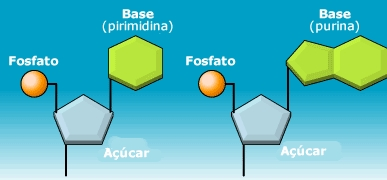
\includegraphics[angle=0,width=0.55\textwidth]{imagens//AcidosNucleicos.jpg}
\caption{Estrutura esquemática de um nucleotídeo, mostrando seus principais componentes: açúcar, fosfato e base nitrogenada~\citep{brainstuff:2000}. \label{fig:AcidosNucleicos}}
\end{figure}

A síntese dos ácidos nucléicos envolve ligações entre diferentes nucleotídeos, atráves dos grupos fosfato, por meio de uma ligação chamada ligação fosfodiéster. Nessa ligação, o átomo de fósforo estabelece fortes ligações covalentes com os átomos de carbono da pentose dos nucleotídeos.


\subsubsection{DNA} \label{sec:DNA}

O ácido desoxirribonucléico (DNA) contém as informações genéticas de um organismo vivo, com exceção de alguns vírus~\citep{silva:2001}. Nos organismos procariotos, o material genético está espalhado na célula. Nas células eucarióticas, o DNA está localizado no núcleo, e contém informações sobre como, quando e onde produzir cada tipo de proteína~\citep{lodish:2005}.


Uma molécula de DNA é formada por cadeias de nucleotídeos. As bases nitrogenadas, as quais constituem os nucleotídeos, podem ser divididas em dois grupos: purinas ou pirimidinas. Nas bases purinas encontram-se as bases formadas por dois anéis, a citosina (C) e a timina (T) e nas pirimidinas encontram-se as bases formas por anéis, a Adenina (A) e a Guanina (G).
Assim, existem quatro tipos de nucleotídeos, de acordo com sua base nitrogenada Figura~\ref{fig:nucleotideoDNA}, onde P representa o grupo fosfato, D a pentose (açúcar denominado de desoxirribose) as bases nitrogenadas que podem ser A, G, C ou T.

\begin{figure}[ht]
\centering
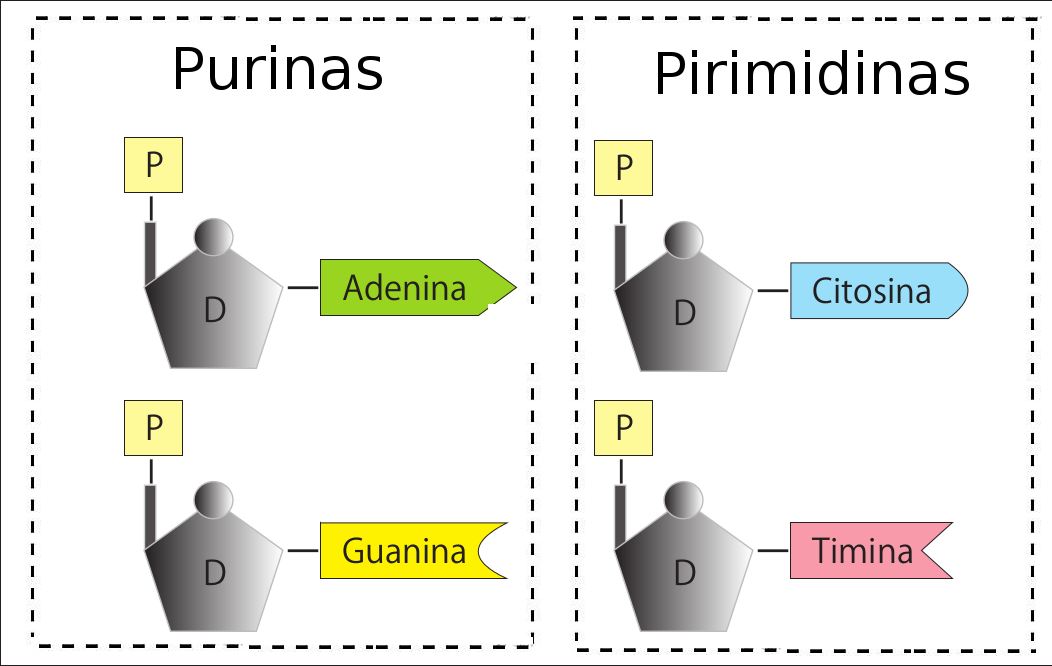
\includegraphics[angle=0,width=0.5\textwidth]{imagens//2007eu-nucleotideoDNA1}
\caption{Os quatros tipos de nucleotídeos que compõem a molécula de DNA.\label{fig:nucleotideoDNA}}
\end{figure}

A estrutura do DNA é formada por duas cadeias ou fitas paralelas compostas por uma sequência de nucleotídeos, que são unidas através de pontes de hidrogênio formadas entre as bases nitrogenadas de cada fita, onde a base A estará pareada com a base T (A-T) e C com G (C-G)~\citep{stryer:2002}. As bases A-T e C-G são chamadas de bases complementares. Essas duas fitas estão dispostas em espiral em torno de um eixo. Cada fita possui uma extremidade chamada 5' e a outra chamada 3', o que cria uma orientação em cada uma das fitas. As duas cadeias ficam, portanto em direção antiparalelas (opostas), formando uma dupla-hélice Figura~\ref{DNA-replicacao}.


O DNA pode sofrer replicações em alguns momentos através de um processo conhecido como duplicação semiconservativa, onde cada DNA recém formado possui uma das cadeias da molécula mãe~\citep{lopes:1998}.
Para realizar a replicação, a dupla fita do DNA abre-se, através do rompimento das pontes de hidrogênio, e os nucleotídeos livres encaixam-se na molécula através de novas pontes de hidrogênio. Os nucleotídeos vão sendo ligados entre si pela enzima DNA polimerase. O resultado desse processo é a formação de duas moléculas de DNA idênticas à original Figura~\ref{DNA-replicacao}.

\begin{figure}[ht]
\centering
\fbox{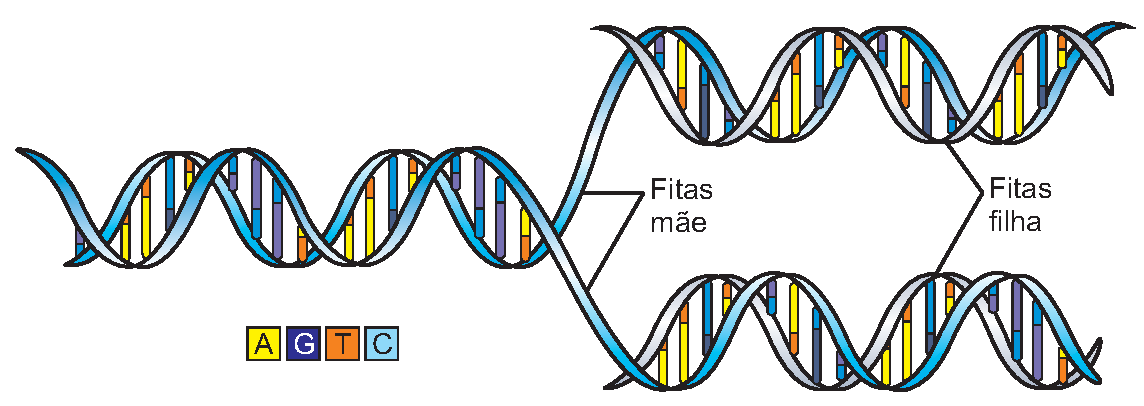
\includegraphics[angle=0,width=0.7\textwidth]{imagens//2005lodish-DNA-replicacao.pdf}}
\caption{Replicação DNA Semiconservativa. À esquerda podemos observar um trecho de uma molécula de DNA que evidencia o aspecto de dupla-hélice e à direita as fitas mãe separadas, servindo de molde para as filhas, resultando em duas moléculas idênticas à dupla-hélice original~\citep{lodish:2005}. \label{DNA-replicacao}}
\end{figure}

%\newpage
Algumas regiões do DNA possuem informações para codificar proteínas ou ncRNAs e são chamadas de genes. Esses genes são transcritos em RNAs, que realizam diversas funções, como catalíticas ou estruturais para síntese de proteínas ou regulação. Assim, a sequência de nucleotídeos do DNA é chamada de estrutura primária, ou seja, a estrutura primária é dada pela sequência linear formada ao longo da cadeia, sendo o nível estrutural mais simples~\citep{lodish:2005}. A estrutura secundária consiste no arranjo espacial da sequência.


\subsubsection{RNA} \label{sec:RNA}

De forma semelhante ao DNA, o ácido ribonucléico (RNA) é uma molécula constituída por cadeias de nucleotídeos, ou polinucleotídeo.


O RNA é também formado pelo grupo fosfato, açúcar (ribose) e por uma base nitrogenada. Porém, entre as bases nitrogenadas, a Uracila (U) substitui a Timina (T) do DNA~\citep{lodish:2005}. Assim, U é uma base purina. Na Figura~\ref{fig:nucleotideoRNA}, P representa o grupo fosfato, R a ribose e, em seguida, as bases nitrogenadas A, G, C e U.

\begin{figure}[ht]
\centering
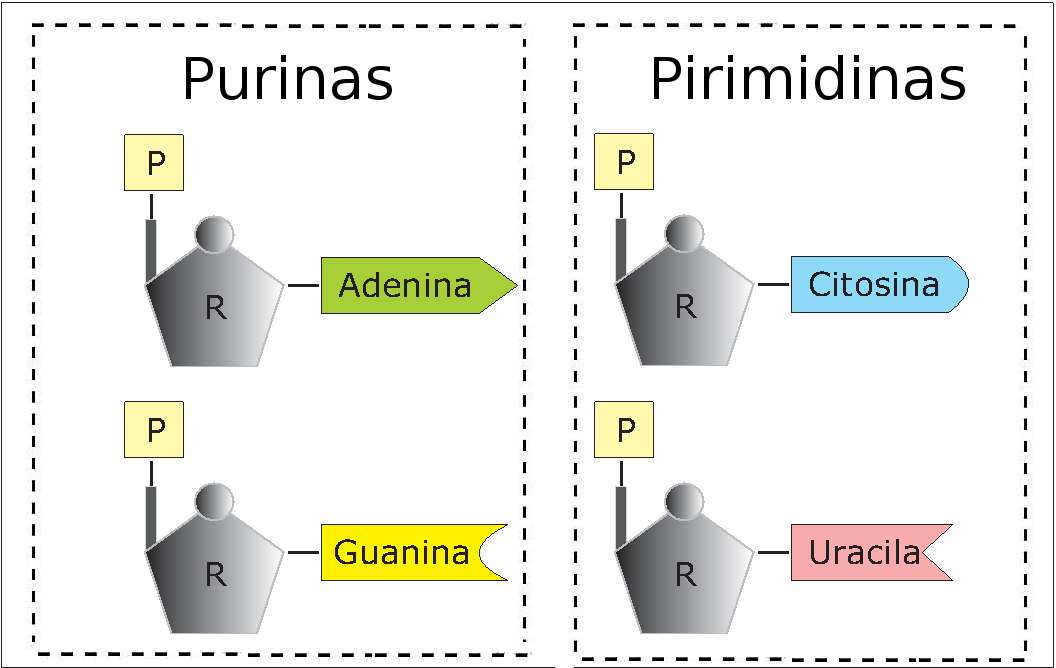
\includegraphics[angle=0,width=0.5\textwidth]{imagens//2007eu-nucleotideoRNA1}
\caption{Tipos de nucleotídeos que compõem a molécula de RNA, observando-se que a Uracila (U) substitui a Timina (T) nos RNAs. \label{fig:nucleotideoRNA}}
\end{figure}


O RNA é formado em geral por uma única fita de nucleotídeos, e não possui o aspecto de dupla-hélice~\citep{koolman:2005}. Porém, como o RNA tem como bases complementareas (A-U) e (C-G), pode unir-se através de pontes de hidrogênio, ou seja, o RNA pode dobrar-se.

Na síntese de proteínas estão envolvidos três tipos de RNAs, descritos com mais detalhes na Seção~\ref{sec:Dogma}: o mensageiro (mRNA), o ribossômico (rRNA) e o transportador (tRNA).


A Figura~\ref{fig:rRNA} mostra uma estrutura de um rRNA 16S da bactéria \textsl{Escherichia coli}. Esse RNA é o componente central dos ribossomos, que são organelas encontradas no citoplasma possuindo duas subunidades chamadas de 40S e 60S em células eucarióticas e 30S e 50S em bactérias~\citep{lafontaine:2001}. O mRNA é encontrado tanto no núcleo (onde ocorre sua síntese) quanto no citoplasma (onde participa da tradução de proteínas). Por último, vamos falar sobre os tRNAs, que são encontrados no citoplasma e funcionam durante a tradução, fazendo as ligações entre as proteínas e ácidos nucléicos. Esses RNAs são pequenos, contendo entre 70 e 90 nucleotídeos~\citep{koolman:2005}.

\begin{figure}[htb!]
\centering
\fbox{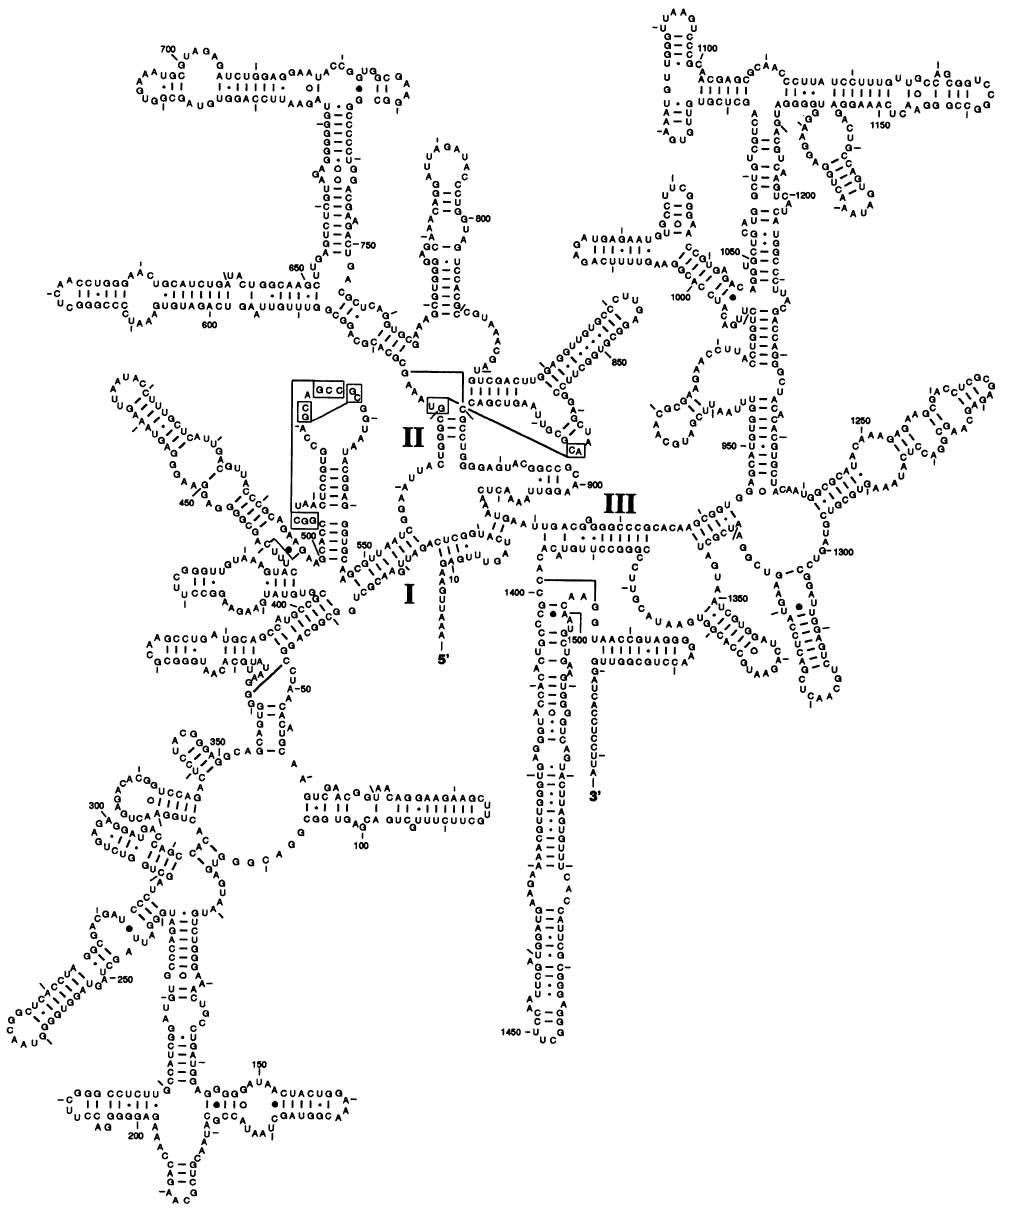
\includegraphics[angle=0,width=1.0\textwidth]{imagens//1994gutell-rRNA.jpg}}
\caption{Modelo da estrutura de um rRNA 16S da E.coli~\citep{gutell:1994}. \label{fig:rRNA}}
\end{figure}


\newpage
\subsection{Dogma Central da Biologia Molecular: Síntese de Proteínas}  \label{sec:Dogma}  % 2.4

Nesta seção, mostraremos como as informações presentes em uma molécula de DNA são utilizadas na síntese de proteína.


Em primeiro lugar, a transcrição ocorre no núcleo, e é sintetizada pela enzima RNA polimerase, que vai ligar-se a uma determinada sequência de nucleotídeos do DNA, identificadas pelas regiões promotoras, e a percorre utilizando-a como molde até encontrar as regiões terminadoras. A transcrição baseia-se no pareamento de bases complementares usando uma fita do DNA como molde, ou seja, adenina com uracila (A $\rightarrow$ U), timina com adenina (T $\rightarrow$  A) e citosina com guanina (C $\leftrightarrow$ G). A molécula de RNA recém sintetizada é o mRNA~\citep{lodish:2005}.

O processo de transcrição acontece tanto nos procariotos (não possuem núcleo celular) Figura~\ref{fig:processo-sintese-proteinaProc} como nos eucariotos (tem o DNA armazenado em um núcleo celular), tendo seu processo de transcrição um pouco mais complexo que os procariotos.

De acordo com~\citep{lodish:2005}, todos os organismos possuem maneiras de controlar quando os seus genes podem ser transcritos. Muitas células são capazes de responder a sinais externos ou a alterações nas condições externas, ligando ou desligando genes específicos, dessa forma, as células adaptam-se às necessidades do momento.

\begin{figure} [htb!]
\centering
\fbox{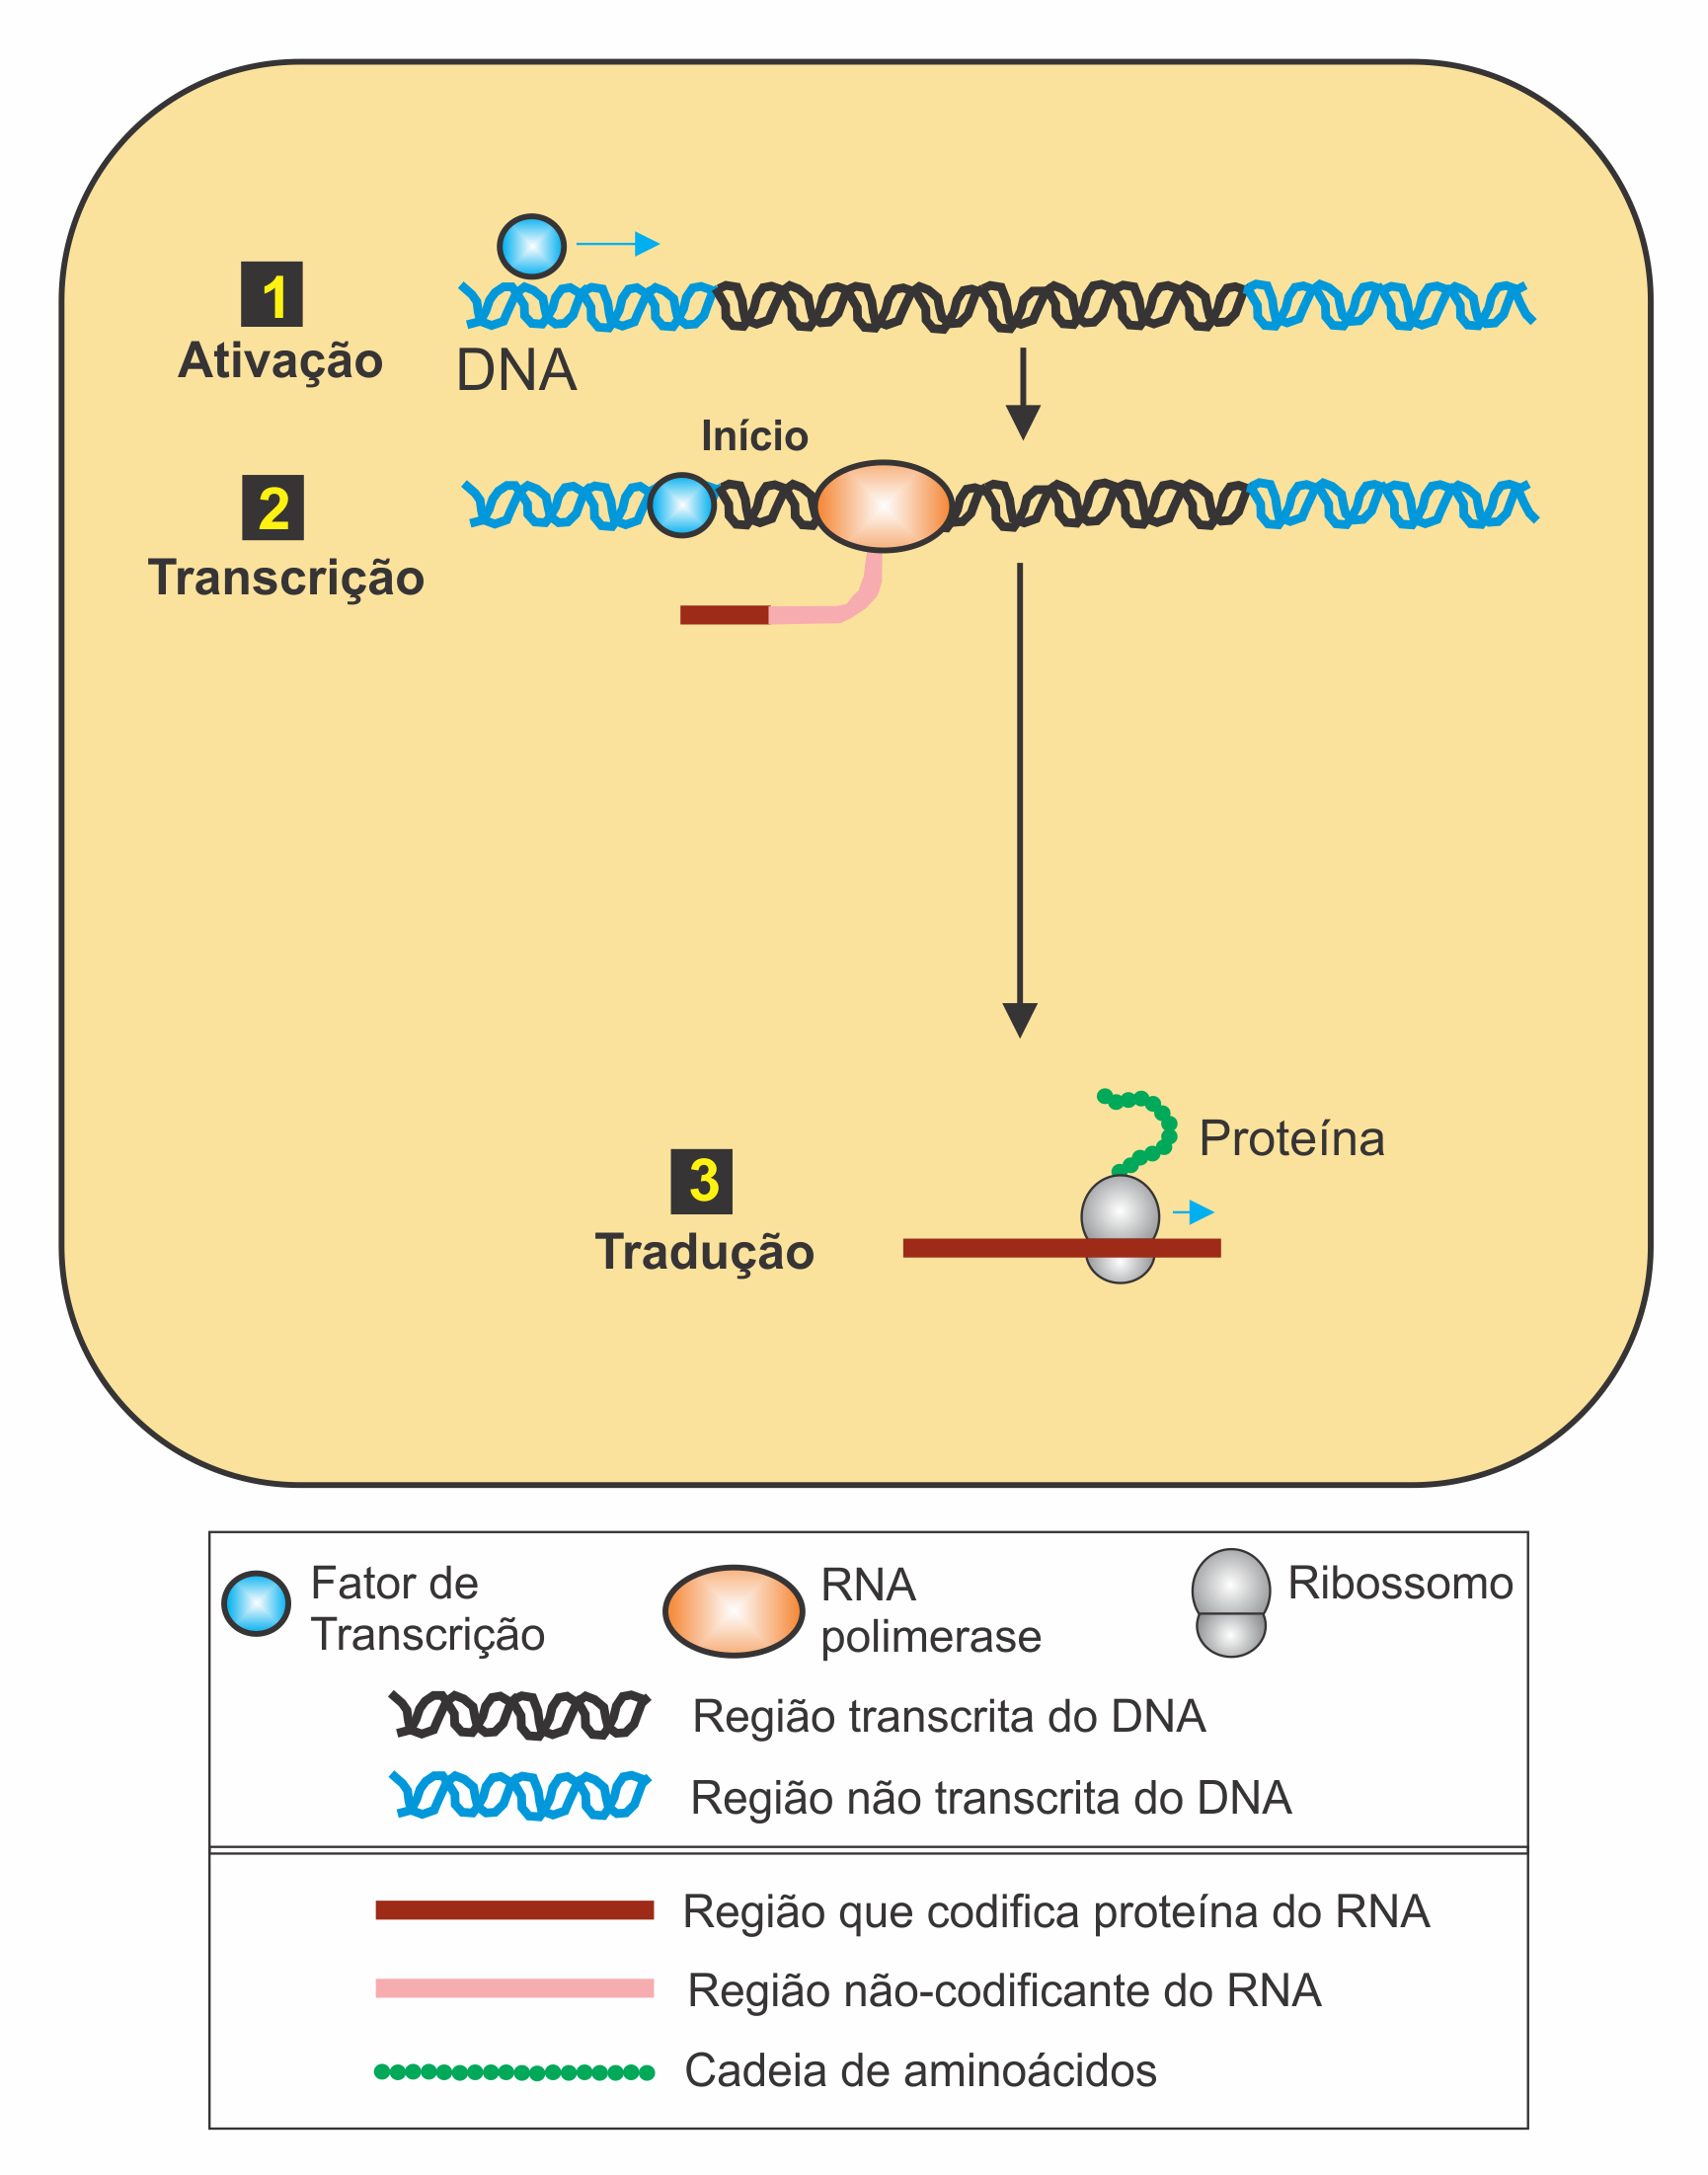
\includegraphics[angle=0,width=0.8\textwidth]{imagens//2005lodish-DNA-transcricao-traducaoProca.png}}
\caption{A síntese protéica em célula procariótica funciona da seguinte maneira. No passo 1, fatores de transcrição ligam-se às regiões da regulação dos genes que controlam, ativando-os. No passo 2, a RNA polimerase começa a transcrição do gene ativado pela região promotora, resultando na formação do mRNA. No passo 3, o mRNA e ligado no ribossomos. Nesse ponto, a proteína é sintetizada pelo ribossomo que liga os aminoácidos em uma cadeia linear ~\citep{lodish:2005}. \label{fig:processo-sintese-proteinaProc}}
\end{figure}

Nos eucariotos, o mRNA recém-trancrito é conhecido como pré-mRNA, e em alguns organismos ele irá sofrer algumas modificações antes que se transforme em um mRNA maduro~\citep{silva:2001}. No decorrer desse processo de maturação ocorre o \textsl{splicing} (eliminação dos íntrons do pré-mRNA) Figura~\ref{fig:processo-sintese-proteina}, que são regiões que não codificam a proteína~\citep{lodish:2005, Lundblad:2007}. 

\begin{figure} [htb!]
\centering
\fbox{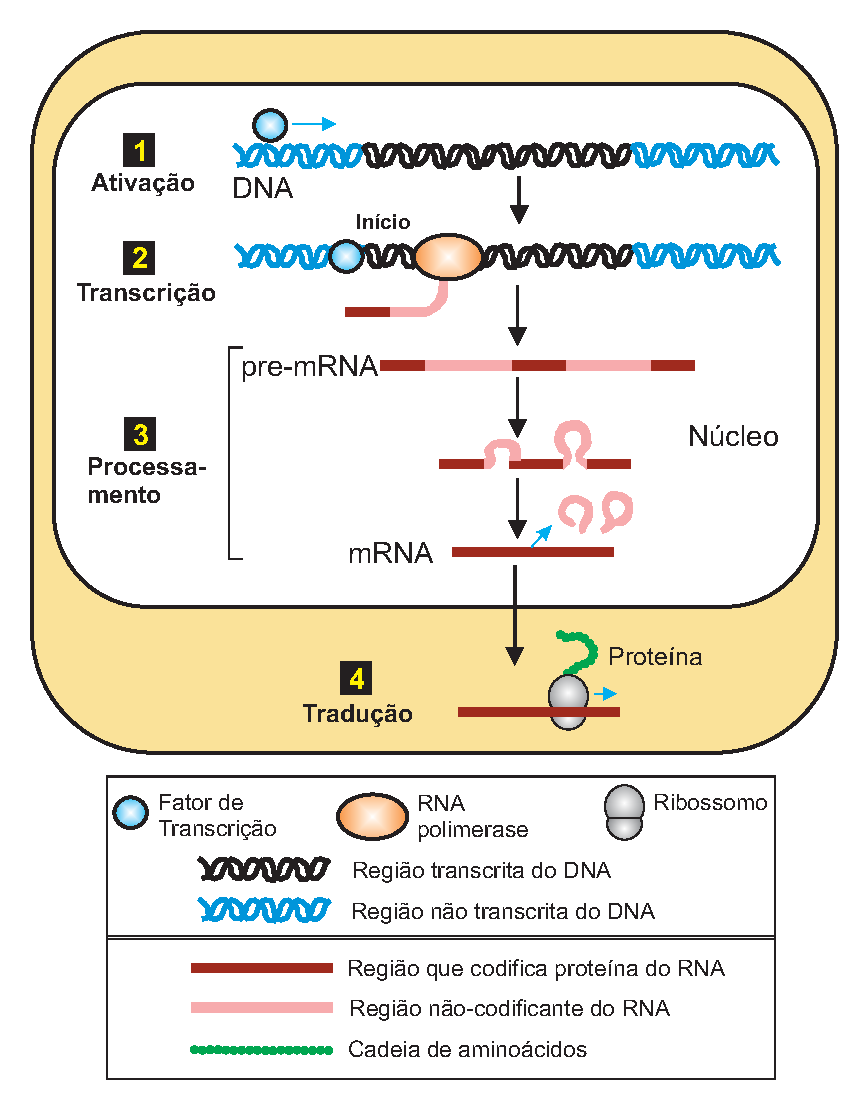
\includegraphics[angle=0,width=0.8\textwidth]{imagens//2005lodish-DNA-transcricao-traducao.pdf}}
\caption{A síntese protéica em célula eucariótica funciona da seguinte maneira. No passo 1, fatores de transcrição ligam-se às regiões da regulação dos genes que controlam, ativando-os. No passo 2, a RNA polimerase começa a transcrição do gene ativado pela região promotora, resultando na formação do pré-mRNA. No passo 3, é feito um processamento na transcrição para remover sequências não-codificadoras. Para finalizar, no passo 4, o mRNA move-se para o citoplasma e é ligado pelo ribossomos. Nesse ponto, a proteína é sintetizada pelo ribossomo que liga os aminoácidos em uma cadeia linear ~\citep{lodish:2005}. \label{fig:processo-sintese-proteina}}
\end{figure}

O mRNA formado através da transcrição move-se para o citoplasma, precisamente nos ribossomos, onde ocorre o segundo processo para a síntese da proteína: a tradução.

\newpage
No processo de tradução, primeiramente o mRNA liga-se entre as duas subunidades do ribossomo, onde cada códon do mRNA é pareado com o anticódon correspondente que está presente em moléculas de tRNA~\citep{silva:2001}. Cada aminoácido é codificado por um grupo de três bases do DNA, recebendo o nome de \textit{tríplex} ou \textit{códon}. Cada códon corresponde a um único aminoácido, porém um mesmo aminoácido pode ser definido por mais de um códon Tabela~\ref{fig:1995voet-aa}~\citep{silva:2001,lopes:1998}. Existem ainda três códons (UAG, UAA e UGA) que não correspondem a nenhum aminoácido, mas idicam sinais de término da tradução~\citep{silva:2001}. 

\begin{table}[ht]
\caption{O Código Genético~\citep{voet:1995}. \label{fig:1995voet-aa}}
\centering
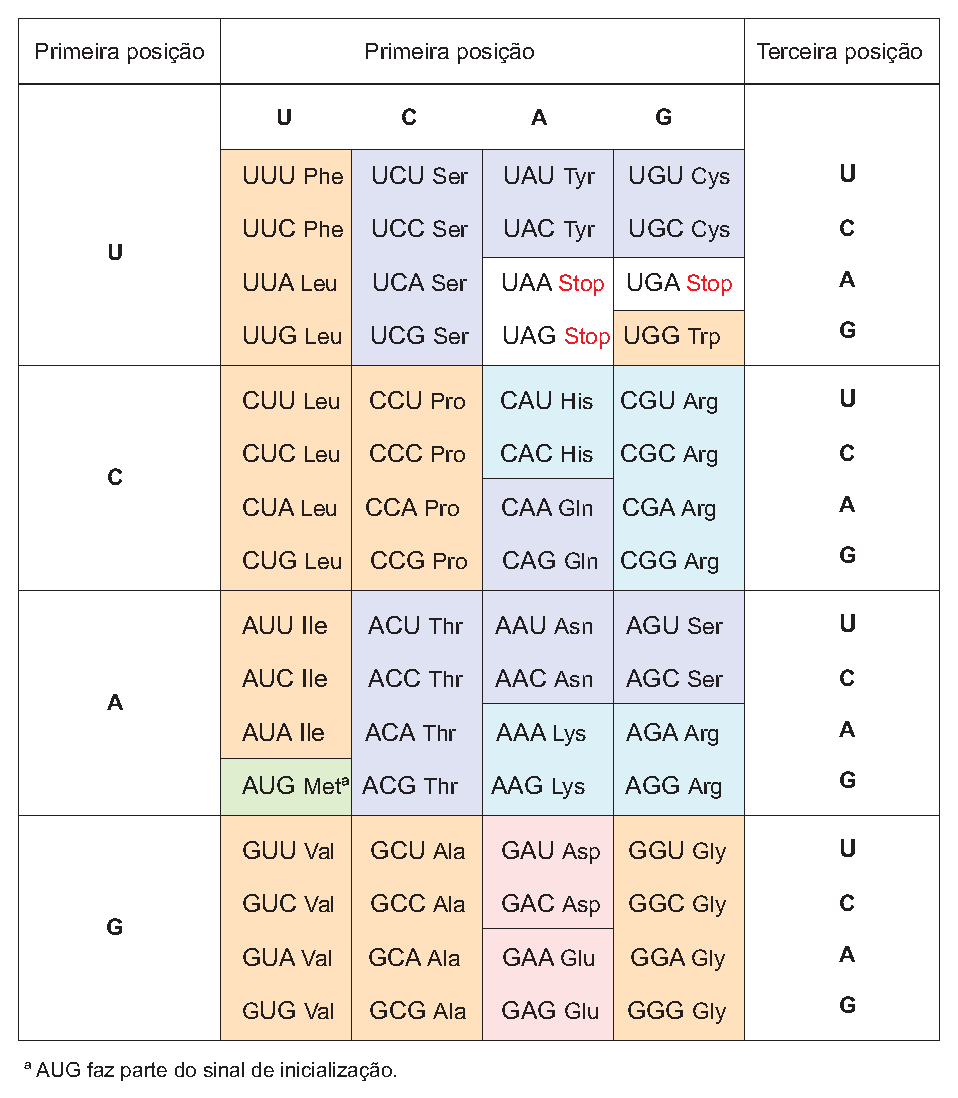
\includegraphics[angle=0,width=0.8\textwidth]{imagens//1995voet-aa}
\end{table}

Depois, é feito o pareamento do segundo tRNA, os aminoácidos são ligados e o primeiro tRNA é liberado. Esse processo é repetido até que apareça um sinal de terminação no mRNA, que vai resultar na formação de uma cadeia polipeptídica.

As proteínas são compostos orgânicos constituídos por aminoácidos unidos através de ligações peptídicas. Elas estão envolvidas em todos os processos biológicos dos seres vivos, como nas funções estruturais catalizadoras e reguladoras~\citep{liu:2006}.


\subsection{\textit{Pipelines} em projetos genoma} \label{sec:pipeline}

Em projetos de genomas, o sistema computacional é chamado \textit{pipeline}~\citep{Lemos:2004}, e é desenvolvido no laboratório de bioinformática. Descrevemos nesta seção, os \textit{pipelines} da antiga tecnologia Sanger e as modernas, chamadas de sequenciamento de nova geração.

    Já nas atuais tecnologias de processamento de alto desempenho, o \textit{pipeline} é dividido em outras fases, e fases semelhantes com objetivos diferentes.  A primeira fase o "mapeamento", busca alinhar os Expressed Sequence Tags (ESTs) obtidos durante um transcritoma com os de um genoma de referência, às vezes, o genoma do próprio organismo de onde os ESTs derivaram. No entanto, outros organismos podem ser utilizados. A fase de anotação apresenta certas diferenças tendo como principal objetivo  a identificação de RNAs não codificadores (ncRNA).


\subsubsection{Técnica: \textit{Sanger}}

Na antiga tecnologia de sequenciamento Sanger, o \textit{pipeline} é, em geral, dividido em três fases, \textbf{submissão}, \textbf{montagem} e \textbf{anotação}. A submissão visa receber as sequências geradas por sequenciadores automáticos a partir de experimentos realizados nos laboratórios de Biologia Molecular, transformando-as em cadeias de caracteres e armazenando-as em bancos de dados. Nota-se que estas sequências são fragmentos de DNA ou de RNA, pois a tecnologia sanger não consegue sequenciar o DNA inteiro nem mesmo mesmo uma molécula inteira de RNA.


\begin{figure} [htb!]
\centering
\fbox{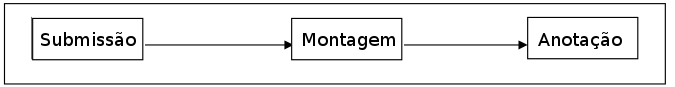
\includegraphics[angle=0,width=0.8\textwidth]{imagens//pipelineSange.png}}
\caption{\textit{pipeline} Sanger. \label{fig:pipeline-Sange}}
\end{figure}

Durante a fase de montagem, as sequências que provavelmente vieram da mesma região do DNA devem ser agrupadas. Cada grupo constituído de duas ou mais sequências é denominado de \textit{contig}, tendo cada \textit{contig} uma sequência resultante (consenso) do agrupamento de todas as sequências que o formam. As sequências que não puderam ser agrupadas são denominadas de \textit{singlets}. 

A última fase, denominada de anotação, consiste em associar funções biológicas às sequências resultantes da fase de montagem (consensos das \textit{contig} e \textit{singlets}), tomando funções conhecidas de sequências similares que estão disponibilizadas em bancos de dados biológicos públicos. Essa fase é dividida em duas etapas: automática e manual.

A anotação automática compara as sequências geradas no projeto com sequências de bancos de dados privados e/ou públicos~\citep{benson2006genbank:2006}. A comparação de duas sequências visa encontrar quais partes das sequências são parecidas ou similares. Dizemos que duas sequências são similares quando são "aproximadamente iguais", ou seja, têm exatamente os mesmos caracteres, com poucos caracteres diferentes, neste caso, podemos inferir que as duas sequências exercem o mesmo "papel biológico" ou têm a mesma função. Existem alguns métodos de comparação aproximada de sequências como BLAST~\citep{altschul1990basic:1990} e FASTA~\citep{pearson1988improved:1988}, bastante utilizados para inferir funções para as sequências identificadas em um projeto genoma.

Na anotação manual, são utilizadas as informações da anotação automática, bem como o conhecimento do biólogo, para determinar a função que vai ser associada efetivamente à sequência analisada.

Na \textbf{submissão} de um projeto genoma feito em sequenciadores Sanger, depois da recepção dos arquivos com os resultados do sequenciamento de cada fragmento (também denominado \textit{read}), um programa chamado \textit{Phred}~\citep{ewing1998base:1998}, traduzir as informações recebidas em sequências de letras contendo as bases identificadas e as probabilidades de erros associadas a cada base, gerando dois arquivos com extensão (\textit{.phd}), para cada \textit{read}. Depois, o programa \textit{Phd2Fasta} cria, pelo \textit{Phred}, dois arquivos texto no formato FASTA: um contendo a sequência de bases nitrogenadas e outro contendo os valores das probabilidades de erro.

A fase de submissao contém um grande numero de sequências, porém, nem todas são utilizadas nos próximos passos. Para ser utilizada, uma sequência deve possuir uma probabilidade de erro suficientemente baixa, sendo essa probabilidade determinada de acordo com cada projeto. Serão aceitas as sequências com qualidade mínima, o que aumenta a confiabilidade nos dados. 


O sequenciamento Sanger envolve cópias do DNA do organismo estudado, inseridas em um outro organismo. Assim, as sequências podem não pertencer ao organismo que está sendo estudado. Um programa chamado \textit{Cross match} visa identificar e retirar vetores e contaminantes das sequências. 
  

Na fase de \textbf{montagem}, são usado em geral dois programas, o \textit{CAP3}~\citep{huang1999cap3:1999} ou o \textit{Phrap}~\citep{green1994phrap:1994}. Estes programas geram arquivos FASTA contendo: as sequências de todos os \textit{singlets}; dados sobre a composição e sequências dos \textit{contigs}; e informações gerais sobre a montagem dos fragmentos de DNA.

Existe dois tipos de projetos de sequenciamento: genômico e transcritômico. No primeiro caso, para a identificação dos possíveis genes presentes nos \textit{contigs} e \textit{singlets} obtidos durante a montagem, utiliza-se o programa \textit{Glimmer}~\citep{salzberg1998microbial:1998}, para identificar ORFs. No caso de transcritomas, os \textit{contigs} e \textit{singlets} já codificam um gene, e assim, não há necessidade de se utilizar o \textit{Glimmer} para fazer a idenficação.


Por fim, na fase de \textbf{anotação} é utilizado o programa BLAST para fazer a comparação das sequências identificadas com bancos de dados de sequências cujas funções já são conhecidas na fase de anotação automática. Depois de feito esse procedimento, os bíologos podem proceder a anotação manual das sequências de acordo com seus conhecimentos.


Em todas etapas anteriormente descritas, são armazenadas estatísticas sobre o projeto, sendo algumas delas: o número de sequências aceitas e rejeitadas na fase de submissão, número de \textit{contigs} e \textit{singlets} encontrados (montagem), além de anotações manuais e automáticas.  


\subsubsection{Técnica: Alto-Desempenho} \label{sec:Sequenciamento}


No início da década de 2000, novas técnicas de sequenciamento massivamente pararelas revolucionaram a forma de realizar o sequenciamento do DNA. Com um custo muito baixo em comparação com o método Sanger, permitindo o sequenciamento de milhões de sequências, esses métodos tiveram um grande impacto nas áreas de pesquisa onde se realiza sequenciamento do DNA, e assim abriram novas frentes de pesquisas, como o estudo de DNAs antigos em mamutes, e diversidade ecológica por meio do sequenciamento de DNA de amostras ambientais~\citep{mardis2008next:2008}.

Nesta seção estudaremos o funcionamento de dois sequenciadores, o 454-FLX da Roche e o Illumina

\subsubsection*{454-FLX Roche} \label{sec:454}

O 454-FLX foi o primeiro sequenciador a aparecer no mercado, em 2004, utilizando uma técnica de sequenciamento conhecida com o nome de pirosequenciamento\citep{ronaghi1998sequencing:1998}. Essa técnica busca incorporar os nucleotídeo a uma fita de DNA por meio da enzima DNA polimerase que acarreta a liberação de pirofostato. Com isso a molécula inicia uma série de reações químicas cujo produto final é a liberação de luz. A detecção da luz e obtida por um sensor que permite a determinação das bases de uma sequência de DNA.


O 454-FLX Roche gera sequências de cerca de 250 a 600 bases de comprimento. Depois desse processamento, sequências com baixa qualidade são removidas, obtendo em cerca de milhões de bases com boa qualidade em média, com cerca de 1 milhão de \textit{reads}. O tamanho das sequências obtidas com o sequenciamento 454-FLX é menor que o sequenciamento Sanger, mas foi utilizado com sucesso no sequenciamento de genomas virais de bactériais com uma qualidade bastante alta.

Em geral, \textit{pipelines} para o 454 Roche envolvem uma fase de \textbf{filtragem}, que retira sequências com qualidades ruins, uma fase de \textbf{montagem}, feita por sobreposição de extremidades similares de sequências de entrada, e uma fase de \textbf{análise}, que inclui anotação.

\begin{figure} [htb!]
\centering
\fbox{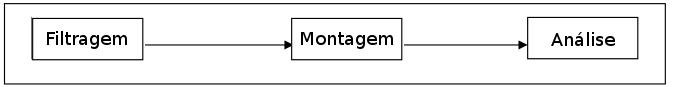
\includegraphics[angle=0,width=0.8\textwidth]{imagens//pipeline454.png}}
\caption{Um \textit{pipeline} genérico para o sequenciamento do 454 Roche. \label{fig:pipeline-454-FLX}}
\end{figure}


\subsubsection*{Illumina} \label{sec:Illumina}

A técnica de sequenciamento utilizada no Illumina incorpora um nucleotídeo por vez à sequência que está sendo determinada. Primeiro, realiza-se a amplificação de fragmentos do DNA, sendo incorporadoes adaptadores no início e fim de cada um dos fragmentos de DNA, que são anexandos a uma superfície. Depois disso, a DNA polimerase é utilizada para a produção de grupos de sequências, cada grupo contendo aproximadamente 1 milhão de cópias de fragmentos de DNA original.

Depois de amplificado o DNA, realiza-se o processo de sequenciamento em si. Nesse estágio, nucleotídeos fosforecentes são adicionados às moléculas de DNA amplificadas. Com a incorporação concluída, processa-se a imagem com as luzes oriundas dos nucleotídeos fosforecentes. Esse processo continua por um determinado número de ciclos, sendo controlado pelo operador do sequenciador, e podem ser construídas as sequências com 25 a 90 bases de comprimento, o que gera bilhões de bases sequenciadas, e cerca de 10 milhões de \textit{reads}~\citep{dohm2008substantial:2008}.

Um \textit{pipeline} para Illumina inclui uma fase de \textbf{mapeamento}, onde as \textit{reads} de tamanho curto são mapeadas em um genoma de referência, e uma fase de \textbf{análise}, que inclui estatísticas de cobertura de \textbf{análise} de expressão diferencial, por exemplo. 

\begin{figure} [htb!]
\centering
\fbox{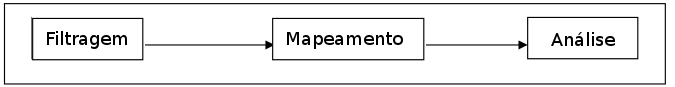
\includegraphics[angle=0,width=0.8\textwidth]{imagens//pipelineIllumina.png}}
\caption{Um \textit{pipeline} genérico para o sequenciamento do Illumina. \label{fig:pipeline-Illumina}}
\end{figure}

 % cap 2

  \chapter{RNAs não-codificadores}
\label{sec:ncRNACodificadores}

Neste capítulo descreveremos os RNAs não-codificadores (ncRNAs), que serão objeto de estudo deste trabalho de doutorado. Na seção~\ref{sec:ConBasico}, estudamos ncRNAs de forma geral. Na Seção \ref{sec:ClassNCrnas}, são apresentadas classificações e descrições dos ncRNAs. Em seguida, na Seção~\ref{sec:FerraCompDet}, são descritas algumas ferramentas computacionais para detecção de ncRNAs das classes conhecidas. Na Seção~\ref{sec:bd-ncRNA}, mostraremos os bancos de dados utilizados. Na Seção~\ref{sec:CaracDesafDetec}, seguem características e desafios na detecção de ncRNAs, que serviram de motivaram para esta pesquisa.


\subsection{Conceitos Básicos} \label{sec:ConBasico}

RNA não-codificadores (ncRNA) são tipos específicos de RNA que não codificam proteínas~\citep{watson1953molecular:1953,eddy2001non:2001}, entretanto sua conformação permite que desempenhem funções em vários processos celulares.

O primeiro enunciado do Dogma Central da Biologia Molecular dizia que a função dos RNAs, restringia-se a participação em síntese de proteínas. Contudo, estudos recentes revelam que a quantidade de ncRNAs equivale a 98\% do genoma humano. Uma quantidade tão grande de ncRNAs não pode simplesmente estar sendo produzida sem razão. Portanto atualmente vários estudos  pretendem compreender melhor o papel desses RNAs nos organismos.

	
Apesar de identificados, e possuírem papel de grande importância, a caracterização dos RNAs não-codificadores foi, nas décadas de 1980 e 1990, abandonada e relegada para um segundo plano, talvez devido a dificuldades técnicas relacionadas a identificar essas moléculas pequenas, instáveis e pouco abundantes~\citep{eddy2001non:2001}. Nesta época, os RNAs não envolvidos diretamente com a síntese de proteínas eram chamados de DNA lixo (\textit{junk} DNA)
~\citep{setubal1997introduction:1997}.


	A partir do início dos anos 2000, retomaram-se os estudos dos ncRNAs, em consequência da crescente quantidade de ncRNAs identificados pelos biólogos e descritos na literatura. As descobertas mais notáveis envolvendo RNAs estruturais estão relacionadas ao desenvolvimento do sistema nervoso, corroborando a observação de que a quantidade de regiões não-codificadoras é proporcional à complexidade dos organismos ~\citep{badger1999critica:1999,mattick2001evolution:2001,mercer2008specific:2008,presutti2006non:2006}. Além dos \textit{small interfering} RNA (siRNA) e micro RNAs (miRNA) que ocorrem nos organismos, foram desenvolvidos novos métodos artificiais baseados nos mecanismos nos quais esses RNAs estavam envolvidos, citando principalmente silenciamento de RNAs mensageiros alvo, que já são empregados com sucesso~\citep{reynolds2004rational:2004}.


	Os métodos computacionais para identificar ncRNAs sofrem de problemas similares aos dos métodos experimentais. A Bioinformática não possui métodos únicos para identificação e classificação de ncRNAs, embora alguns critérios sejam usados, como: o fato de que ncRNAs não possuem em geral ORFs longas; há ao longo de sua sequência ocorrências de códons de parada maiores do que a esperada~\citep{wahlestedt2006natural:2006}; provavelmente RNAs tem uma conservação em nível de estrutura secundária e não primária, o que invalida a detecção de ncRNAs por meio de ferramentas tradicionais usadas para caracterizar similaridade de DNA em proteínas \citep{pang2006rapid:2006,rivas2001noncoding:2001,torarinsson2006thousands:2006}. Estudos que incorporam uso de códons, substituições sinônimas e não-sinônimas e energia mínima de dobramento também são bem-sucedidos na identificação de ncRNAs~\citep{badger1999critica:1999,torarinsson2006thousands:2006,xue2005classification:2005}.
	
	Geralmente, os ncRNAs não possuem uma sequência conservada, tendo como principal característica a conservação de sua estrutura espacial que inclui bidimensional ou tridimensional, tornando sua identificação mais difícil. Os ncRNAs mais conhecidos  possuem uma estrutura tridimensional complexa e têm funções tanto catalisadoras como estruturais ~\citep{eddy:2002}. A atual tendência dos métodos de Bioinformática é recorrer a uma combinação de diversos métodos computacionais que caracterizem os ncRNAs por meio de diferentes princípios, e depois analisar todas as informações geradas pelos métodos para decidir quais RNAs provavelmente são
não-codificadores~\citep{mignone2006discrimination:2006,liu:2006}.
	
	
	Sabendo que o problema na busca de ncRNA é essencialmente de classificação,  a escolha de um método depende dos dados disponíveis das sequências que estão sendo analisadas~\citep{rivas2001noncoding:2001,wang2006psol:2006}.  Uma desvantagem é que para confirmar a predição feita \textit{in silico} de um transcrito computacional ser codificador, que exige validação experimental no laboratório, a observação de ausência de tradução não é conclusiva, já que o eventual transcrito poderia ser traduzido logo que exposto a outras condições, ambientais ou fisiológicas~\citep{mignone2006discrimination:2006,liu:2006}.


Desde a descoberta dos ncRNAs, muitas perguntas têm sido feitas e muitos estudos têm sido direcionados à procura de respostas. Porém, essas moléculas ainda não são bem conhecidas. A principal causa disso é que maior parte das pesquisas para detecção de genes, durante muito tempo, foram voltadas na direção de RNAs mensageiros e proteínas.


\subsection{Classificações de ncRNAs} \label{sec:ClassNCrnas}

Os ncRNAs, são classificados, em geral, de acordo com suas funcionalidades, o que permite entender diferentes aspectos relacionados às suas sequências genômicas e, portanto, ao papel que os ncRNAs realizam nos mecanismos celulares. Na Tabela~\ref{fig:ClassncRNAs} são tratadas classes de ncRNAs importantes.

\begin{table}[ht]
 \scalefont{0.8}
 \caption{Alguns tipos de ncRNAs e suas funções conhecidas~\citep{setubal1997introduction:1997,eddy2001non:2001}} \label{fig:ClassncRNAs}\begin{tabular}{|c|l|l|}
\hline
\multicolumn{ 3}{|c|}{\textbf{Classes de ncRNAs}} \\ \hline
\textbf{Sigla} &  \textbf{Função}   & \textbf{Referências} \\ \hline
tRNA &  envolvidos na tradução de mRNAs &~\citep{pavon2009trna:2009}\\ \hline
rRNA &  RNA constituinte do ribossomo &~\citep{eddy2001non:2001} \\ \hline
snoRNA &  envolvidos na modificação do rRNA &~\citep{durbin1998biological:1998}  \\ \hline
miRNA &  família putativa de genes reguladores da tradução. &~\citep{mendell2005micrornas:2005}  \\ \hline
siRNA &  moléculas ativas na interferência de RNA &~\citep{eddy2001non:2001}\\ \hline
piRNA &  regulação de tradução e estabilidade de mRNA, entre outras &~\citep{brennecke2007discrete:2007}  \\ \hline
snRNA &  incluem RNAs relacionados ao processo de excisão &~\citep{stryer:2002}\\ \hline
snmRNA &  essencialmente pequenos RNAs não-codificadores &~\citep{huttenhofer2001rnomics:2001}  \\ \hline
stRNA &  interrompem a tradução de mRNA &~\citep{eddy2001non:2001}  \\ \hline
rasiRNA &  silenciamento da transcrição via remodelagem da cromatina &~\citep{xie2004genetic:2004}  \\ \hline
\end{tabular}
\label{}
\end{table}


O \textbf{RNA transportador (tRNA)}~\citep{pavon2009trna:2009} é utilizado como molécula transportadora de informação de cada códon componente do mRNA em um aminoácido específico a ser adicionado à proteína sendo formada. O tRNA desempenha essa função através de duas regiões, o anticódon que é responsável pelo reconhecimento de códons específicos do mRNA, e o aminoácido correspondente ao códon.

O \textbf{RNA ribossomal (rRNA)}~\citep{eddy2001non:2001} é o componente central do ribossomo. A função do rRNA é prover um mecanismo para decodificar o mRNA em aminoácidos e interagir com os tRNAs durante a tradução, de síntese de proteína.

O \textbf{\textit{small nucleolar} RNA (snoRNA)}~\citep{durbin1998biological:1998} é uma classe de pequenas moléculas que realizam modificações químicas no rRNA, além de outros ncRNAs, tal como o tRNA. Essas modificações possuem como principal objetivo promover a maturação desses ncRNAs, transformando-os em moléculas ativas. A origem desses genes ainda não está clara, mas acredita-se que eles originam-se dos íntrons do mRNA.

O \textbf{microRNA (miRNA)}~\citep{mendell2005micrornas:2005} parece estar relacionado com a regulação gênica. As moléculas de miRNA são parcialmente complementares a uma ou mais moléculas de mRNA e sua principal função é reduzir a expressão de genes codificadores, inibindo a tradução de mRNAs.

\textbf{\textit{small interfering} RNA(siRNA)}~\citep{eddy2001non:2001} possui o mesmo papel do miRNA, porém reduz a expressão de genes codificadores degradando o mRNA em vez de inibir sua tradução.

\textbf{\textit{piwi-interacting} RNA (piRNA)}~\citep{brennecke2007discrete:2007} é uma classe de pequenas moléculas de RNA existentes basicamente nas células de mamíferos. Assim como os miRNAs e os snoRNAs, os piRNAs também estão relacionados com a regulação gênica. Mais especificamente, eles atuam no silenciamento de genes capazes de se auto-duplicar no interior do genoma.

%\textbf{\textit{functional} RNA (fRNA)}~\citep{carter2001computational:2001} é uma molécula que provê a relação entre a tripla do código genético e os aminoácidos codificados


\textbf{\textit{Small nuclear} RNA (snRNA)}~\citep{stryer:2002} é uma classe de RNAs não-codificantes encontrados no interior do núcleo das células. O núcleo contém muitos tipos de snRNAs. A estrutura secundária desses RNAs é altamente conservada nos organismos. Alguns deles, conhecidos como U1, U2, U4, U5 e U6, são essenciais para o \textit{splicing} do pre-mRNA.


\textbf{\textit{small non-messenger} RNA (snmRNA)}~\citep{huttenhofer2001rnomics:2001} é uma classe de ncRNAs, com função reguladora.


\textbf{\textit{Small temporal} RNA (stRNA)}~\citep{eddy2001non:2001} é uma classe de RNAs com função de regulação do desenvolvimento biológico.

\textbf{\textit{repeat-associated} siRNA (rasiRNAs)}~\citep{xie2004genetic:2004} estão envolvidos na manutenção da metilação do DNA e histonas em retrotranposons, são sequências repetitivas como as codificadoras de RNA
ribossomal. A formação de heterocromatina, que ao nível do DNA é composta de sequências de retrotransposons degenerados e arranjos em tandem de unidades de repetições simples, também é mediada por rasiRNAs.


\subsection{Ferramentas computacionais para detecção de ncRNAs} \label{sec:FerraCompDet}

Nesta seção, descrevemos ferramentas para identificar e classificar de ncRNAs.


\subsubsection*{BLAST}

O programa \textit{Basic Local Alignment Search Tool} (BLAST)~\citep{altschul1990basic:1990} é bastante utilizado na comparação entre sequências. É um método de alinhamento local, que compara uma sequência com outras sequências com funções já definidas em um banco de dados. O BLAST pode ser utilizado para identificar relação evolucionária, inferir funções ou identificar uma família de genes entre sequências.

O BLAST é constituído por uma série de programas:

\begin{itemize}
\item \textbf{blastp}: para comparação de sequências de aminoácidos com um banco de dados
de proteínas;
\item \textbf{blastn}: para comparação de sequências de nucleotídeos com banco de dados
de DNA;
\item \textbf{blastx}: para comparação de sequências de nucleotídeos traduzida em
todas as ORFs com banco de dados de proteínas;
\item \textbf{tblastn}: para comparação de sequências de proteínas com um banco de dados
de sequências de nucleotídeos traduzidas em todas as suas ORFs;
\item \textbf{tblastx}: para comparar as ORFs de sequências de nucleotídeos com todas as
ORFs de um banco de dados de nucleotídeos.
\end{itemize}

%Para efetuar uma breve análise da estrutura do BLAST, obteve-se o pacote com os códigos-fontes das ferramentas do NCBI - \textit{ncbi-tools}. Esse pacote está disponível no servidor FTP\footnote{BLAST FTP - Disponível em [ftp://ftp.ncbi.nih.gov/ ]} do NCBI. O pacote está disponível no arquivo ncbi.tar.gz.

\subsubsection*{Infernal}

O Infernal (\textit{INFERence of RNA Alignment}) é um método que utiliza uma abordagem baseada em Gramática Estocástica Livres de Contextos (SCFG, \textit{Stochastic Context-Free Grammars})~\citep{eddy1994rna:1994,sakakibara1994stochastic:1994}. Essa ferramenta constrói perfis de RNA consenso chamados de modelos de covariância (CM, \textit{Covariance Models}), que é um caso especial de SCFG projetado para modelar sequências e estruturas de RNAs. O Infernal usa esses CMs para procurar as semelhanças entre as estruturas secundárias das famílias de RNAs do banco de dados Rfam e da sequência com qual está sendo investigada.


 Cada CM é construído a partir do alinhamento múltiplo de sequências e de dados relacionados à estrutura secundária consenso, em posições onde o alinhamento é único e onde ocorrem pareamento de bases. Pontuações são atribuídas para cada posição específica assim como para quantidades de nucleotídeos, pareamento de bases, inserções e deleções.


 O Infernal compreende os programas \textit{cmbuild} , \textit{cmsearch} e \textit{cmalign}. A construção do CM, feita pelo \textit{cmbuild}, requer como entrada um alinhamento múltiplo de RNAs no formato Estocolmo (\textit{Stockholm})~\citep{eddy2003infernal:2003}, gerando um arquivo de saída contendo o modelo de covariância, o qual será usado por outras funções do Infernal. 
 
 A busca em bases de dados por possíveis homólogos, feitas pelo \textit{cmsearch} requer duas entradas: um arquivo CM (obtido com o \textit{cmbuild}); e um arquivo contendo as sequências a serem analisadas.

O \textit{cmsearch} busca as sequências que geraram \textit{hits} com alta pontuação para o modelo de convariância usado. É gerada uma saída contendo os alinhamentos para cada \textit{hit} em um formato similar a estrutura BLAST~\citep{altschul1990basic:1990}. Já o alinhamento de possíveis homólogos, utilizando o \textit{cmalign} requer um arquivo de CM e outro arquivo que contenha possíveis homólogos. Este programa alinha sequências de acordo com o CM, criando um alinhamento múltiplo no formato Estocolmo. Esse alinhamento poderá ser utilizado como entrada na construção de um modelo de covariância pelo \textit{cmbuild}, como descrito acima.


Dentro da ferramenta Infernal, existe um módulo chamado \textit{Rsearch}, que compara
sequências de RNAs com um banco de sequências conhecidas de RNAs. Desta
forma, dada uma sequência de RNA, são feitas buscas em uma base de dados de
nucleotídios por RNAs homólogos. Esta busca é baseada tanto na estrutura primária quanto na estrutura secundária~\citep{klein2003rsearch:2003}.

Os algoritmos de alinhamento desta ferramenta são baseados em gramáticas estocásticas livres de contexto (SCFG, \textit{Stochastic Context-Free Grammars})~\citep{eddy1994rna:1994,sakakibara1994stochastic:1994}. Incorporada aos algoritmos de alinhamento, existe uma matriz de substituição apropriada para RNAs denominada RIBLOSUM~\citep{klein2003rsearch:2003}, similar às matrizes usadas para proteínas, como a BLOSUM~\citep{henikoff1992amino:1992}.


\subsubsection*{tRNAscan-SE}

O programa tRNAscan-SE~\citep{lowe1997trnascan:1997} é considerado um dos preditores de tRNAs mais precisos~\citep{laslett2004aragorn:2004}. Ele combina três programas: dois preditores de tRNAs que buscam promotores de RNA polimerase III e características da estrutura secundária~\citep{fichant1991identifying:1991,pavesi1994identification:1994}, além de usar um Modelo de Covariância~\citep{eddy1994rna:1994} treinado com sequências de tRNAs. Os dois primeiros programas são rápidos e, quando combinados, possuem uma sensibilidade superior a aproximadamente 99\%. Porém, tal combinação implica em uma taxa de aproximadamente 1.85 falsos positivos por MB, o que é aceitável para genomas pequenos, mas significa aproximadamente 5.500 falsos positivos no genoma humano.

O Modelo de Covariância é bastante sensível e específico, mas muito lento. Portanto, os dois primeiros preditores de tRNAs são utilizados com baixa estringência como filtros a fim de obter candidatos promissores de tRNAs de um genoma. Os candidatos são então analisados pelo modelo de covariância, altamente estringente. O resultado é um identificador de tRNAs apresentando alta sensibilidade (99-100\%) e seletividade (com uma taxa de falsos positivos inferior a 0.00007 por Mb) com uma velocidade razoável (30 Kb/s).


\subsubsection*{SVM-Portrait}

O SVM-Portrait~\citep{Arrial:2006,arrial2009screening:2009} é adequado para identificar ncRNAs de transcritomas incompletos ou de espécies cujas caracterizações não foram concluídas. Essa ferramenta utiliza-se de métodos baseados em técnica de aprendizagem de máquina, particularmente Máquina de Vetor de Suporte (\textit{Support Vector Machine} - SVM). O resultado do SVM-Portrait é a probabilidade de uma sequência não codificar uma proteína.



\subsubsection*{Vienna}

O Vienna~\citep{hofacker1994fast:1994} é um pacote utilizado em pesquisas que geram ou comparam estruturas secundárias de RNAs. Esse pacote tem várias ferramentas, em que dobramentos são feitos utilizando um algoritmo de predição basendo na energia livre do RNA~\citep{zuker1984rna:1984}, e nas probabilidades de pareamento de bases~\citep{mccaskill1990equilibrium:1990}. 

Dentro do Vienna, o pacote RNAz, realiza a predição de estrutura baseada na energia mínima livre (MFE, \textit{Minimun Free Energy})~\citep{zuker1981optimal:1981,hofacker1994fast:1994}. É levado em consideração o fato de que as estruturas dos ncRNAs apresentam duas características: a estabilidade termodinâmica e a conservação da estrutura secundária~\citep{gruber2007rnaz:2007}. Para o primeiro critério, o RNAz calcula uma medida normalizada da estabilidade termodinâmica e a seguir uma pontuação (z-\textit{score}) é gerada. Uma pontuação mais negativa indica que a sequência é mais estável do que a esperada ao acaso~\citep{gruber2007rnaz:2007}.

Para o segundo critério, o RNAz prediz uma estrutura secundária consenso de um alinhamento usando a abordagem RNAalifold~\citep{hofacker2002secondary:2002}. Mutações compensatórias (mutações que preservam um par de bases correto, por exemplo, substituição do par CG pelo par UA) são pontuadas, enquanto que mutações inconsistentes (a substituição do par CG por CA, por exemplo adicionam penalidades). No final, é calculado o índice de conservação da estrutura (SCI, \textit{structure conservation index})~\citep{gruber2007rnaz:2007}.

Finalmente, o RNAz utiliza um algoritmo de aprendizado de máquina SVM, que foi treinado utilizando um vasto conjunto de ncRNAs conhecidos. Esta etapa utiliza os resultados do critério (z-\textit{score}) para classificar o alinhamento de entrada como "RNA estrutural" ou "outros"~\citep{gruber2007rnaz:2007}.


Dentro do Vienna, o pacote RNAfold~\citep{hofacker2003vienna:2003} explora a hipótese de que uma molécula de RNA é dobrada na estrutura termodinamica mais estável, isto é, aquela que tem a energia livre mínima (ELM). Uma abordagem direta seria enumerar todas as possíveis estruturas e então selecionar aquela com o valor mínimo de energia livre~\citep{pipas1975method:1975}.   


\subsubsection*{RNAmmer}

O RNAmmer~\citep{lagesen2007rnammer:2007} é uma ferramenta de predição de rRNAs que utiliza os bancos de dados 5S \textit{ribosomal database} e \textit{European ribosomal RNA database} para gerar os diversos alinhamentos estruturais necessários para à construção de bibliotecas de cadeias de Markov. 


\begin{table}[ht]
\scalefont{0.8}
 \caption{Ferramentas computacionais} \label{fig:FerrRNAs}\begin{tabular}{|c|l|l|}
\hline
%\multicolumn{ 3}{|c|}{\textbf{Ferramentas}} \\ \hline
\textbf{Nome} &  \textbf{Descrição}   & \textbf{Referências} \\ \hline
BLAST & Compara informações de sequências biológicas primária &~\citep{altschul1990basic:1990}\\ \hline
Infernal & Baseado em Gramática Estocástuca Livres de Contextos &~\citep{eddy1994rna:1994} \\ \hline
tRNAscan-SE & Usa modelo de covariância na predição de tRNAs&~\citep{lowe1997trnascan:1997}  \\ \hline
SVM-Portrait & Identifica ncRNAs de transcritomas incompletos &~\citep{Arrial:2006}  \\ \hline
Vienna &  Compara estruturas secundárias de RNAs &~\citep{hofacker1994fast:1994}\\ \hline
RNAmmer & Usa cadeia de Markov na predição de rRNAs&~\citep{lagesen2007rnammer:2007}\\ \hline
\end{tabular}
\label{}
\end{table} 


\subsection{Bancos de dados} \label{sec:bd-ncRNA}

Nesta seção descrevemos os bancos de dados usados para detecção de ncRNAs. Esse respositóriso são criados tanto a partir de dados experimentais quanto computacionais~\citep{solda2009ariadne:2009}.

\subsubsection*{NONCODE}

Todos os ncRNAs do NONCODE~\citep{NONCODE:2012} foram filtrados automaticamente da literatura e do GenBank~\citep{Genbank:2012} e, em seguida, tratados manualmente. O NONCODE inclui quase todos os tipos de ncRNAs, exceto tRNAs e rRNAs. Mais de 80\% das entradas do NONCODE estão baseadas em dados experimentais. A primeira versão do NONCODE (v1.0) continha 5.339 sequências de 861 organismos, hoje na versão v3.0 com mais de 411.552 ~\citep{liu2005noncode:2005}.

\subsubsection*{RNAdb}
O RNAdb~\citep{RNAdb:2012} é um banco de dados de ncRNAs de mamíferos que contém sequências e anotações de milhares de ncRNAs, mas a maioria com papéis ainda não esclarecidos~\citep{pang2007rnadb:2007}.

\subsubsection*{miRBase}
miRBase~\citep{miRBase:2012} é um banco de dados de microRNAs ~\citep{jones:2006}.

\subsubsection*{snoRNA Database}
A base de dados snoRNAbase~\citep{snoRNAbase:2012,lestrade2006snorna:2006} contém snoRNAs humanos do tipo H/ACA e C/D \textsl{box}.


\subsubsection*{snoRNAs de plantas}
O \textsl{Plant snoRNA Database} contém snoRNAs de plantas~\citep{PlantsnoRNA:2012,brown2003plant:2003}.

\subsubsection*{fRNAdb}
O fRNAdb~\citep{mituyama2009functional:2009} integra um conjunto de outras base de dados, dentre outros o NONCODE
e o RNAdb.

%\subsubsection*{NRED}

%\subsubsection*{NATsDB}

%\subsubsection*{Trans-SAMap}

%\subsubsection*{antiCODE}

%\subsubsection*{smiRNAdb}

%\subsubsection*{microrna.org}

%\subsubsection*{Argonaute}

%\subsubsection*{Tarbase}

%\subsubsection*{MirGator}
%O MirGator é um banco de dados utilizado para interpretar funcionalidades de miRNAs.

\subsubsection*{Rfam}

O Rfam é uma base de dados curada (revisada e supervisionada), contendo informações sobre as famílias de ncRNAs. Esta base de dados consta de duas classes distintas de dados: os perfis de modelos de covariância (CMs) e os alinhamentos semente (\textit{seed alignments}). Como dito anteriormente, os CMs são modelos estatísticos resultantes da combinação de informações tais como estrutura secundária e sequências primárias, representadas pelo alinhamento múltiplo de sequências. Cada perfil de CM corresponde a uma família de ncRNA. Já os alinhamentos semente  estão contidos dentro de um arquivo no formato Estocolmo e contém os membros representativos de cada família de ncRNA gerados através de diversos alinhamentos estruturais~\citep{griffiths2003rfam:2003}.


Os arquivos Rfam podem ser obtidos do site de FTP do Sanger~\citep{Rfam:2012}. Nesse trabalho foi utilizado o Rfam 10.1 de Junho de 2011 com 1.973 famílias.

%\subsubsection{Escolha das Ferramentas}

\begin{table}[ht]
\scalefont{0.8}
 \caption{Bancos de Dados} \label{fig:FerrRNAs}\begin{tabular}{|c|l|l|}
\hline
%\multicolumn{ 3}{|c|}{\textbf{Bancos}} \\ \hline
\textbf{Nome} &  \textbf{Descrição}   & \textbf{Referências}\\ \hline
NONCODE & Contém quase todos os tipos de ncRNAs, exeto tRNA e rRNas &~\citep{NONCODE:2012}\\ \hline
RNAdb & Contém ncRNAs de mamíferos &~\citep{RNAdb:2012}\\ \hline
mirBASE & Contém microRNAs&~\citep{miRBase:2012}\\ \hline
snoRNA & Contém snoRNAs humanos do tipo H/ACA e CD/\textit{box} &~\citep{snoRNAbase:2012}\\ \hline
snoRNAs de Plantas & Contém snoRNAs de Plantas &~\citep{PlantsnoRNA:2012}\\ \hline
fRNAdb & Contém o NONCODE e o RNAdb&~\citep{mituyama2009functional:2009} \\ \hline
Rfam & Contém famílias de ncRNAs &~\citep{Rfam:2012}\\ \hline
\end{tabular}
\label{}
\end{table} 


\subsection{Características e Desafios na Anotação de ncRNAs} \label{sec:CaracDesafDetec}

Nesta secão, primeiro discutimos aspectos importantes na anotação de ncRNAs e, em seguida, propomos uma classificação para anotação de ncRNAs



\subsubsection{Anotação de ncRNAs} \label{sec:Anotacao}

A anotação de ncRNAs envolve três principais tipos de problemas: predição de estrutura secundária~\citep{james:1989,hofacker2002secondary:2002,griffiths2007annotating:2007}, comparação de estrutura secundária~\citep{hofacker1994fast:1994,eddy2001non:2001}, identificação e classificação de RNAs não-codificadores~\citep{griffiths2007annotating:2007}.


Um ncRNA normalmente requer uma estrutura tridimensional específica para desempenhar sua função~\citep{schuster1997rna:1997,torres2005crystal:2005}.
Uma vez que a estrutura tridimensional é determinada pela estrutura secundária, a última é utilizada como aproximação no estudo da relação estrutura-função. A estrutura secundária, por sua vez, é definida pela sequência primária. Portanto, ferramentas para predizer a estrutura secundária a partir de uma sequência de RNA são úteis para estudar sua função. Quando um conjunto de RNAs homólogos é conhecido, sua estrutura secundária consenso pode ser predita com maior confiabilidade. Além disso, a conservação de domínios estruturais em diferentes espécies constitui evidência adicional de que esses domínios estão relacionados com a função específica desta sequência.


A comparação de estruturas pode servir a muitos propósitos. Por exemplo, ela pode ser utilizada para classificar um RNA como membro de uma famílias comparando sua estrutura com a estrutura consenso das várias famílias conhecidas. Além disso, se a função de um único RNA ou de uma família não é conhecida, ela pode ser inferida comparando a estrutura desse RNA (ou consenso no caso de uma família) com um banco de dados com estruturas anotadas funcionalmente. A comparação de estruturas pode também ser utilizada para detectar a ocorrência de diferentes estruturas estáveis de uma mesma molécula (o que pode indicar a presença de alterações conformacionais possivelmente relacionadas com a função do RNA), e portanto pode ser usada para predizer mutações em uma sequência de RNA que causam rearranjos na estrutura secundária ou, ainda, para comparar um conjunto de estruturas para escolher um representante.

Finalmente, predição e comparação de estruturas, além de outros tipos de análises, podem ser utilizadas para buscar ncRNAs em genomas, tanto através de buscas de RNAs homólogos a um candidato específico ou de ncRNAs em geral, incluindo novas famílias ainda desconhecidas.

%Os métodos descritos neste trabalho são classificados de acordo com estes três problemas. Para cada um deles, muitos métodos não consideram pseudo-nós (Figura~\ref{fig:pseudono}). Embora a predição destas estruturas seja desejável, o problema geral de predição de pseudo-nós é ainda computacionalmente inviável, devido à sua complexidade exponencial no tamanho da sequência~\citep{lyngso2000rna:2000}. Métodos que lidam com esse problema impõem restrições na estrutura do pseudo-nós a ser detectado a fim de tornar o problema tratável, mas podem ainda ser práticos apenas para sequências curtas~\citep{reeder2004design:2004,rivas1999dynamic:1999}.


%\begin{figure}[ht]
%\centering
%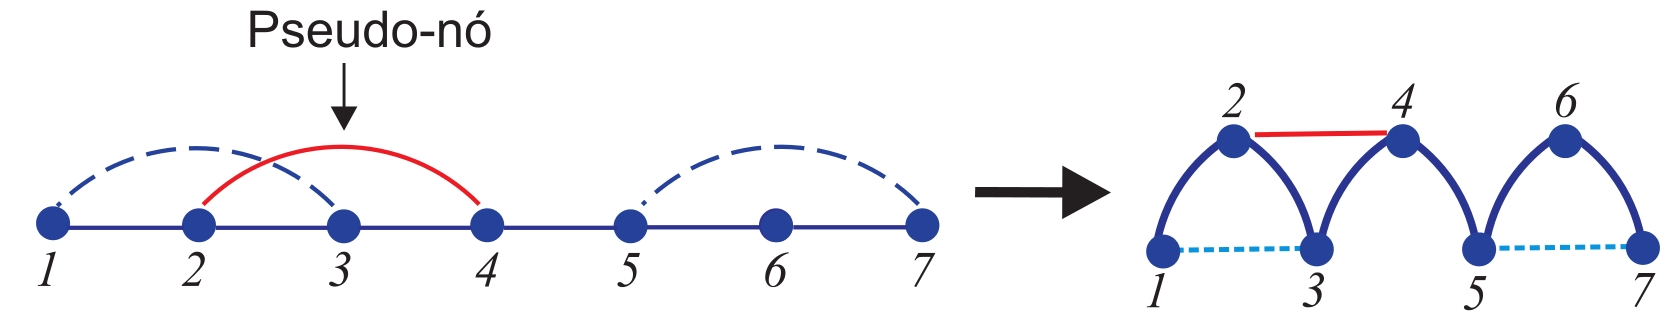
\includegraphics[angle=0,width=1.0\textwidth]{imagens//pseudono.jpg}
%\caption{Pseudo-nó (arco com linha contínua)
% - Um pseudo-nó do RNA consiste em
%um par de bases não aninhadas entre um laço de uma haste e resíduos fora desta haste
%~\citep{eddy2004rna:2004}. \label{fig:pseudono}}
%\end{figure}


\subsubsection{Proposta de Três Principais Abordagens}

Propomos uma classificação dos métodos computacionais para detecção de ncRNAs em três grupos~\citep{griffiths2007annotating:2007,Stadler:2011}:


\textbf{Homologia} \\


Predição de ncRNAs feita por meio de comparação de genomas entre duas ou mais espécies. Essas comparações dependem de bancos de dados curados, no sentido de que quanto melhores forem as anotações do banco melhores serão as predições~\citep{machado2008computational:2008}.

Dois genes são ditos homólogos se descendem de um ancestral comum, e possivelmente esses genes mantenham a mesma funcionalidade herdada. Sequências homólogas podem ser divididas em duas classes: ortólogas e parálogas. As ortólogas são sequências relacionadas por especiação, possuindo uma descendência vertical, já as parálogas são sequências relacionadas por duplicação dentro da mesma espécie ou nos ancestrais~\citep{stryer:2002}.




Duas ferramentas importantes para inferir homologia que usam como métrica similaridade de sequências (quanto maior a similaridade entre duas sequências, maior a chance delas terem herdado a mesma função) são: BLAST~\citep{altschul1990basic:1990}, uma ferramenta para detecção de ncRNAs baseada em alinhamento par a par  entre as estruturas primárias das sequências; e o Infernal~\citep{altschul1990basic:1990}, uma ferramenta baseada em alinhamento múltiplo que considera as estruturas secundárias das sequências. O BLAST em geral não produz bons resultados, sendo O Infernal mais sensível e específico para pesquisar ncRNAs~\citep{eddy2003infernal:2003}.\\


%Duas ferramentas importantes para tentar identificar a homologia por similaridade de sequências, ou seja, quanto maior a similaridade entre duas sequências, maior a chance delas terem herdado a mesma função, são o BLAST~\citep{altschul1990basic:1990}, uma ferramenta para detecção de ncRNAs baseadas em homologia que considera as estruturas primárias das sequências; e o Infernal ~\citep{altschul1990basic:1990}, que considera as estruturas secundárias das sequências. O BLAST, em geral não produz bons resultados para detecção de ncRNAs. O Infernal é mais sensível e específico para pesquisar ncRNAs~\citep{eddy2003infernal:2003}.\\

 %principais que representam a homologia são o BLAST~\citep{altschul1990basic:1990}, embora ele considere a estrutura primária da sequência; e o Infernal ~\citep{altschul1990basic:1990}, o BLAST não produz bons resultados para buscar por RNAs homólogos em bases de dados de sequências de ácidos nucléicos. O Infernal é mais sensível e específica para pesquisa de RNAs homólogos~\citep{eddy2003infernal:2003}.\\


\textbf{Predição de Classe} \\

Predição de ncRNAs feita por métodos de aprendizagem de máquina.

No aprendizado supervisionado, pode-se tomar um conjunto conhecido de ncRNAs e um conjunto conhecido de proteínas, calculando características {\it ab initio} dessas sequências, visando criar um modelo de predição de ncRNAs. Isso confere ao modelo maior confiabilidade.

Por exemplo, o SVM-PORTRAIT~\citep{Arrial:2006,arrial2009screening:2009} mostra um grau de acurácia elevado para sequências de transcritomas ainda não totalmente caracterizadas.\\


%Por exemplo, no aprendizado supervisionado toma-se um conjunto conhecido de ncRNAs, e um conjunto conhecido de proteínas das sequências, a predição de ncRNAs pode ser feita com maior confiabilidade, e usando \textit{ab initio}. Por exemplo, o SVM-PORTRAIT~\citep{Arrial:2006} que mostra um grau de acurácia elevado.\\




% sua estrutura secundária pode ser predita com maior confiabilidade, pois conservação de domínios estruturais em diferentes espécies constitui evidência adicional de que esses domínios estão relacionados com a função específica destas sequências. Com isso, estruturas conservadas são úteis para descobrir e caracterizar assinaturas de uma família específica de RNAs, e podem ser utilizadas para classificar um RNA como membro de uma família comparando sua estrutura com a estrutura das várias famílias conhecidas.

%Métodos que utilizam aprendizado de máquina mostraram um grau de acurácia elevado, como o SVM-PORTRAIT~\citep{Arrial:2006}. \\


\textbf{Modelos \textit{De Novo}} \\

Predição de nRNAs feita por outros modelos, diferentes de {\it homologia} e {\it predição de classe}.

Por exemplo, no modelo termodinâmico, a composição e ordenação de nucleotídeos em uma molécula de RNA é responsável por sua conformação espacial. Uma investigação dessa conformação, por sua vez, resulta em um conhecimento aproximado tanto sobre a organização da molécula quanto sobre suas propriedades fisiológicas. A avaliação termodinâmica de moléculas de RNA pode ser utilizada em conjunto com regras estruturais e topológicas para inferir a estrutura secundária ativa da molécula de RNA~\citep{zuker1981optimal:1981}. 


Um RNA com uma estrutura secundária bem definida tem energia livre associada menor do que sequências com a mesma frequência de nucleotídeos, porém sem estrutura secundária definida~\citep{machado2008computational:2008}. A partir da análise da energia livre mínima de uma molécula de RNA, é possível inferir se ela tem uma conformação de estrutura secundária estável.


%O modelo \textit{De Novo}~\citep{griffiths2007annotating:2007} (inclui outros modelos, como o termodinâmico) pesquisas em transcritômica tem se beneficiado imensamente com o advento das estratégias de sequenciamento de alto desempenho. Sem a necessidade do emprego de técnicas de clonagem, as modernas plataformas  comerciais de sequenciamento podem sequenciar diretamente DNA complementar (cDNA) ou o RNA mensageiro (RNAm) em larga escala.

%Com isso novos algoritmos e técnicas são necessários para analisar e
%classificar as sequências geradas pelas novas plataformas de sequenciamento, 
%surgindo assim o \textit{De Novo}, que tem como objetivo melhorar a acurácia
%e diminuir as deficiências dos métodos anteriores. 
 % cap 3

  \chapter{Sistema Multiagentes e Regras de Inferência}
\label{sec:SistMult}

Neste capítulo, será feita uma breve descrição de Sistemas MultiAgentes. Na Seção \ref{sec:Agent}, falaremos sobre Agentes. A Seção \ref{sec:SMA} detalha conceitos de Sistemas MultiAgentes. A Seção \ref{sec:FerramentaSMA} descreve ferramentas analisadas nesse trabalho. Por fim, na Seção, \ref{sec:RegraInfer}, serão mostrados motores de inferência para raciocínio automático utilizado nesse trabalho.

\subsection{Agentes} \label{sec:Agent}

\begin{figure}[htb!]
\centering
%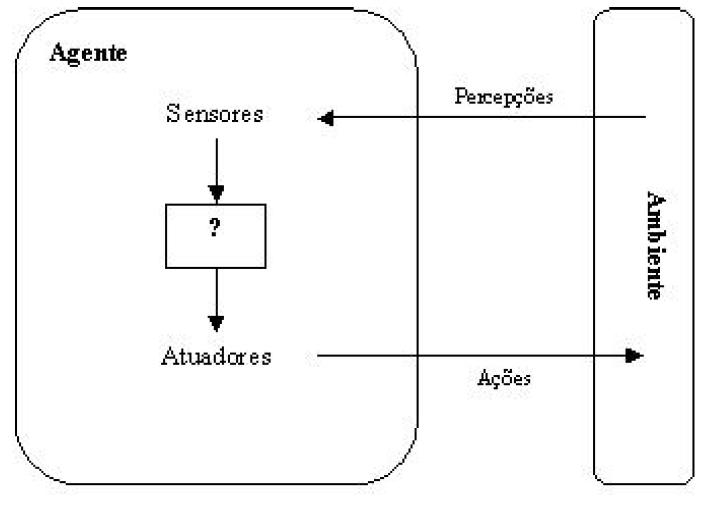
\includegraphics[angle=0,width=0.6\textwidth]{imagens//agentes.JPG}
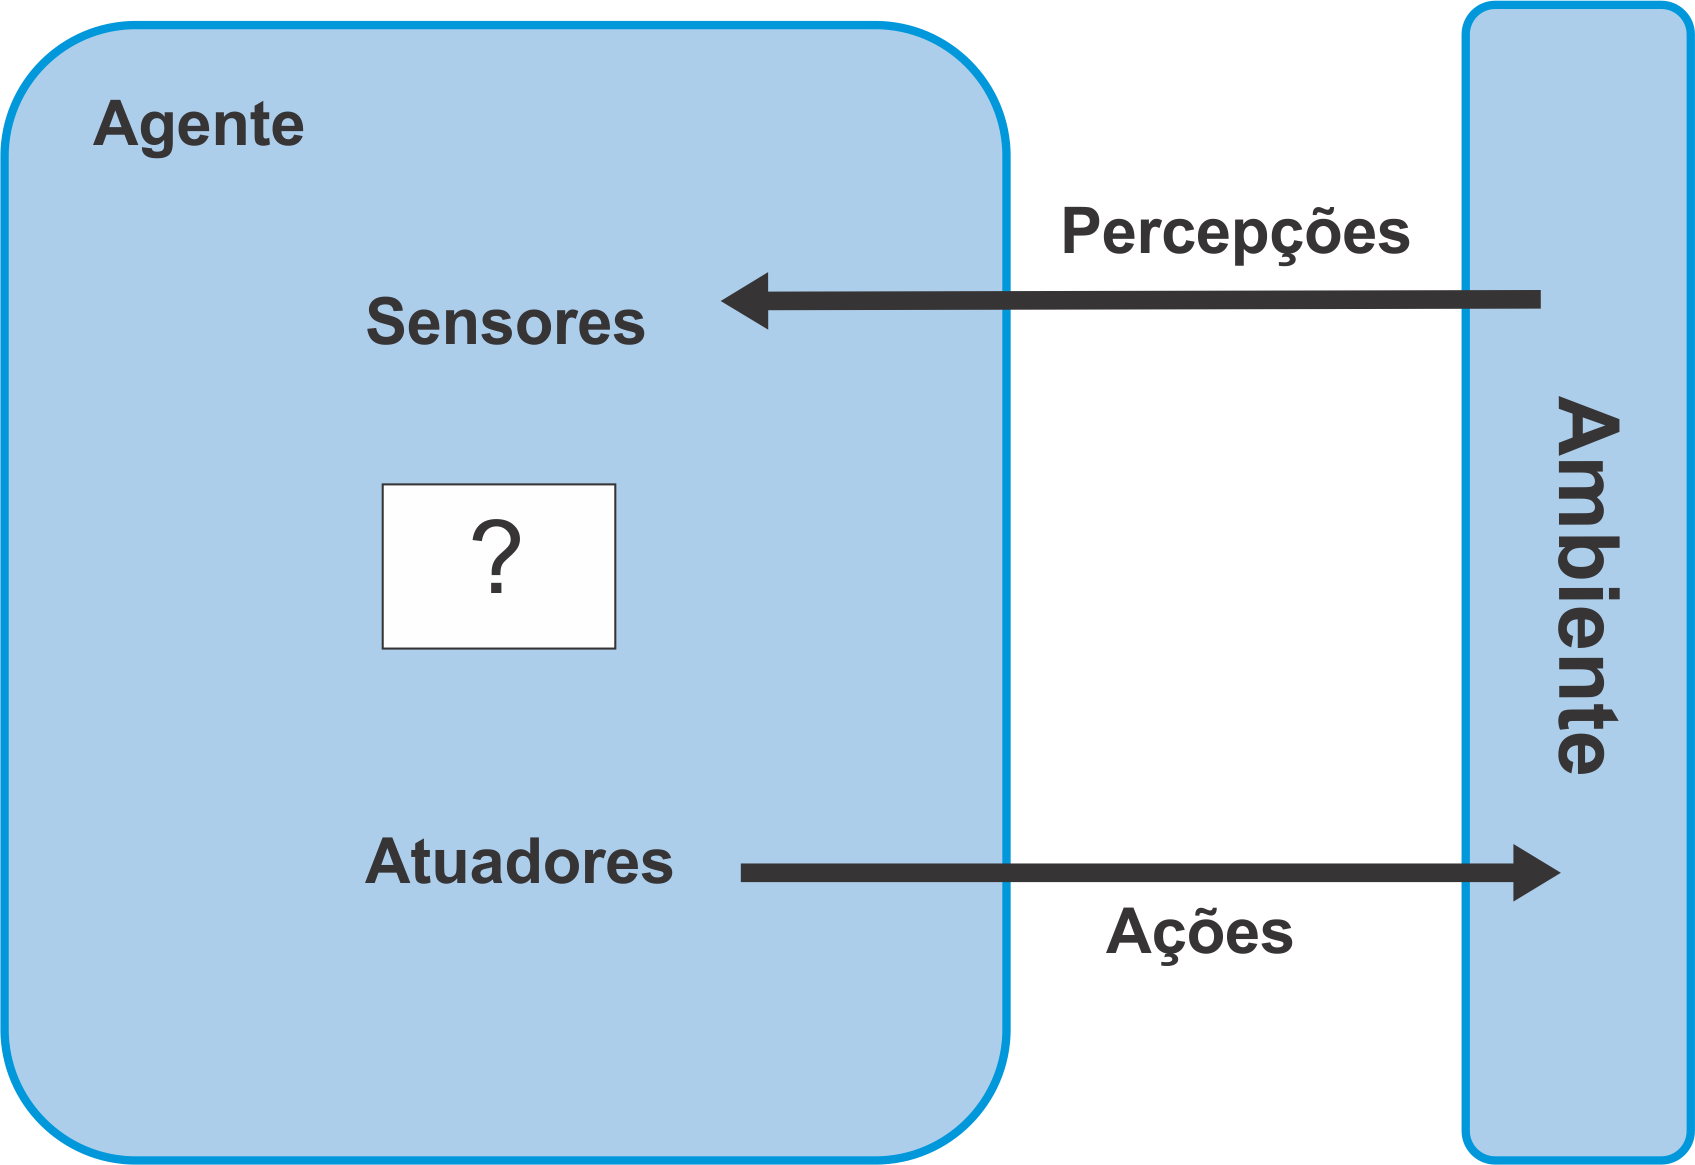
\includegraphics[angle=0,width=0.6\textwidth]{imagens//Agentes1sem.png}
\caption{Arquitetura de um agente inteligente (Adaptado de~\citep{Russell:2002}).} \label{fig:Agente}
\end{figure}


Um agente~\citep{Russell:2002} é uma entidade capaz de perceber seu ambiente através de sensores e de agir sobre esse ambiente através de atuadores Figura~\ref{fig:Agente}. Cada agente exibe duas características fundamentais: é capaz de agir de forma autônoma tomando decisões que levam à satisfação dos seus objetivos; e é capaz de interagir com outros agentes utilizando protocolos de interação social inspirados nos humanos e incluindo pelo menos algumas das seguintes funcionalidades - coordenação, cooperação, competição e negociação~\citep{Russell:2002}.

\subsection{SMAs} \label{sec:SMA}

\begin{figure}[htb!]
\centering
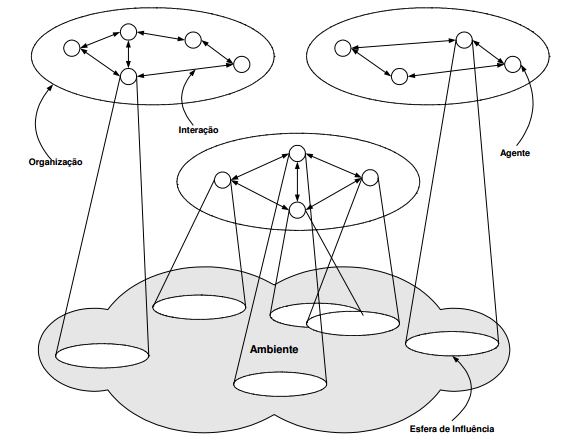
\includegraphics[angle=0,width=0.7\textwidth]{imagens//multiAgent.png}
\caption{Estrutura de um Sistema Multi-Agente (Adaptado de~\citep{wooldridge2009introduction:2009}).} \label{fig:MultiAgent}
\end{figure}

Os Sistemas MultiAgente (SMAs) incluem diversos agentes que interagem ou trabalham em
conjunto, podendo compreender agentes homogêneos ou heterogêneos. Cada agente opera
assincronamente com respeito aos outros agentes~\citep{wooldridge2009introduction:2009}. Para que um agente possa operar como parte do sistema, é necessária a existência de uma infraestrutura que permita a
comunicação e/ou interação entre os agentes que compõem o SMA Figura~\ref{fig:MultiAgent}.

\subsection{Ferramentas para SMAs} \label{sec:FerramentaSMA}

Nesta seção, inicialmente descreveremos ferramentas para a construção de SMAs e em seguida faremos uma comparação entre elas.

\subsubsection{Descrição das Ferramentas}

\subsubsection*{Breve}

É uma ferramenta livre, que permite uma criação de sistemas multiagentes 3D. Ela utiliza como linguagem de programação o Python, ou uma linguagem de \textit{script} com o nome de Steve, ela permite definir comportamentos dos agentes em um mundo 3D e observar como eles interagem. 

\subsubsection*{Cormas}

É uma ferramenta livre, um framework de simulação baseado em agentes. Ela utiliza como linguagem de programação o Visual Works, que permite desenvolver para o SmallTalk, sendo orientada a objeto.   

\subsubsection*{JADE}

O JADE (\textit{Java Agent DEvelopment Framework})~\citep{Bellifemine:2003} segue os padrões da FIPA (Foundation for Intelligent Physical Agents),  uma organização responsável por especificar padrões para o desenvolvimento de tecnologias baseadas em agentes inteligentes. O JADE possibilita e facilita a programação de agentes inteligentes usando Java, possui muitos atributos e características que a tornam ideal para a implementação de agentes, além de simplificar o desenvolvimento por disponibilizar um \textit{framework} que trata a comunicação, o ciclo de vida do agente e o monitoramento da execução, entre outras.

\subsubsection*{Jadex}

É um pacote construído para permitir o desenvolvimento de agentes de acordo com a FIPA e a arquitetura BDI de agentes. JADEX permite a construção de agentes de software seguindo os conceitos do modelo BDI (Belief Desire Intention);

\begin{itemize}
\item [i)] Usa tecnologias como XML e Java;
\item [ii)] JADEX é projetado para facilitar a implementação de agentes em Java, e, portanto permite o reuso de várias ferramentas e bibliotecas.
\end{itemize}
	Um agente JADEX é também um agente JADE e, portanto todas as ferramentas disponíveis em JADE podem ser usadas também para desenvolver agentes em JADEX. A maior parte da plataforma JADE lida com a visão externa de um agente, que não difere entre um agente JADE ou JADEX.

\subsubsection*{Zeus}

É um ambiente integrado para a construção rápida de aplicações com agentes colaborativos. A documentação da ferramenta Zeus é abundante, e coloca uma forte ênfase na importância da metodologia aspecto de Zeus ("A metodologia de criação do agente é vital para o uso do Zeus"). A metodologia de Zeus usa a decomposição de quatro estágios para o mesmo desenvolvimento de agente como em nossa análise, respectivamente análise de domínio, design, realização e apoio a execução.

\subsubsection*{JAS} 

É uma ferramenta em Java para a simulação de agentes. Possui um mecanismo de tempo para eventos discretos, com sondas estáticas embutidas, redes neurais e algoritmos genéticos.

 
\subsubsection*{MADKIT}

É uma ferramenta livre modular e uma plataforma escalave para multiagetens. Ferramenta que trabalha com Java e foi escrito em Java.   

 
\subsubsection*{JASON}

É uma maneira rápida de eventos discretos multiagentes que tem um núcleo com biblioteca de simulação em Java, projetado para ser a base para grandes simulações personalizadas, e também para fornecer mais funcionalidade com suficiência para simulação. MASON contém uma biblioteca de modelo e um conjunto opcional de ferramentas de visualização em 2D e 3D.

\subsubsection*{MicrosoftAgent}

É um conjunto de serviços programável por software que suporta a apresentação dos personagens animados interativos. Os desenvolvedores podem usar personagens como assistentes interativos para apresentar, orientar, entreter, ou melhorar as suas páginas Web ou aplicações além do uso convencional de janelas, menus e controles.

\subsubsection*{NetLogo}

É um ambiente de multi-agente livre com modelagem programável. Ele é usado por dezenas de milhares de estudantes, professores e pesquisadores do mundo todo. É de autoria de Uri Wilensky e desenvolvido no CCL.  


\subsubsection*{Open Architecture Agent (OAA)}

É uma ferramenta focada na construção de comunidades distribuídas de agentes, onde o agente é definido como qualquer processo de software que atenda as convenções da sociedade OAA. Um agente satisfaz este requisito, registrando os serviços que ela pode fornecer em uma forma aceitável, por ser capaz de falar a linguagem de comunicação interagente (ICL), e através da partilha de funcionalidades comuns a todos os agentes OAA. 

\subsubsection*{AgentBuilder}

É um conjunto de ferramentas integradas para a construção de software de agentes inteligentes. É desenvolvido pela Reticular Systems Inc., e está fundamentada no modelo de Agents BDI. Esta ferramenta é notável tanto pela alta qualidade dos seu software e do modelo conhecido.


\subsubsection*{Shell for Simulated Agent Systems (SeSAM)} 

SESAM (Shell para Sistemas de Agente simulado)~\citep{Sesam:2011} fornece um ambiente genérico para modelagem e experimentação de agente baseado em simulação. Está especialmente voltada ao fornecimento de uma ferramenta para a construção fácil de modelos complexos, que incluem interdependências dinâmica ou comportamento emergente. 

\subsubsection*{SIM Agent}

É uma ferramenta com uma gama de recursos para pesquisa e ensino relacionadas com o desenvolvimento de agentes que interagem em ambientes de diferentes graus e tipos de complexidade. Pode ser executado como uma ferramenta de simulação pura. Ela foi originalmente desenvolvida para suportar uma pesquisa exploratória sobre humano, como agentes inteligentes, mas também tem sido usado para projetos de estudantes a desenvolver uma variedade de jogos e simulações interativas.

\subsubsection*{Simulation of Cognitive Agents (SimCog)}

É uma plataforma genérica para SMA de simulação baseada em agentes cognitivos. Ele começou em 2001, no Departamento de Informática da Universidade de Lisboa.

\subsubsection*{StartLogo}

É um ambiente de modelagem programável para explorar o funcionamento de sistemas descentralizados. Sistemas que são organizados sem um gerente, coordenado sem um gerenciador. Com StarLogo, você pode modelar, muitos fenômenos da vida real, como bandos de aves, os engarrafamentos, colônias de formigas, e economias de mercado.

\subsubsection*{Swarm} 

Swarm é uma plataforma para os modelos baseados em agentes - MBA, que inclui:

\begin{itemize}
\item Um framework conceitual para projetar, descrever e conduzir experimentos em MBA;
\item implementação de software com diversas ferramentas úteis, e 
\item uma comunidade de usuários e desenvolvedores que compartilham idéias, softwares e experiências.
\end{itemize}

\subsubsection*{Cougaar}

O Cougaar (\textit{Cognitive Agent Architecture})~\citep{Cougar:2011}, uma plataforma de desenvolvimento de aplicações baseadas em agentes, foi implementada em linguagem Java e disponibiliza uma plataforma \textit{opensource} flexível para o desenvolvimento de aplicações baseadas em agentes de diferentes tipos.

\subsubsection*{JAMA}

O JAMA~\citep{Leone:2011}, escrito em linguagem JAVA, simplifica a construção de aplicações que exploram o conceito de agentes. Possui alto grau de desacoplamento de agentes e utiliza uma rede \textit{peer-to-peer} que garante escalabilidade, descentralização e tolerância a falhas.

%\subsubsection{Comparações das ferramentas} \label{sec:AnexoFerram}


\subsubsection{Descrição dos Critérios de Avaliação} 

Os critérios de avaliação aqui selecionados estão diretamente relacionados com o objetivo em que nossa opinião, no mínimo, deve-se reunir para ser considerada uma boa ferramenta de SMA. Obviamente, as ferramentas aqui avaliadas não são todos os ambientes de desenvolvimento SMA conhecidos na literatura. Algumas podem, possivelmente, obter uma melhor avaliação de acordo essa análise feita por nós. No entanto, não vão satisfazer nosso problema perfeitamente, mas podem satisfazer perfeitamente o objetivo original para qual foram criadas. Os objetivos essenciais do desenvolvimento de ambientes são:


\begin{itemize}
\item Acelerar o desenvolvimento, reduzindo o esforço da programação;
\item Controlar a comunicação, interação e coordenação de mecanismos;
\item Permitir a implementação de sistemas relativamente complexos;
\item Permitir extensibilidade de código simples;
\item Fornecer apoio para a implantação e execução dos sistemas. 
\end{itemize}

\subsection*{Escala de Avaliação} 

A escala utilizada visa atribuir, para cada ferramenta, um número variando entre 0 e 4, interpretados da seguinte forma: 
\begin{itemize}
\item 4, se a ferramenta atende o critério correspondente muito bem;
\item 3, se a ferramenta atende o critério correspondente bem;
\item 2, se a ferramenta atende o critério correspondente moderadamente; 
\item 1, se a ferramenta atende o critério um pouco;
\item 0, se a ferramenta não atende o critério correspondente. 
\end{itemize}

\subsubsection{Definição dos Critérios de Avaliação} 

\begin{enumerate}
\item \textbf{A metodologia atende às diferentes etapas do desenvolvimentos} - A metodologia abrange as várias fases do processo de desenvolvimento. A maioria dos autores consideram que o processo de desenvolvimento de sistemas multiagentes, consiste em quatro etapas principais: Análise, desenvolvimento, implementação e execução (implantação). Muitas vezes podemos ter essa metodologia fracamente acoplada em algumas ferramentas.

\item \textbf{Facilidade de aprendizagem} - Este critério é determinado em função de vários fatores, como a qualidade da documentação, a complexidade dos componentes e a clareza dos conceitos utilizados. O conhecimento necessário para utilizar corretamente a ferramenta, incluindo a linguagem de programação, a linguagem de comunicação entre os agentes e o protocolo de interação.

\item \textbf{Transição entre o desenvolvimento e a aplicação é simples} - Facilidade para passar do modelo para a sua implementação várias metodologias desenvolvidas são muito interessantes a nível conceitual, mas não são facilmente aplicável, olhando pelo lado dos detalhes da implementação .

\item \textbf{Flexibilidade da ferramenta  para o desenvolvimento} - Flexibilidade da ferramenta é a versatilidade para o uso dos seus componentes e a sua metodologia. 

\item \textbf{Comunicação entre os Agentes} - O programador não deveria ter que se preocupar com a implementação de conexões de baixo nível entre vários computadores, protocolos de comunicação, gerenciamento de segurança, sincronização, serviços de transporte de mensagens e assim por diante. Este serviço deve ser já implementado ao desenvolver.  

\item \textbf{Método de Depuração} - Vários erros de coordenação e sincronização podem acontecer quando está se programando durante o desenvolvimento de SMA. A descoberta e correção desses erros podem ser muito difíceis ou mesmo impossíveis sem instrumento adequados de depuração.  


\item \textbf{Apoio Gráfico ao Desenvolvimento e Implementação} - O ambiente propõe interfaces gráficas, facilitando e acelerando o desenvolvimento e implementação. Estes podem ser utilizados para criação de modelos, criação de agentes, desenvolvimento da comunicação entre os agentes, e implantação dos agentes em várias plataformas. 

\item \textbf{Suporte ao Gerenciamento do SMA} - A ferramenta permite a interação com o sistema. Ele permite, por exemplo, adicionar dinamicamente, modificar ou remover agentes no sistema. O interesse deste tipo de gestão é significativo, ele pode ser muito útil para poder estudar o sistema em execução, verificando ou avaliando os níveis.  

\item \textbf{Simplicidade de Implementação e Redução do Esforço necessário} - Com este critério, vários fatores devem ser levados em conta, a linguagem de progamação que a ferramenta suporta, se suporta programação orientada a objeto, muilti-threading e programação em rede, tendo vantagens significativas em detrimento de outros que não. Os componentes devem ser de fácil identificação (nome, documentação, parâmetros, etc). Além disso, as classes e os serviços disponíveis devem ser de fácil uso. A redução do esforço e necessário em termos de quantidade de código, componentes, complexidade de implementação, simplicidade de utilização dos componentes que já existem.


\item \textbf{Suporte ao Uso de Banco de Dados} - Dados de conservação e de proteção é uma tarefa técnica no nível de programação, esse processo é interessante e abstrato tanto como possíveis ferramentas para facilitar.  

\item \textbf{Geração automática de Código} - Facilidade para o progresso do modelo durante sua implementação. Várias metodologias desenvolvidas são muito interessantes a nível conceitual, mas que não são facilmente aplicáveis, levando para o lado da implementação.  

\item \textbf{Extensibilidade do Código} - Utilitários fornecidos pelas ferramentas, como os módulos pré-definidos, agentes ou códigos gerados, devem ser facilmente modificadas. Sendo necessárias para ser capaz de facilmente adicionar o código para as peças existentes no código.

\item \textbf{Suporte ao Desenvolvimento de Sistema Distribuído} - A possibilidade de distribuir o sistema em várias maquinas é um critério muito importante no nível da execução. A ferramenta deve também permitir uma execução simples do sistema. A execução deve ser independente do ambiente. 

\item \textbf{Documentação} - É importante ter uma boa documentação e de boa qualidade, abrangendo todos os componentes da ferramenta. Além disso, é claro, concisa e não ambígua.
\end{enumerate}
 
%\subsection*{A metodologia atende às diferentes etapas do desenvolvimentos (1)}
%\subsection*{Facilidade de aprendizagem (2)}
%\subsection*{Transição entre o desenvolvimento e a aplicação é simples (3)}
%\subsection*{Flexibilidade da Ferramenta  para o desenvolvimento (4)}
%\subsection*{Comunicação entre os Agentes (5)}
%\subsection*{Método de Depuração (6)}
%\subsection*{Apoio Gráfico ao Desenvolvimento e Implementação (7)}
%\subsection*{Suporte ao Gerenciamento do SMA (8)}
%\subsection*{Simplicidade de Implementação e Redução do Esforço necessário (9)}
%\subsection*{Suporte ao Uso de Banco de Dados (10)}
%\subsection*{Geração automática de Código (11)}
%\subsection*{Extensibilidade do Código (12)}
%\subsection*{Suporte ao Desenvolvimento de Sistema Distribuído (13)}
%\subsection*{Documentação (14)}

Outros critérios foram considerados durante essa primeira avaliação comparativa. Entre esses critérios, tivemos a metodologia utilizada para o desenvolvimento, a linguagem de comunicação entre os agentes e a linguagem de programação.  
 
\subsubsection{Compara\c{c}\~ao entre Ferramentas}

Como base na Tabela \ref{tab:CompFerramSMAs}, podemos verificar que a ferramenta JADE conseguiu o melhor resultado na avaliação.

\begin{table}[htb!]
\caption{Avaliação das Ferramentas} \label{tab:CompFerramSMAs}
\begin{tabular}{|l|l|l|l|l|l|l|l|l|l|l|l|l|l|l|l|}
\cline{2-16}
\multicolumn{1}{c|}{} & \multicolumn{15}{c|}{\textbf{Critérios}} \\ 
\hline
\textbf{Ferramentas} & \textbf{1} & \textbf{2} & \textbf{3} & \textbf{4} & \textbf{5} & \textbf{6} & \textbf{7} & \textbf{8} & \textbf{9} & \textbf{10} & \textbf{11} & \textbf{12} & \textbf{13} & \textbf{14} & \textbf{Total} \\ 
\hline
\textbf{Breve} & \multicolumn{1}{c|}{1} & \multicolumn{1}{c|}{1} & \multicolumn{1}{c|}{3} & \multicolumn{1}{c|}{1} & \multicolumn{1}{c|}{4} & \multicolumn{1}{c|}{3} & \multicolumn{1}{c|}{2} & \multicolumn{1}{c|}{3} & \multicolumn{1}{c|}{2} & \multicolumn{1}{c|}{1} & \multicolumn{1}{c|}{1} & \multicolumn{1}{c|}{1} & \multicolumn{1}{c|}{2} & \multicolumn{1}{c|}{4} & \multicolumn{1}{c|}{29} \\ 
\hline
\textbf{Cormas} & \multicolumn{1}{c|}{1} & \multicolumn{1}{c|}{2} & \multicolumn{1}{c|}{3} & \multicolumn{1}{c|}{1} & \multicolumn{1}{c|}{3} & \multicolumn{1}{c|}{4} & \multicolumn{1}{c|}{3} & \multicolumn{1}{c|}{2} & \multicolumn{1}{c|}{3} & \multicolumn{1}{c|}{1} & \multicolumn{1}{c|}{1} & \multicolumn{1}{c|}{1} & \multicolumn{1}{c|}{2} & \multicolumn{1}{c|}{4} & \multicolumn{1}{c|}{31} \\ 
\hline
\textbf{Jade} & \multicolumn{1}{c|}{3} & \multicolumn{1}{c|}{4} & \multicolumn{1}{c|}{2} & \multicolumn{1}{c|}{3} & \multicolumn{1}{c|}{4} & \multicolumn{1}{c|}{4} & \multicolumn{1}{c|}{3} & \multicolumn{1}{c|}{4} & \multicolumn{1}{c|}{2} & \multicolumn{1}{c|}{0} & \multicolumn{1}{c|}{0} & \multicolumn{1}{c|}{4} & \multicolumn{1}{c|}{4} & \multicolumn{1}{c|}{4} & \multicolumn{1}{c|}{41} \\ 
\hline
\textbf{Jadex} & \multicolumn{1}{c|}{0} & \multicolumn{1}{c|}{0} & \multicolumn{1}{c|}{2} & \multicolumn{1}{c|}{3} & \multicolumn{1}{c|}{4} & \multicolumn{1}{c|}{4} & \multicolumn{1}{c|}{0} & \multicolumn{1}{c|}{4} & \multicolumn{1}{c|}{2} & \multicolumn{1}{c|}{0} & \multicolumn{1}{c|}{0} & \multicolumn{1}{c|}{4} & \multicolumn{1}{c|}{4} & \multicolumn{1}{c|}{4} & \multicolumn{1}{c|}{30} \\ 
\hline
\textbf{Zeus} & \multicolumn{1}{c|}{3} & \multicolumn{1}{c|}{1} & \multicolumn{1}{c|}{2} & \multicolumn{1}{c|}{1} & \multicolumn{1}{c|}{4} & \multicolumn{1}{c|}{2} & \multicolumn{1}{c|}{3} & \multicolumn{1}{c|}{3} & \multicolumn{1}{c|}{2} & \multicolumn{1}{c|}{2} & \multicolumn{1}{c|}{3} & \multicolumn{1}{c|}{2} & \multicolumn{1}{c|}{2} & \multicolumn{1}{c|}{4} & \multicolumn{1}{c|}{34} \\ 
\hline
\textbf{JAS} & \multicolumn{1}{c|}{0} & \multicolumn{1}{c|}{0} & \multicolumn{1}{c|}{2} & \multicolumn{1}{c|}{1} & \multicolumn{1}{c|}{2} & \multicolumn{1}{c|}{2} & \multicolumn{1}{c|}{0} & \multicolumn{1}{c|}{2} & \multicolumn{1}{c|}{2} & \multicolumn{1}{c|}{0} & \multicolumn{1}{c|}{0} & \multicolumn{1}{c|}{4} & \multicolumn{1}{c|}{4} & \multicolumn{1}{c|}{4} & \multicolumn{1}{c|}{22} \\ 
\hline
\textbf{Madkit}  & \multicolumn{1}{c|}{3} & \multicolumn{1}{c|}{2} & \multicolumn{1}{c|}{2} & \multicolumn{1}{c|}{3} & \multicolumn{1}{c|}{3} & \multicolumn{1}{c|}{3} & \multicolumn{1}{c|}{0} & \multicolumn{1}{c|}{4} & \multicolumn{1}{c|}{1} & \multicolumn{1}{c|}{0} & \multicolumn{1}{c|}{0} & \multicolumn{1}{c|}{3} & \multicolumn{1}{c|}{3} & \multicolumn{1}{c|}{3} & \multicolumn{1}{c|}{30} \\ 
\hline
\textbf{JASON} & \multicolumn{1}{c|}{2} & \multicolumn{1}{c|}{0} & \multicolumn{1}{c|}{2} & \multicolumn{1}{c|}{1} & \multicolumn{1}{c|}{2} & \multicolumn{1}{c|}{2} & \multicolumn{1}{c|}{0} & \multicolumn{1}{c|}{2} & \multicolumn{1}{c|}{2} & \multicolumn{1}{c|}{0} & \multicolumn{1}{c|}{2} & \multicolumn{1}{c|}{4} & \multicolumn{1}{c|}{4} & \multicolumn{1}{c|}{4} & \multicolumn{1}{c|}{24} \\ 
\hline
\textbf{MicrosoftAgent} & \multicolumn{1}{c|}{3} & \multicolumn{1}{c|}{1} & \multicolumn{1}{c|}{3} & \multicolumn{1}{c|}{1} & \multicolumn{1}{c|}{4} & \multicolumn{1}{c|}{3} & \multicolumn{1}{c|}{3} & \multicolumn{1}{c|}{3} & \multicolumn{1}{c|}{2} & \multicolumn{1}{c|}{1} & \multicolumn{1}{c|}{1} & \multicolumn{1}{c|}{1} & \multicolumn{1}{c|}{2} & \multicolumn{1}{c|}{4} & \multicolumn{1}{c|}{32} \\ 
\hline
\textbf{NetLogo} & \multicolumn{1}{c|}{2} & \multicolumn{1}{c|}{3} & \multicolumn{1}{c|}{2} & \multicolumn{1}{c|}{3} & \multicolumn{1}{c|}{3} & \multicolumn{1}{c|}{3} & \multicolumn{1}{c|}{1} & \multicolumn{1}{c|}{4} & \multicolumn{1}{c|}{1} & \multicolumn{1}{c|}{0} & \multicolumn{1}{c|}{0} & \multicolumn{1}{c|}{3} & \multicolumn{1}{c|}{3} & \multicolumn{1}{c|}{3} & \multicolumn{1}{c|}{31} \\ 
\hline
\textbf{OAA} & \multicolumn{1}{c|}{3} & \multicolumn{1}{c|}{2} & \multicolumn{1}{c|}{2} & \multicolumn{1}{c|}{3} & \multicolumn{1}{c|}{3} & \multicolumn{1}{c|}{3} & \multicolumn{1}{c|}{1} & \multicolumn{1}{c|}{1} & \multicolumn{1}{c|}{3} & \multicolumn{1}{c|}{0} & \multicolumn{1}{c|}{3} & \multicolumn{1}{c|}{3} & \multicolumn{1}{c|}{0} & \multicolumn{1}{c|}{3} & \multicolumn{1}{c|}{30} \\ 
\hline
\textbf{AgentBuilder} & \multicolumn{1}{c|}{2} & \multicolumn{1}{c|}{1} & \multicolumn{1}{c|}{3} & \multicolumn{1}{c|}{1} & \multicolumn{1}{c|}{4} & \multicolumn{1}{c|}{3} & \multicolumn{1}{c|}{3} & \multicolumn{1}{c|}{3} & \multicolumn{1}{c|}{2} & \multicolumn{1}{c|}{1} & \multicolumn{1}{c|}{1} & \multicolumn{1}{c|}{1} & \multicolumn{1}{c|}{2} & \multicolumn{1}{c|}{4} & \multicolumn{1}{c|}{31} \\ 
\hline
\textbf{SeSAM} & \multicolumn{1}{c|}{2} & \multicolumn{1}{c|}{1} & \multicolumn{1}{c|}{2} & \multicolumn{1}{c|}{4} & \multicolumn{1}{c|}{2} & \multicolumn{1}{c|}{2} & \multicolumn{1}{c|}{0} & \multicolumn{1}{c|}{2} & \multicolumn{1}{c|}{2} & \multicolumn{1}{c|}{2} & \multicolumn{1}{c|}{0} & \multicolumn{1}{c|}{4} & \multicolumn{1}{c|}{1} & \multicolumn{1}{c|}{4} & \multicolumn{1}{c|}{26} \\ 
\hline
\textbf{SIM Agent} & \multicolumn{1}{c|}{2} & \multicolumn{1}{c|}{2} & \multicolumn{1}{c|}{3} & \multicolumn{1}{c|}{1} & \multicolumn{1}{c|}{4} & \multicolumn{1}{c|}{3} & \multicolumn{1}{c|}{3} & \multicolumn{1}{c|}{3} & \multicolumn{1}{c|}{2} & \multicolumn{1}{c|}{1} & \multicolumn{1}{c|}{1} & \multicolumn{1}{c|}{1} & \multicolumn{1}{c|}{2} & \multicolumn{1}{c|}{4} & \multicolumn{1}{c|}{32} \\ 
\hline
\textbf{SimCog} & \multicolumn{1}{c|}{0} & \multicolumn{1}{c|}{0} & \multicolumn{1}{c|}{2} & \multicolumn{1}{c|}{1} & \multicolumn{1}{c|}{2} & \multicolumn{1}{c|}{0} & \multicolumn{1}{c|}{2} & \multicolumn{1}{c|}{0} & \multicolumn{1}{c|}{2} & \multicolumn{1}{c|}{0} & \multicolumn{1}{c|}{0} & \multicolumn{1}{c|}{4} & \multicolumn{1}{c|}{4} & \multicolumn{1}{c|}{4} & \multicolumn{1}{c|}{20} \\ 
\hline
\textbf{StartLogo} & \multicolumn{1}{c|}{1} & \multicolumn{1}{c|}{1} & \multicolumn{1}{c|}{2} & \multicolumn{1}{c|}{1} & \multicolumn{1}{c|}{2} & \multicolumn{1}{c|}{2} & \multicolumn{1}{c|}{0} & \multicolumn{1}{c|}{2} & \multicolumn{1}{c|}{2} & \multicolumn{1}{c|}{2} & \multicolumn{1}{c|}{0} & \multicolumn{1}{c|}{4} & \multicolumn{1}{c|}{4} & \multicolumn{1}{c|}{4} & \multicolumn{1}{c|}{25} \\ 
\hline
\textbf{Swarm} & \multicolumn{1}{c|}{2} & \multicolumn{1}{c|}{2} & \multicolumn{1}{c|}{3} & \multicolumn{1}{c|}{1} & \multicolumn{1}{c|}{4} & \multicolumn{1}{c|}{3} & \multicolumn{1}{c|}{3} & \multicolumn{1}{c|}{3} & \multicolumn{1}{c|}{2} & \multicolumn{1}{c|}{1} & \multicolumn{1}{c|}{1} & \multicolumn{1}{c|}{1} & \multicolumn{1}{c|}{2} & \multicolumn{1}{c|}{4} & \multicolumn{1}{c|}{32} \\ 
\hline
\textbf{Cougar} & \multicolumn{1}{c|}{1} & \multicolumn{1}{c|}{1} & \multicolumn{1}{c|}{2} & \multicolumn{1}{c|}{1} & \multicolumn{1}{c|}{3} & \multicolumn{1}{c|}{3} & \multicolumn{1}{c|}{2} & \multicolumn{1}{c|}{2} & \multicolumn{1}{c|}{4} & \multicolumn{1}{c|}{1} & \multicolumn{1}{c|}{2} & \multicolumn{1}{c|}{3} & \multicolumn{1}{c|}{3} & \multicolumn{1}{c|}{2} & \multicolumn{1}{c|}{30} \\ 
\hline
\textbf{JAMA} & \multicolumn{1}{c|}{1} & \multicolumn{1}{c|}{2} & \multicolumn{1}{c|}{1} & \multicolumn{1}{c|}{1} & \multicolumn{1}{c|}{2} & \multicolumn{1}{c|}{1} & \multicolumn{1}{c|}{2} & \multicolumn{1}{c|}{1} & \multicolumn{1}{c|}{1} & \multicolumn{1}{c|}{1} & \multicolumn{1}{c|}{0} & \multicolumn{1}{c|}{1} & \multicolumn{1}{c|}{3} & \multicolumn{1}{c|}{1} & \multicolumn{1}{c|}{18} \\ 
\hline
\end{tabular}

\end{table}


\newpage
\subsection{Motores de Regras de Inferência} \label{sec:RegraInfer}

Como estamos insteresssados na utilização de mecanismos de raciocínio, realizamos levantamento de sistemas que permitem simulação de raciocínio, baseado em informações armazenadas em base de conhecimento.

\subsubsection{Ferramentas}

\subsubsection*{JESS}

O JESS (\textit{Java Expert System Shell})~\citep{friedman2003jess:2003}, criado pela NASA em 1997, é considerado o primeiro produto de software cujo objetivo é integrar os objetos de um sistema Orientado a Objetos (OO) com regras de domínio. O JESS é um software para criação de sistemas baseados em regras e foi utilizado em
sistemas construídos com as linguagens de programação C e C++.

Seu motor de inferência utiliza o algoritmo RETE~\citep{forgy1982rete:1982}. O JESS é
na verdade uma interface para comandos (\textit{shell}), no qual os comandos são utilizados
em uma linguagem própria que, além de permitir a criação de \textit{scripts} de regras de
interpretação, possibilita que os objetos Java sejam utilizados como ligações para os
fatos do contexto.


\subsubsection*{Drools}

O Drools~\citep{Browne:2009} é um motor para construção de bases de conhecimento e de inferência dirigida por padrões. Foi construído para interagir com Java e o conhecimento é obtido das suas regras declarativas. Uma regra Drools tem uma ou mais condições (ou fatos) que levam a uma ou mais ações (ou consequências).

Basicamente, o motor de inferência do Drools oferece a possibilidade de utilização do método de "encadeamento para frente" e do método de "encadeamento para trás" como abordagem de investigação. O algoritmo de inferência presente no Drools é o RETE~\citep{friedman2003jess:2003}, como no JESS, é adaptado para sistemas orientados a objetos.


\subsubsection*{Hammurapi Rules}

\textit{Hammurapi Rules}~\citep{Hammurapi:2012} é um software desenvolvido em Java, cuja principal
idéia, segundo seus desenvolvedores (\textit{Hammurapi Group}), é a de apoiar o
desenvolvimento de sistemas baseados em regras de uma maneira mais simples e
rápida.

O motor de inferência do \textit{Hammurapi Rules}~\citep{Hammurapi:2012} oferece a possibilidade de
utilização dos dois métodos tradicionais de investigação, o "encadeamento para frente" e o "encadeamento para trás", com a implementação do tradicional algoritmo de inferência RETE~\citep{forgy1982rete:1982}, como no JESS e no Drools.

O Hammurapi Rules permite utilizar a própria linguagem Java para escrita das regras e, consequentemente, os próprios objetos do domínio. No Hammurapi Rules os operadores presentes na
linguagem Java são os responsáveis por descrever as relações e condições presentes nas
regras.

\subsubsection{Defini\c{c}\~ao dos Crit\'erios de Avalia\c{c}\~ao}

\begin{enumerate}
\item \textbf{Integra\c{c}\~ao com a linguagem de programa\c{c}\~ao} - Os tr\^es produtos apresentam algum tipo de rela\c{c}\~ao com a linguagem Java. \'E pass\'ivel de uma explica\c{c}\~ao o fato de que o Drools e o JESS n\~ao tenham obtido a classifica\c{c}\~ao m\'axima ("PRESENTE"). Ambos t\^em prop\'ositos um pouco mais gerais do que o
Hammurapi Rules. Em vista disso, o Drools e o JESS abdicam de um compromisso maior com a integra\c{c}\~ao, buscando uma maior abrang\^encia de apoio no desenvolvimento. O JESS e o Drools auxiliam a cria\c{c}\~ao de sistemas baseados em regras em Java, mas s\'o a experi\^encia na linguagem de programa\c{c}\~ao n\~ao \'e suficiente para o
processo de desenvolvimento.

\item \textbf{Monitora\c{c}\~ao autom\'atica do contexto} - No JESS, a monitora\c{c}\~ao do contexto est\'a presente, por meio da rela\c{c}\~ao entre os objetos do dom\'inio e o contexto. O JESS oferece uma monitora\c{c}\~ao autom\'atica com base na abordagem de "monitora\c{c}\~ao por eventos", na qual sempre que os objetos do dom\'inio alteram, as regras s\~ao investigadas. No caso do JESS, todas as regras s\~ao investigadas sempre que um dos objetos do dom\'inio sofre altera\c{c}\~ao. A vantagem computacional associada \`a monitora\c{c}\~ao por eventos n\~ao parece ser importante, pelo menos sob este aspecto. No Drools, a monitora\c{c}\~ao autom\'atica pode vir a ter melhor desempenho que o JESS, mesmo adotando a abordagem de "monitora\c{c}\~ao peri\'odica". O n\'umero de regras e o dom\'inio do sistema ser\~ao determinantes para uma poss\'ivel medida de desempenho entre as duas abordagens.

\item \textbf{Express\~ao de regras de primeira ordem} - Desconsiderando o n\'umero de operadores, pode-se afirmar que a express\~ao do conhecimento por meio de regras de primeira ordem est\'a presente nos tr\^es produtos.

\item \textbf{Express\~ao de regras de segunda ordem ou temporais} - As regras de segunda ordem ou temporais s\'o est\~ao presentes no Drools. 
\end{enumerate}


\subsubsection{Análise dos Crit\'erios de Avalia\c{c}\~ao} \label{sec:DescAvaliMoteres}


Os crit\'erios avalia\c{c}\~ao foram estabelecidos para formalizar de maneira adequada a simula\c{c}\~ao do racioc\'inio dos bi\'ologos no ncRNA-Agents. A análise desses crit\'erios, foi definida em termos de:

\begin{itemize}
\item aus\^encia do recurso: AUSENTE;
\item presen\c{c}a parcial do recurso: PARCIALMENTE;
\item presen\c{c}a completa do recurso: PRESENTE;
\end{itemize}

Posto isso, neste trabalho \'e considerado para integra\c{c}\~ao com a linguagem de programa\c{c}\~ao: como presente,  (PRESENTE) se o produto oferecer uma maneira de implementar as regras por meio dos pr\'oprios objetos JAVA, sem \textit{scripts} intermedi\'arios; no caso de parcial (PARCIALMENTE), o produto oferece uma maneira de implementar as regras por meio dos pr\'oprios objetos JAVA, com scripts intermedi\'arios; foi tratado como ausente (AUSENTE) o caso do produto n\~ao ofere\c{c}a nenhuma maneira de implementar as regras por meio dos pr\'oprios objetos JAVA.


Al\'em disso, para a monitora\c{c}\~ao do contexto foi considerado: Como presente (PRESENTE) se o produto oferecer as duas maneiras mencionadas de monitora\c{c}\~ao autom\'atica, sendo: monitora\c{c}\~ao peri\'odica e monitora\c{c}\~ao por eventos; como parcial (PARCIALMENTE) se o produto oferecer pelo menos uma das
duas maneiras mencionadas de monitora\c{c}\~ao autom\'atica - monitora\c{c}\~ao peri\'odica ou monitora\c{c}\~ao por eventos; foi tratado como ausente (AUSENTE), o caso do produto n\~ao oferecer pelo menos uma das duas maneiras mencionadas de monitora\c{c}\~ao autom\'atica - monitora\c{c}\~ao peri\'odica ou monitora\c{c}\~ao por eventos. 

\subsubsection{Comparação de Motores de Inferência}

A Tabela \ref{tab:CompFerram} traz uma comparação entre os motores de inferência, mostrando o Drools com o melhor resultado para os critérios propostos.

%\begin{table}[ht]
%\caption{Comparação entre Motores de Inferência.} \label{tab:CompFerram}
%\centering
%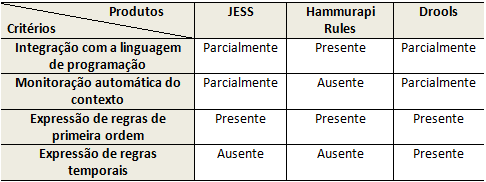
\includegraphics[angle=0,width=0.9\textwidth]{imagens//CompFerram.png}
%\end{table}

\begin{table}[ht]
\caption{Avaliação dos Motores de Inferência.} \label{tab:CompFerram}
\centering
\begin{tabular}{|l|l|l|l|}
\cline{2-4}
\multicolumn{1}{l|}{} & \multicolumn{3}{c|}{\textbf{Produtos}} \\ 
\hline
\textbf{Critérios} & \multicolumn{1}{c|}{\textbf{JESS}} & \multicolumn{1}{c|}{\textbf{Hummurapi} } & \multicolumn{1}{c|}{\textbf{Drools}} \\ 
 & \multicolumn{1}{c|}{} & \multicolumn{1}{c|}{\textbf{Rules}} & \multicolumn{1}{c|}{} \\ 
\hline
\multicolumn{1}{|c|}{\textbf{Integração com linguagem}} & \multicolumn{1}{c|}{Parcialmente} & \multicolumn{1}{c|}{Presente} & \multicolumn{1}{c|}{Parcialmente} \\ 
\multicolumn{1}{|c|}{\textbf{de programação}} & \multicolumn{1}{c|}{} & \multicolumn{1}{c|}{} & \multicolumn{1}{c|}{} \\ 
\hline
\multicolumn{1}{|c|}{\textbf{Monitoração automática do}} & \multicolumn{1}{c|}{Parcialmente} & \multicolumn{1}{c|}{Ausente} & \multicolumn{1}{c|}{Parcialmente} \\ 
\multicolumn{1}{|c|}{\textbf{contexto}} & \multicolumn{1}{c|}{} & \multicolumn{1}{c|}{} & \multicolumn{1}{c|}{} \\ 
\hline
\multicolumn{1}{|c|}{\textbf{Expressão de regras de}} & \multicolumn{1}{c|}{Presente} & \multicolumn{1}{c|}{Presente} & \multicolumn{1}{c|}{Presente} \\ 
\multicolumn{1}{|c|}{\textbf{primeira ordem}} & \multicolumn{1}{c|}{} & \multicolumn{1}{c|}{} & \multicolumn{1}{c|}{} \\ 
\hline
\multicolumn{1}{|c|}{\textbf{Expressão de regras}} & \multicolumn{1}{c|}{Ausente} & \multicolumn{1}{c|}{Ausente} & \multicolumn{1}{c|}{Presente} \\ 
\multicolumn{1}{|c|}{\textbf{temporais}} & \multicolumn{1}{c|}{} & \multicolumn{1}{c|}{} & \multicolumn{1}{c|}{} \\ 
\hline
\end{tabular}
\end{table} % cap 4

  \chapter{Projeto: ncRNA-Agents}
\label{sec:propostaNcRNAs}

Neste capítulo, apresentamos a arquitetura de um sistema de anota\c{c}\~ao de ncRNAs baseado em SMAs. Na Se\c{c}\~ao \ref{sec:ArqAnotacao}, apresentaremos a arquitetura adotada no sistema ncRNA-Agents. Na Se\c{c}\~ao \ref{sec:Implemetacao}, serão apresentandos os detalhes da implementa\c{c}\~ao do ncRNA-Agents.


\subsection{Arquitetura} \label{sec:ArqAnotacao}

Observamos que o presente projeto foi inspirado no trabalho de Ralha e 
co-autores~\citep{Schneider2006:2006,Ralha2011:2011}, que propuseram um sistema para anotação baseado em SMAs, denominado BioAgents Figura \ref{fig:441}.

\begin{landscape}
\begin{figure}[htb!]
\centering
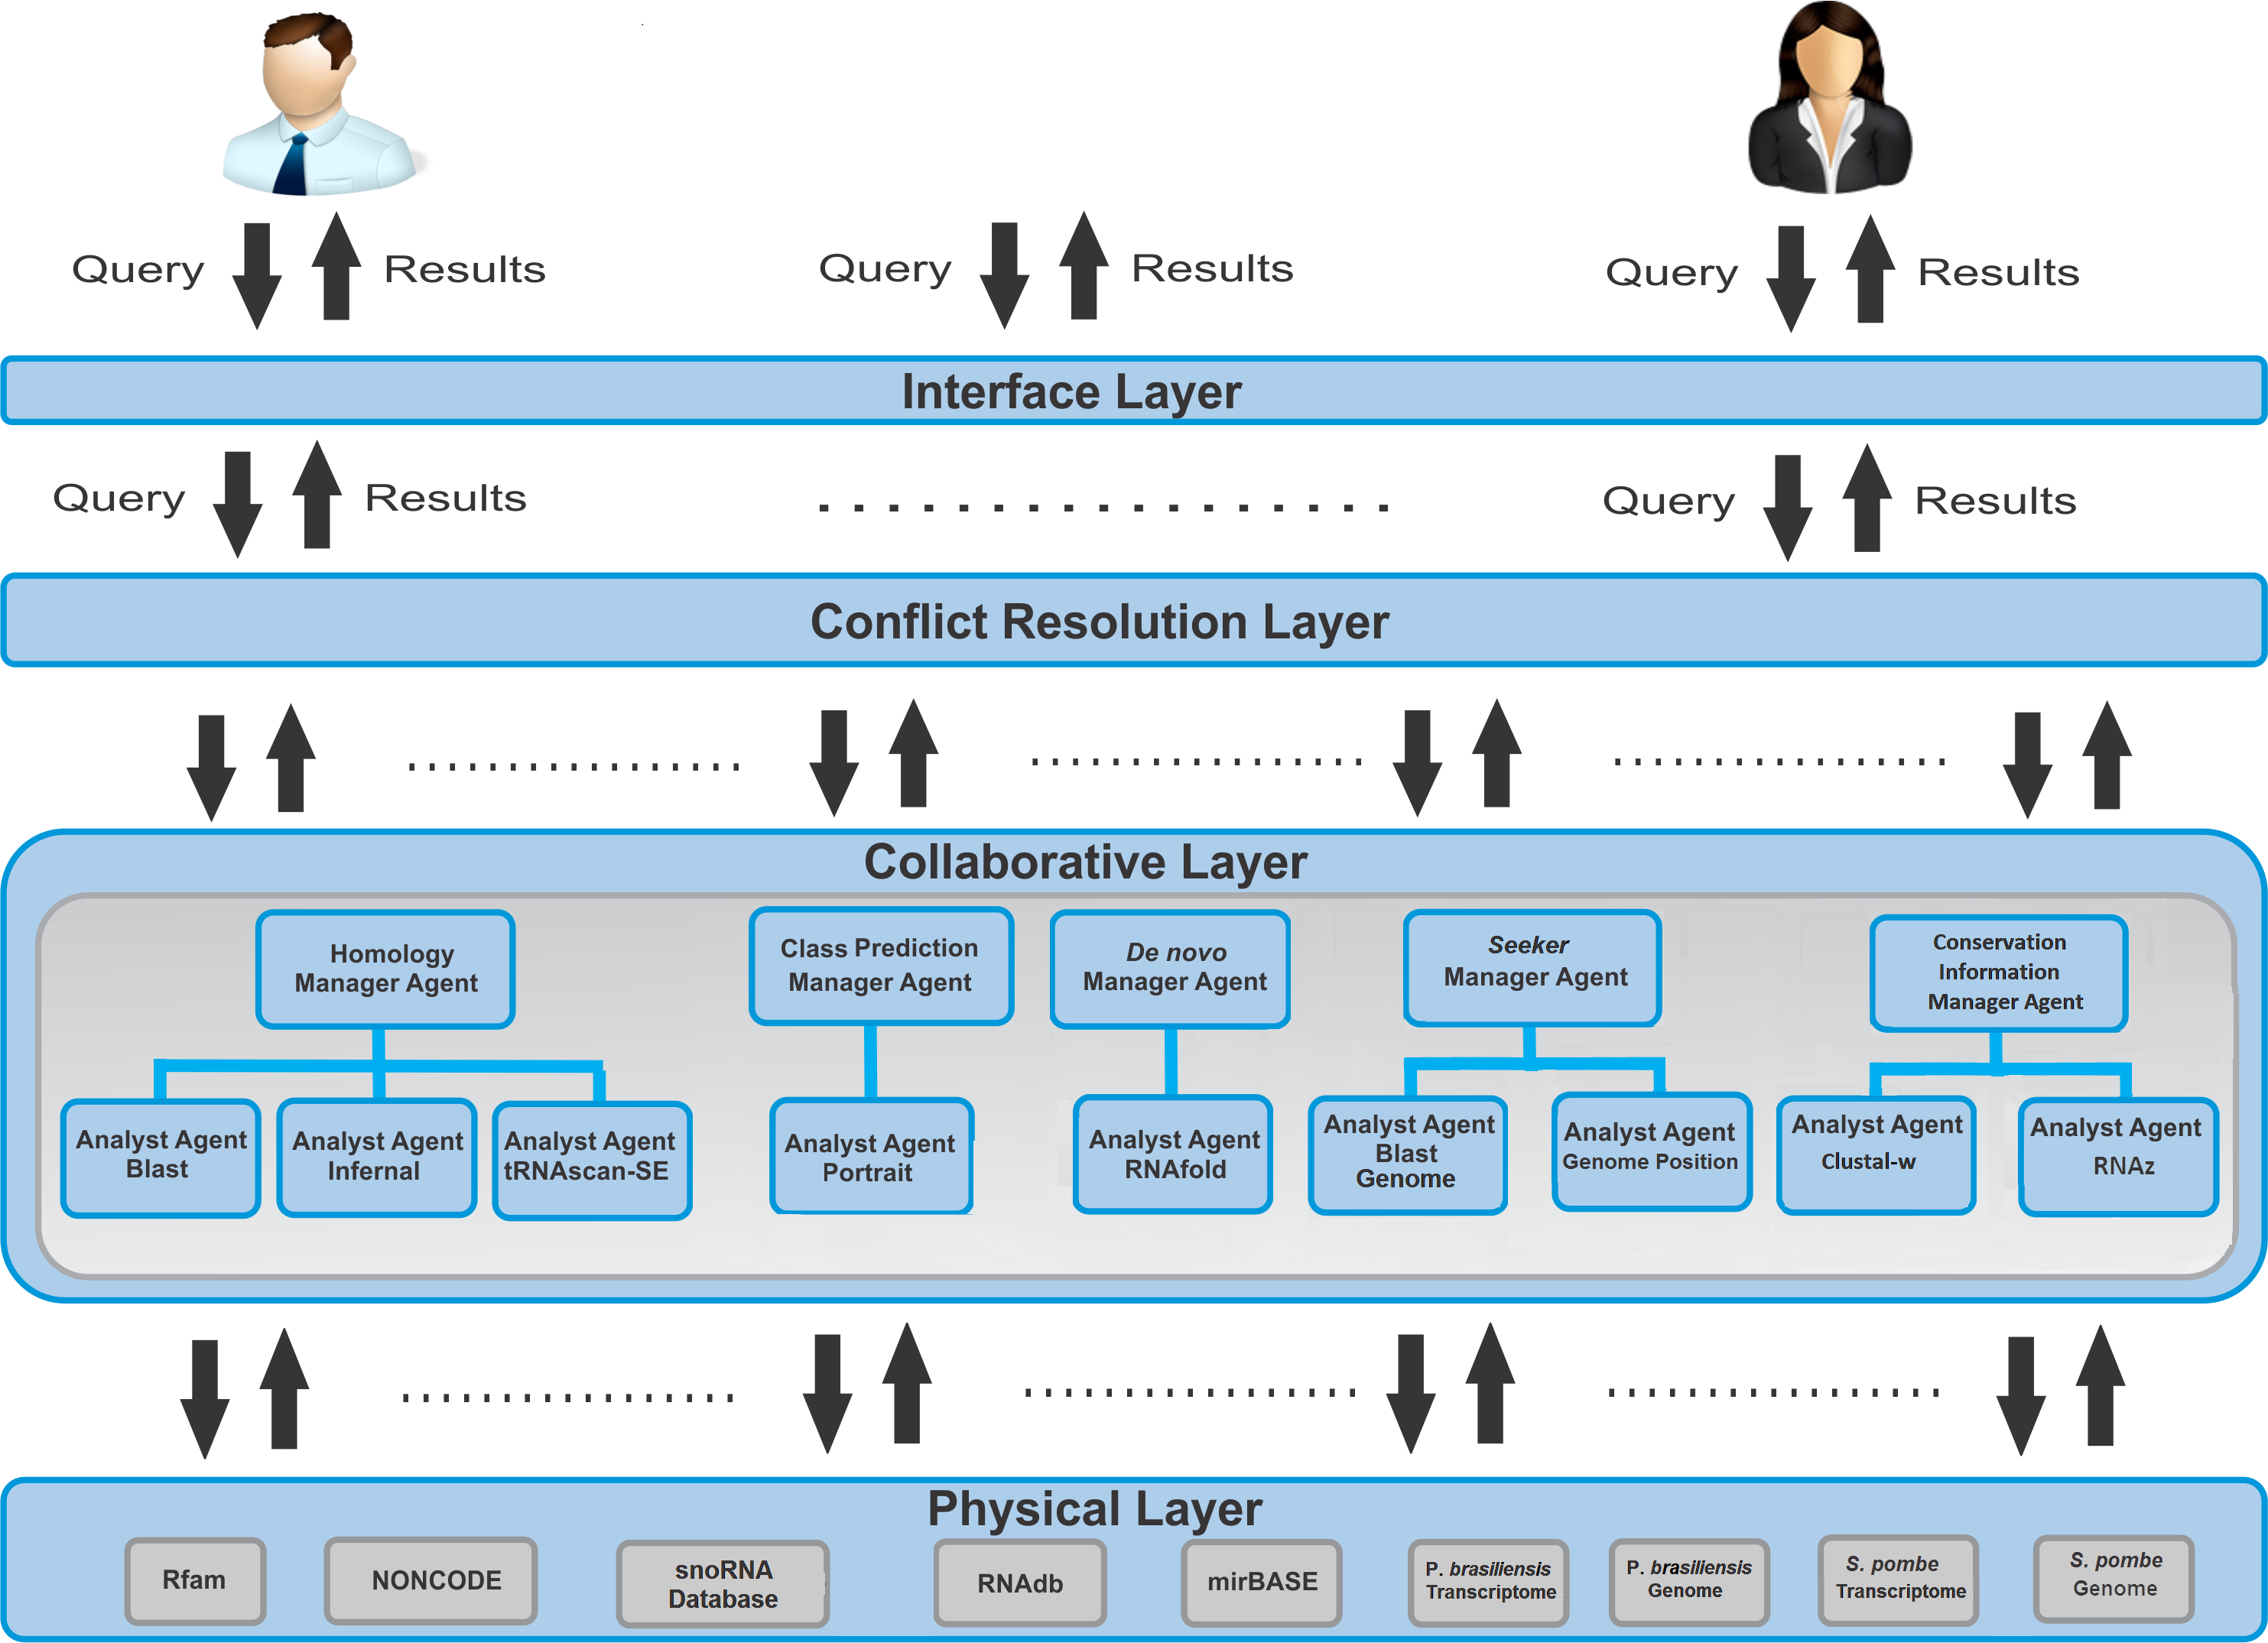
\includegraphics[angle=0,width=1.4\textwidth]{imagens//Arquitetura2sem1.png}
\caption{Arquitetura do ncRNAs-Agents.~\citep{Arruda:2011}. 
\label{fig:441}}
\end{figure}
\end{landscape}


\subsubsection{Descri\c{c}\~ao das Camadas} \label{sec:DescriCamada}

A \textbf{camada de interface} recebe a requisi\c{c}\~ao do usu\'ario composta por um arquivo com sequ\^encias em formato FASTA e indica\c{c}\~ao de ferramentas de anota\c{c}\~ao, e uma retorna os resultados de anota\c{c}\~ao das sequ\^encias de ncRNAs para o usu\'ario. A \textbf{camada de resolu\c{c}\~ao de conflitos} decide qual \'e a melhor recomenda\c{c}\~ao para a anota\c{c}\~ao de cada sequ\^encia recebida da camada de interface, a partir das diversas sugest\~oes recebidas da camada colaborativa, e informa essa decis\~ao para a camada de interface. A \textbf{camada colaborativa} \'e respons\'avel pela execu\c{c}\~ao das diversas ferramentas para identifica\c{c}\~ao e classifica\c{c}\~ao de ncRNAs, enviando os resultados obtidos para a camada de resolu\c{c}\~ao de conflitos. A \textbf{camada f\'isica} \'e formada por banco de dados.

\subsubsection{Descri\c{c}\~ao dos Agentes} \label{sec:DescriAgentes}

Na \textbf{camada colaborativa} existem dois tipos de agentes: \textbf{Agentes Gerentes} e \textbf{Agentes Analistas}. Os \textbf{Agentes Gerentes} realizam um filtro nas sugest\~oes enviadas pelos Agentes Analistas. Temos tr\^es tipos de Agentes Gerentes, conforme as tr\^es abordagens descritas na se\c{c}\~ao \ref{sec:Anotacao}. \textbf{Agente Gerente de Homologia} coordena agentes que trabalham com ferramentas baseadas em homologia. Dois exemplos s\~ao: (i) BLAST~\citep{altschul1990basic:1990}, que considera apenas a estrutura prim\'aria da sequ\^encia e identifica bem os snoRNAs~\citep{durbin1998biological:1998}; e (ii) Infernal~\citep{eddy2003infernal:2003}. O \textbf{Agente Gerente Predi\c{c}\~ao de Classe} coordena os agentes que trabalham com ferramentas baseadas em Aprendizagem de M\'aquina. Um exemplo \'e o SVM-Portrait~\citep{Arrial:2006}. O \textbf{Agente Gerente \textit{De novo}} gerencia agentes que trabalham com ferramentas que não usam organismos de refer\^encia. Um exemplo \'e o RNAz~\citep{washietl2005fast:2005}, do pacote do Vienna, baseados em modelo termodin\^amico. O \textbf{Agente Gerente Alinhamento} coordena agentes que trabalham com ferramentas de alinhamento, resultantes de métodos de comparação de sequência, com o intuito de descobrir motivos comuns ou regi\~oes que permitam verificar se a sequ\^encia \'e de fato um ncRNA.


Os \textbf{Agentes Analistas} s\~ao respons\'aveis por executar ferramentas espec\'ificas para identificar e classificar ncRNAs. Cada Agente Analista, criado por solicita\c{c}\~ao de um Agente Gerente, executa uma an\'alise (\textit{parse}) para extrair informa\c{c}\~oes do arquivo de sa\'ida criado pela ferramenta espec\'ifica controlada por ele. O resultado dessa an\'alise \'e retornado ao Agente Gerente solicitante como recomenda\c{c}\~ao de anota\c{c}\~ao.


\subsection{Detalhes de Implementa\c{c}\~ao} \label{sec:Implemetacao}

Como prova de conceito, foi implementado um prot\'otipo com tr\^es Agentes Gerentes e realizados dois experimentos. 

\subsubsection{Detalhes}


Foi utilizada a plataforma Jade, por diversos motivos: (i) ser distribu\'ido como software sob licen\c{c}a LGPL; (ii) a linguagem de programa\c{c}\~ao suportada ser Java, possibilitando portabilidade; (iii) as especifica\c{c}\~oes de JADE serem compat\'iveis com o padr\~ao FIPA, oferecendo uma biblioteca de classes de protocolos  de intera\c{c}\~ao padronizados e prontas para serem instanciadas; (iv) a disponibiliza\c{c}\~ao da plataforma de agentes, com funcionalidades e ontologia de agentes,  mecanismos transporte e parsing de mensagens; (v) oferece uma comunica\c{c}\~ao eficiente de mensagens entre os agentes com a linguagem ACL~\citep{fipa:2002}, (vi) possui suporte a usu\'arios, tendo uma comunidade grande e ativa de desenvolvedores e vasta documenta\c{c}\~ao dispon\'ivel para consulta.

Foi utilizado o Drools para simula\c{c}\~ao do racioc\'inio por meio de infer\^encias nos agentes, pois permite programar regras de neg\'ocio declarativamente, separar e centralizar as regras de neg\'ocio de um sistema, e gerenciar regras alterando-as dinamicamente.


\subsubsection{Resultados} \label{sec:ResultadosObtidos}

Para a validação do método proposto neste trabalho, foram realizados dois experimentos baseados no Projeto \textit{Paracoccidioides brasilienses} Genoma do (Projeto Genoma Pb) e no Projeto Genoma Guaraná. Ambos os experimentos foram executados tanto para validar o funcionamento do sistema quanto para verificar a acurácia da ferramenta.


A Figura~\ref{sec:Interface} mostra a tela inicial e as ferramentas e bancos de dados já instalados no ncRNA-Agents.

As Figuras \ref{sec:TelaRespostaInfernal} e \ref{sec:TelaFinalExec} mostram \textit{screenshots} de \textit{sniffers} para visualização do comportamento dos agentes do ncRNA-Agents

\begin{landscape}
\begin{figure}[htb!] 
\centering
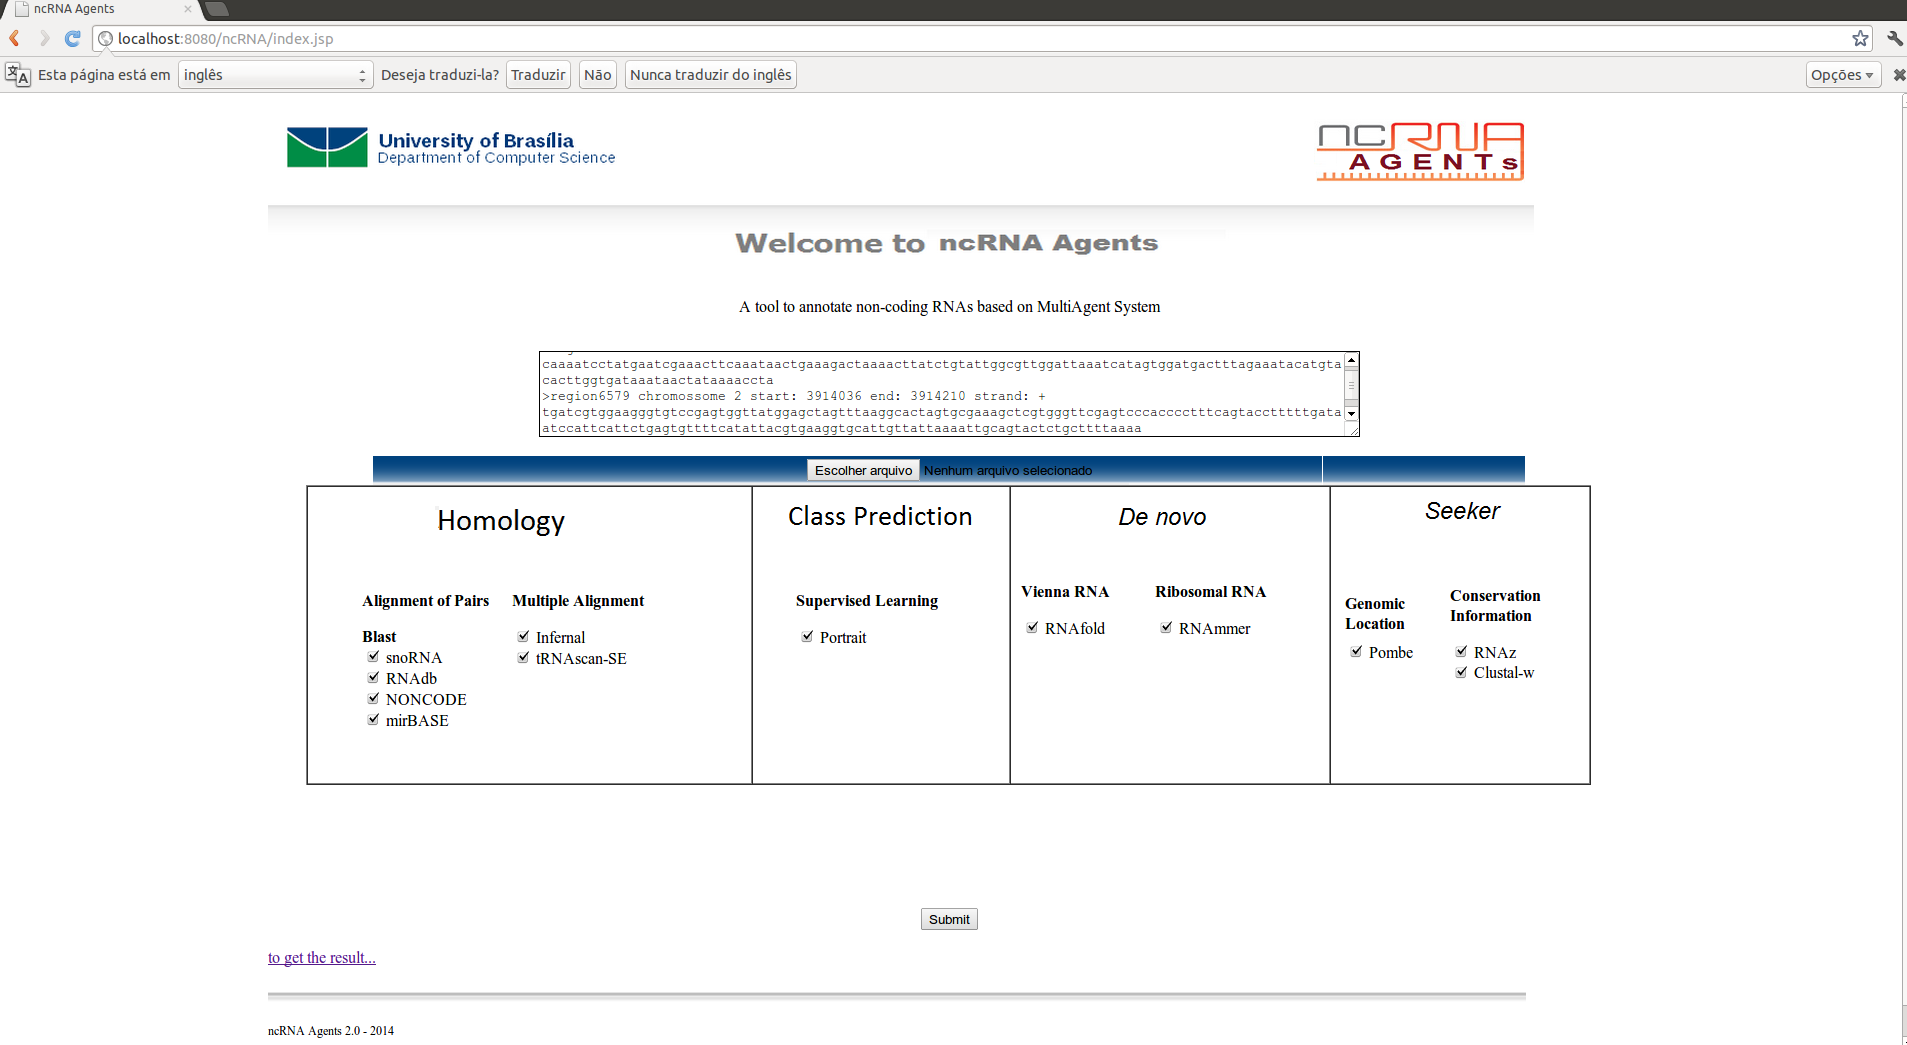
\includegraphics[angle=0,width=1.5\textwidth]{imagens//Interface.png}
\caption{Página do ncRNA-Agents, mostrando as ferramentas e os bancos de dados usados nos experimentos.} \label{sec:Interface}
\end{figure}
\end{landscape}

\begin{landscape}
\begin{figure}[htb!]
\centering
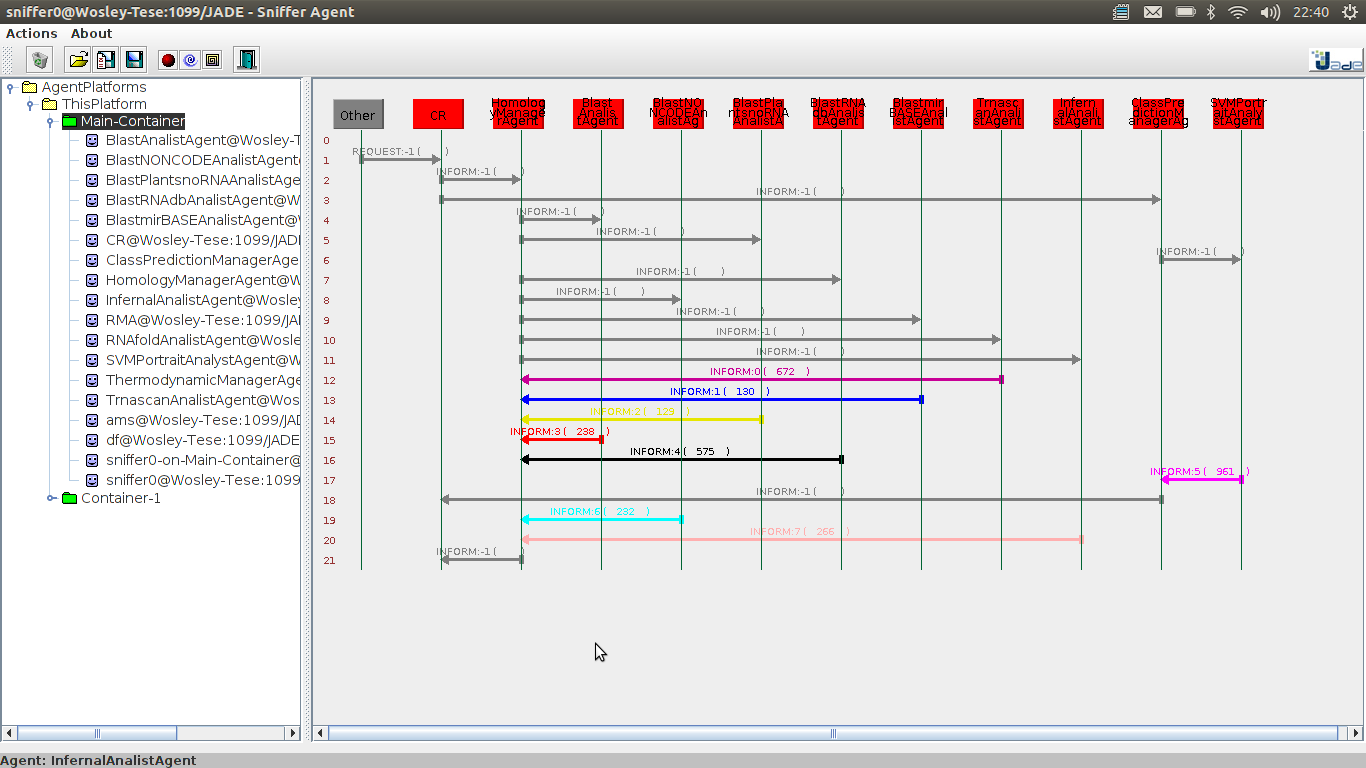
\includegraphics[angle=0,width=1.5\textwidth]{imagens//RespostaInferanal.png}
\caption{\textit{Sniffer} dos agentes do ncRNA-Agents: a camada de resolução de conflitos aguardando a resposta do Agente Gerente Homologia com a ferramenta Infernal.\label{sec:TelaRespostaInfernal}}
\end{figure}
\end{landscape}

\begin{landscape}
\begin{figure}[htb!]
\centering
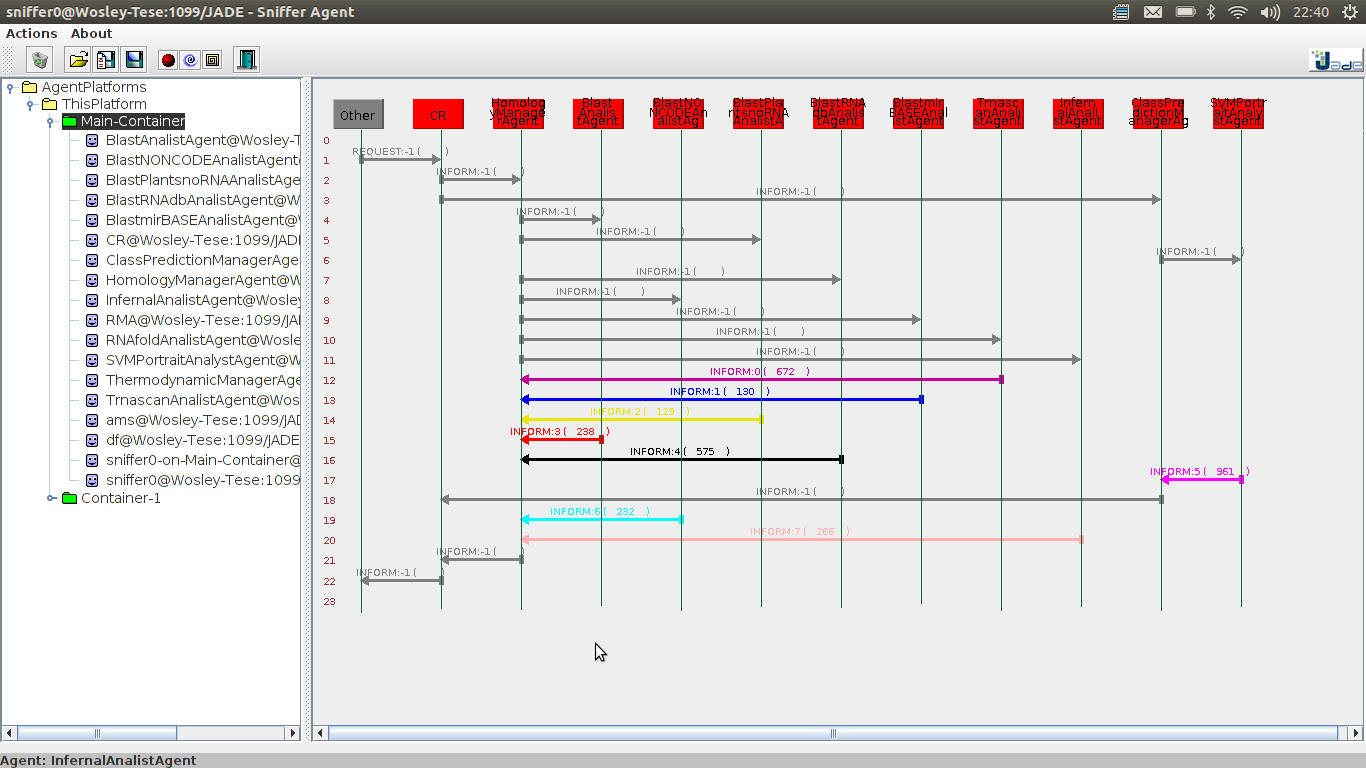
\includegraphics[angle=0,width=1.5\textwidth]{imagens//FinalExe.png}
\caption{\textit{Sniffer} dos agentes do ncRNA-Agents: a camada de resolução de conflitos enviando resposta para a interface do ncRNA-Agents para o usuário.\label{sec:TelaFinalExec}}
\end{figure}
\end{landscape}



\newpage
\subsubsection*{Obtidos} \label{sec:Resulobtidos}

Os estudos de caso foram conduzidos para identificar ncRNAs em dois projetos transcritoma: Projeto Genoma Pb e Projeto Genoma Guaraná. No primeiro, foram utilizados: o BLAST com os bancos de dados snoRNA, RNAdb, NONCODE, mirBASE, Infernal e o banco de Rfam 10.1, trRNAscan-SE e SVM-Portrait. No Projeto Genoma Guaraná, foram usados esses mesmos bancos, além do banco de dados Plant-snoRNA.

Esses estudos foram feitos utilizando 200 sequências de cada projeto, buscando a identificação de ncRNAs, observando-se que ainda não foram identificados ncRNAs nos dois projetos. As Tabelas~\ref{fig:ResulProjPb} e ~\ref{fig:ResulProjGuarana} mostram os resultados obtidos.


\begin{table}[htb!]
\caption{ncRNAs identificados no Projeto Genoma Pb.} \label{fig:ResulProjPb}
\centering
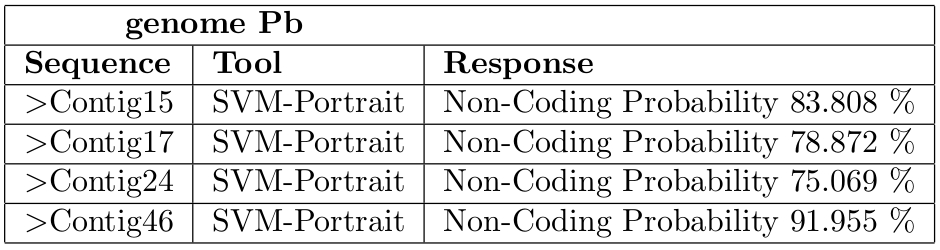
\includegraphics[angle=0,width=0.8\textwidth]{imagens//fig2.JPEG} %\label{fig:AcidosNucleicos}}
\end{table}


\begin{table}[htb!]
\caption{ncRNAs identificados no Projeto Genoma Guaraná.} \label{fig:ResulProjGuarana}
\centering
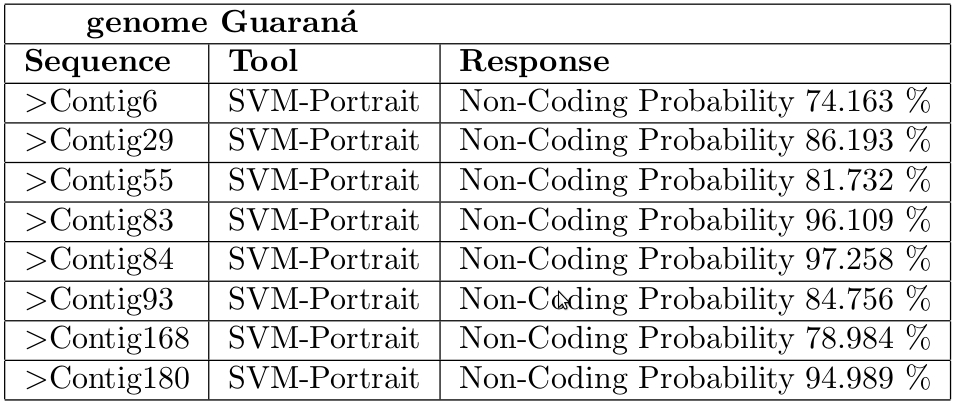
\includegraphics[angle=0,width=0.8\textwidth]{imagens//fig1.JPEG}
\end{table}

\subsubsection*{Esperados} \label{sec:Resulobter}

Os testes nos dois projetos serão estendidos para todas as sequências dos dois Projetos Genoma, Pb (6.022) sequências e Guaraná (8.613).
 % cap 5

  \chapter{Resultados}
\label{sec:Resultados}

Para a validação do método proposto neste trabalho, foram realizados dois experimentos baseados no Projeto \textit{Paracoccidioides brasilienses} Genoma do (Projeto Genoma Pb) e no Projeto Genoma Guaraná. Ambos os experimentos foram executados tanto para validar o funcionamento do sistema quanto para verificar a acurácia da ferramenta.


A Figura \ref{sec:TelaConfig} mostra a tela inicial e as ferramentas e bancos de dados já instalados no ncRNA-Agents.

\begin{figure}[htb!] \label{sec:TelaConfig}
\centering
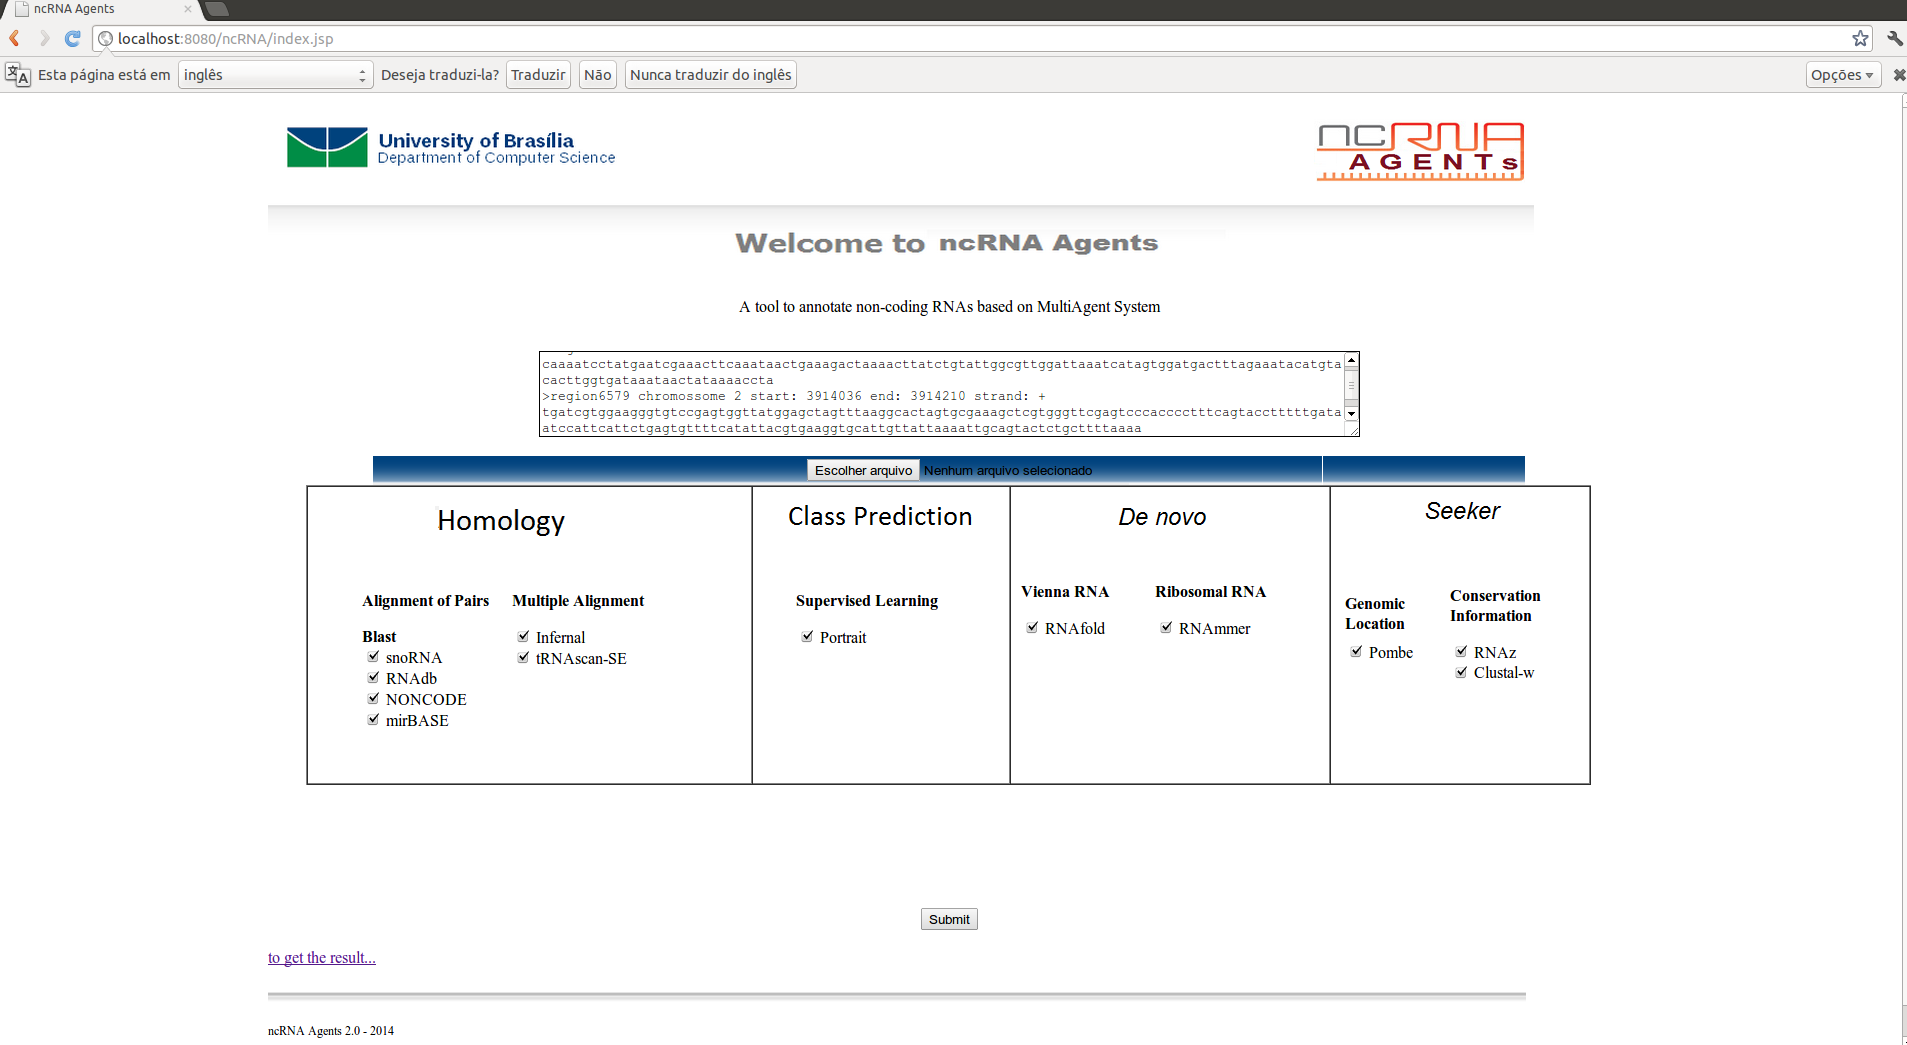
\includegraphics[angle=0,width=1.0\textwidth]{imagens//TelaConfig.png}
\caption{Página do ncRNA-Agents, mostrando as ferramentas e os bancos de dados usados nos experimentos. \label{sec:TelaConfig}}
\end{figure}

A Figura \ref{sec:TelaRespostaInfernal} e \ref{sec:TelaFinalExec} mostram \textit{screenshots} de \textit{sniffers} para visualização do comportamento dos agentes do ncRNA-Agents

\begin{figure}[htb!]
\centering
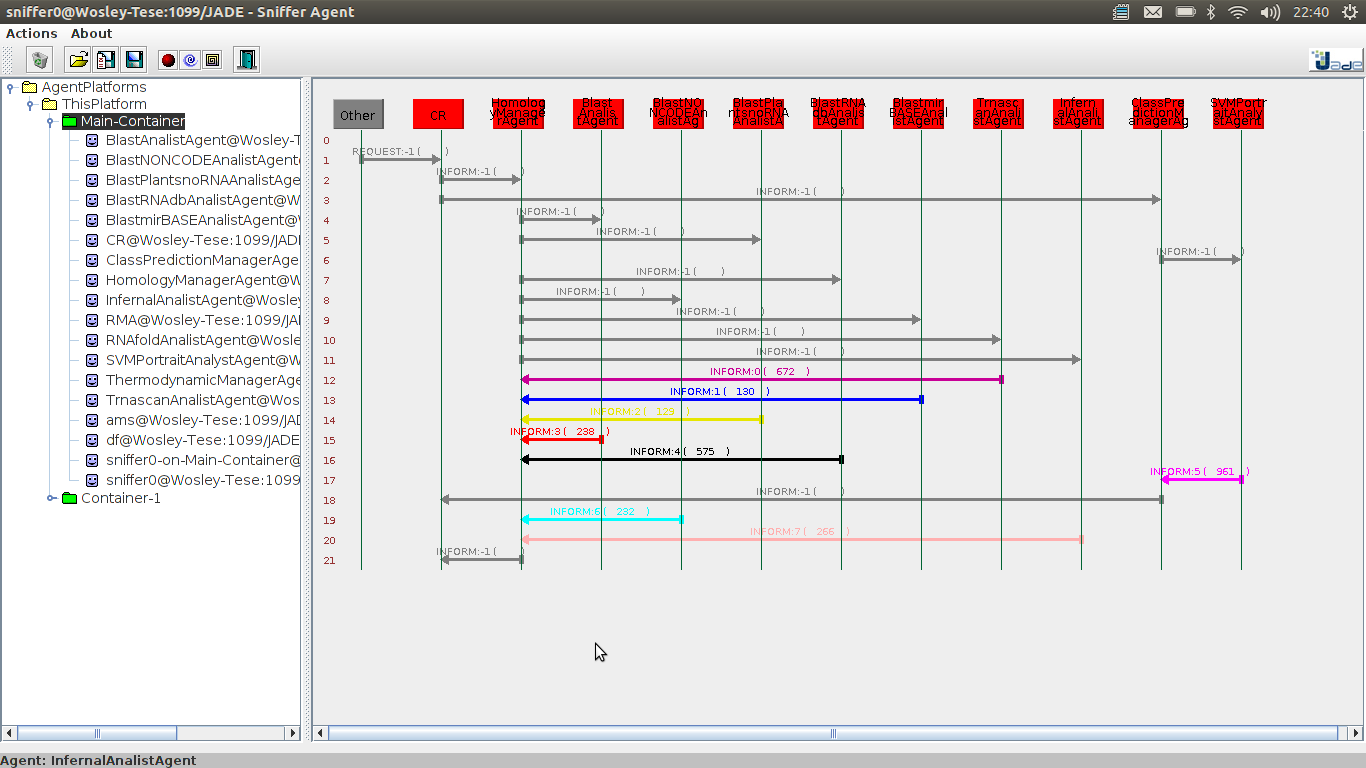
\includegraphics[angle=0,width=0.8\textwidth]{imagens//RespostaInferanal.png}
\caption{\textit{Sniffer} dos agentes do ncRNA-Agents: Aguardando tomada de decisão da camada RC.\label{sec:TelaRespostaInfernal}}
\end{figure}


\begin{figure}[htb!]
\centering
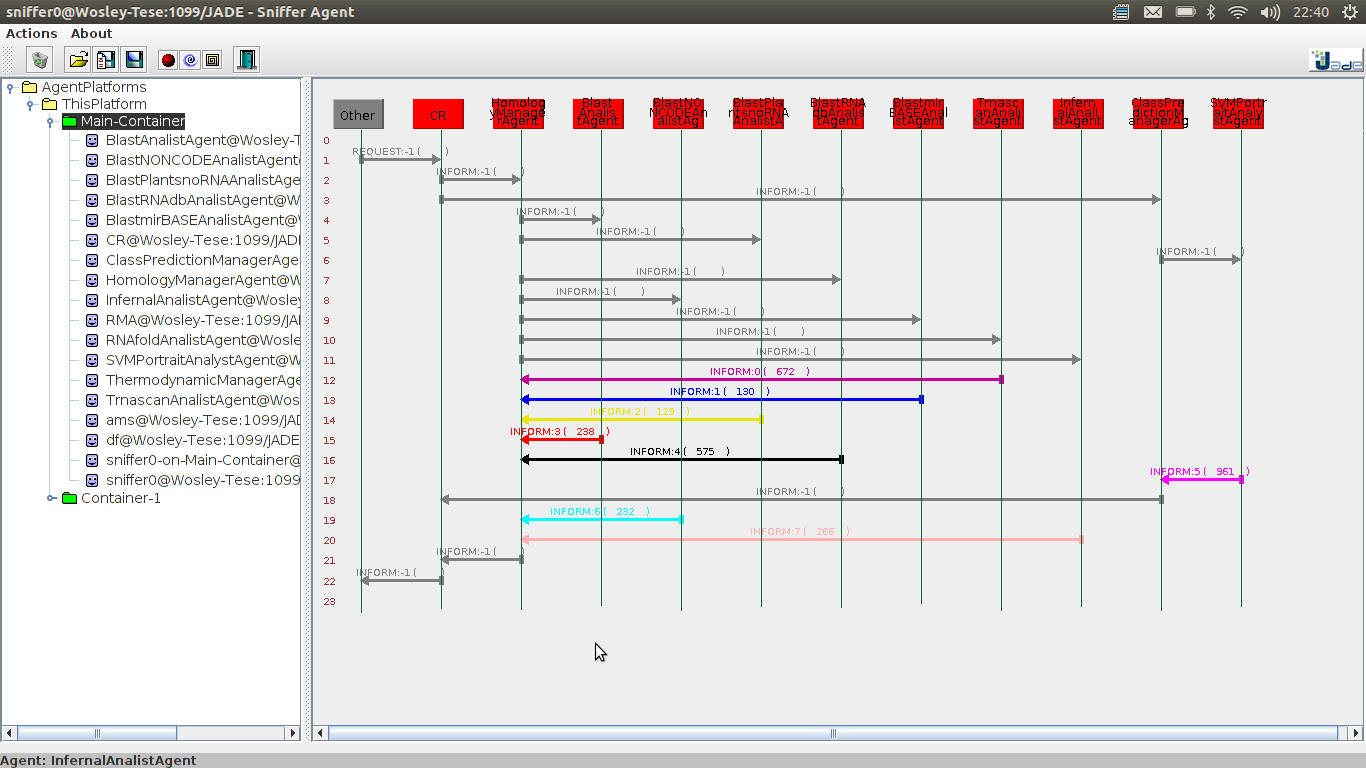
\includegraphics[angle=0,width=0.8\textwidth]{imagens//FinalExe.png}
\caption{\textit{Sniffer} dos agentes do ncRNA-Agents: Enviando resposta para a interface.\label{sec:TelaFinalExec}}
\end{figure}


\newpage
\subsection{Obtidos} \label{sec:Resulobtidos}

Os estudos de caso foram conduzidos para identificar ncRNAs em dois projetos transcritoma: Projeto Genoma Pb e Projeto Genoma Guaraná. No primeiro, foram utilizados: o BLAST com os bancos de dados snoRNA, RNAdb, NONCODE, mirBASE, Infernal e o banco de Rfam 10,1, trRNAscan-SE e SVM-Portrait. No Projeto Genoma Guaraná, foram usados esses mesmos bancos, além do banco de dados Plant-snoRNA.

Esses estudos foram feitos utilizando 200 sequências de cada projeto, buscando a identificação de ncRNAs, observando-se que ainda não foram identificados ncRNAs nos dois projetos. As Tabelas (\ref{fig:ResulProjPb}) e (\ref{fig:ResulProjGuarana}) mostram os resultados obtidos.

\begin{table}[htb!]
\caption{ncRNAs identificados no Projeto Genoma Pb.} \label{fig:ResulProjPb}
\centering
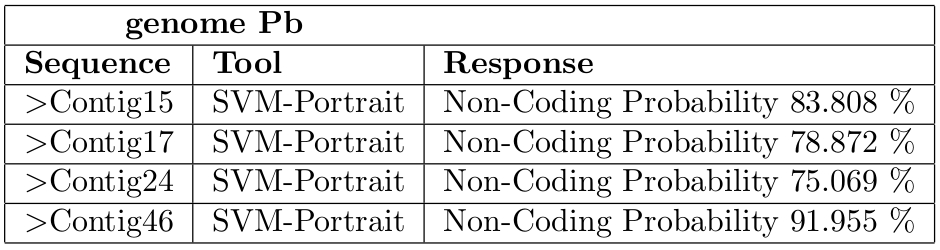
\includegraphics[angle=0,width=0.8\textwidth]{imagens//fig2.JPEG} %\label{fig:AcidosNucleicos}}
\end{table}


\begin{table}[htb!]
\caption{ncRNAs identificados no Projeto Genoma Guaraná.} \label{fig:ResulProjGuarana}
\centering
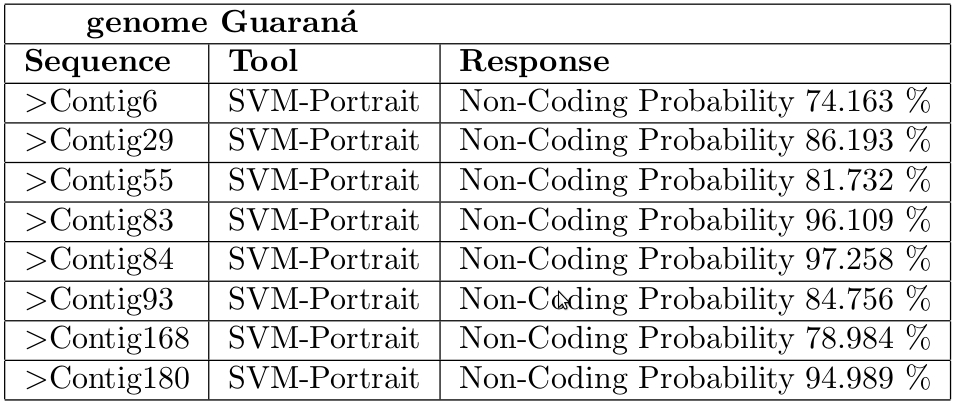
\includegraphics[angle=0,width=0.8\textwidth]{imagens//fig1.JPEG}
\end{table}


\subsubsection{P. brasiliensis} \label{sec:PBrasili}


\subsubsection{P. pombe} \label{sec:SPombe}



%Os testes nos dois projetos serão extendidos para todas as sequências dos dois Projetos Genoma, Pb (6.022) sequências e Guaraná com (8.000).
%
%Será disponibilizado o sistema pela web.
%
%Serão realizados mais experimentos com outros Projetos Genoma.
%
%
%
 % cap 6

  \chapter{Conclusão}
\label{sec:Conclusão}

Neste capítulo descrevemos as atividades do doutorado, as etapas já realizadas e as futuras.


\subsection{Disciplinas} \label{sec:AtividadesRealizadas}



\subsection{Disciplinas} \label{sec:AtividadesRealizadas}

Desde o ingresso no Programa de Pós-graduação em Informática (PPGInf) da
Universidade de Brasília (UnB) em 2010/2 até a data atual, foram cursadas as disciplinas, tendo sido completados 40 créditos (8 com aproveitamento de créditos). 

\subsection{Pesquisa} \label{sec:cronogramaAtividades}

As atividades de pesquisa seguintes já foram concluídas:

\begin{enumerate}
\item Pesquisa: Levantamento do estado da arte sobre anotação de ncRNAs;
\item Estudo de SMA e Motores de Regras de Inferência;
\item Escrita de resumo sobre a ferramenta ncRNA-Agents para o WPOS-2011~\citep{wosley2011:2011};
\item Implementação de protótipos e estudo de caso para verificação da viabilidade do projeto.
\end{enumerate}

A Tabela \ref{tab:cronograma} apresenta o cronograma dos passos descritos na metodologia a ser seguida para a conclusão deste projeto:  

\begin{enumerate}
\item Preparação e Defesa da Qualificação; 
\item Implementação de protótipos;
\item Escrita de Artigos Científicos;
\item Aprimoramento da ferramenta/disponibilização na web;
\item Validação e análise dos resultados;
\item Realização de Doutorado sanduíche na Alemanha: As atividades a serem executadas nesta pesquisa seguem o cronograma apresentado na Tabela \ref{tab:cronograma}.
As atividades referentes ao plano de estudos no exterior serão realizadas no
Grupo de Bioinformática, Departamento de Ciência da Computação da Universidade de Leipzig - Alemanha\footnote{http://www.bioinf.uni-leipzig.de/}, sob supervisão do Professor Peter F. Stadler\footnote{http://www.bioinf.uni-leipzig.de/~studla/}.
\item Escrita da Tese;
\item Defesa.
\end{enumerate}

%\begin{table}[htb!]
%\caption{Cronograma de atividades} \label{tab:cronograma}  
%%Tabela 7: Cronograma de atividades.
%\begin{tabular}{|l|l|l|l|l|l|l|}
%\hline
%\textbf{Descrição das atividades} & \multicolumn{2}{c|}{\textbf{2012}} & \multicolumn{2}{c|}{\textbf{2013}} & \multicolumn{2}{c|}{\textbf{2014}} \\ 
%\cline{2-7}
% & \multicolumn{1}{c|}{\textbf{Ago-Out}} & \textbf{Nov-Dez} & \multicolumn{1}{c|}{\textbf{Jan-Jul}} & \textbf{Ago-Dez} & \multicolumn{1}{c|}{\textbf{Jan-Jun}} & \textbf{Jul} \\ 
%\hline
%\multicolumn{1}{|c|}{\textbf{Preparação e Defesa}} & \multicolumn{1}{c|}{X} & \multicolumn{1}{c|}{} & \multicolumn{1}{c|}{} & \multicolumn{1}{c|}{} & \multicolumn{1}{c|}{} & \multicolumn{1}{c|}{} \\ 
%\multicolumn{1}{|c|}{\textbf{da Qualificação}} & \multicolumn{1}{c|}{} & \multicolumn{1}{c|}{} & \multicolumn{1}{c|}{} & \multicolumn{1}{c|}{} & \multicolumn{1}{c|}{} & \multicolumn{1}{c|}{} \\ 
%\hline
%\multicolumn{1}{|c|}{\textbf{Implementação de}} & \multicolumn{1}{c|}{} & \multicolumn{1}{c|}{X} & \multicolumn{1}{c|}{X} & \multicolumn{1}{c|}{} & \multicolumn{1}{c|}{} & \multicolumn{1}{c|}{} \\ 
%\multicolumn{1}{|c|}{\textbf{protótipos}} & \multicolumn{1}{c|}{} & \multicolumn{1}{c|}{} & \multicolumn{1}{c|}{} & \multicolumn{1}{c|}{} & \multicolumn{1}{c|}{} & \multicolumn{1}{c|}{} \\ 
%\hline
%\multicolumn{1}{|c|}{\textbf{Escrita de Artigos}} & \multicolumn{1}{c|}{} & \multicolumn{1}{c|}{X} & \multicolumn{1}{c|}{X} & \multicolumn{1}{c|}{X} & \multicolumn{1}{c|}{} & \multicolumn{1}{c|}{} \\ 
%\multicolumn{1}{|c|}{\textbf{Científicos}} & \multicolumn{1}{c|}{} & \multicolumn{1}{c|}{} & \multicolumn{1}{c|}{} & \multicolumn{1}{c|}{} & \multicolumn{1}{c|}{} & \multicolumn{1}{c|}{} \\ 
%\hline
%\multicolumn{1}{|c|}{\textbf{Aprimoramento da}} & \multicolumn{1}{c|}{} & \multicolumn{1}{c|}{} & \multicolumn{1}{c|}{X} & \multicolumn{1}{c|}{X} & \multicolumn{1}{c|}{X} & \multicolumn{1}{c|}{} \\ 
%\multicolumn{1}{|c|}{\textbf{ferramenta}} & \multicolumn{1}{c|}{} & \multicolumn{1}{c|}{} & \multicolumn{1}{c|}{} & \multicolumn{1}{c|}{} & \multicolumn{1}{c|}{} & \multicolumn{1}{c|}{} \\ 
%\hline
%\multicolumn{1}{|c|}{\textbf{Validação e análise dos}} & \multicolumn{1}{c|}{} & \multicolumn{1}{c|}{} & \multicolumn{1}{c|}{} & \multicolumn{1}{c|}{X} & \multicolumn{1}{c|}{X} & \multicolumn{1}{c|}{} \\ 
%\multicolumn{1}{|c|}{\textbf{resultados}} & \multicolumn{1}{c|}{} & \multicolumn{1}{c|}{} & \multicolumn{1}{c|}{} & \multicolumn{1}{c|}{} & \multicolumn{1}{c|}{} & \multicolumn{1}{c|}{} \\ 
%\hline
%\multicolumn{1}{|c|}{\textbf{Realização de Doutorado}} & \multicolumn{1}{c|}{} & \multicolumn{1}{c|}{} & \multicolumn{1}{c|}{} & \multicolumn{1}{c|}{X} & \multicolumn{1}{c|}{X} & \multicolumn{1}{c|}{} \\ 
%\multicolumn{1}{|c|}{\textbf{Sanduíche na Alemanha}} & \multicolumn{1}{c|}{} & \multicolumn{1}{c|}{} & \multicolumn{1}{c|}{} & \multicolumn{1}{c|}{} & \multicolumn{1}{c|}{} & \multicolumn{1}{c|}{} \\ 
%\hline
%\multicolumn{1}{|c|}{\textbf{Escrita de Tese}} & \multicolumn{1}{c|}{} & \multicolumn{1}{c|}{} & \multicolumn{1}{c|}{} & \multicolumn{1}{c|}{} & \multicolumn{1}{c|}{X} & \multicolumn{1}{c|}{} \\ 
%\hline
%\multicolumn{1}{|c|}{\textbf{Defesa}} & \multicolumn{1}{c|}{} & \multicolumn{1}{c|}{} & \multicolumn{1}{c|}{} & \multicolumn{1}{c|}{} & \multicolumn{1}{c|}{} & \multicolumn{1}{c|}{X} \\ 
%\hline
%\end{tabular}
%\end{table} % cap 7
 
  \postextual
  \bibliographystyle{plain}
  \bibliography{bibliography}

\end{document}